\PassOptionsToPackage{unicode=true}{hyperref} % options for packages loaded elsewhere
\PassOptionsToPackage{hyphens}{url}
%
\documentclass[]{article}
\usepackage{lmodern}
\usepackage{amssymb,amsmath}
\usepackage{ifxetex,ifluatex}
\usepackage{fixltx2e} % provides \textsubscript
\ifnum 0\ifxetex 1\fi\ifluatex 1\fi=0 % if pdftex
  \usepackage[T1]{fontenc}
  \usepackage[utf8]{inputenc}
  \usepackage{textcomp} % provides euro and other symbols
\else % if luatex or xelatex
  \usepackage{unicode-math}
  \defaultfontfeatures{Ligatures=TeX,Scale=MatchLowercase}
\fi
% use upquote if available, for straight quotes in verbatim environments
\IfFileExists{upquote.sty}{\usepackage{upquote}}{}
% use microtype if available
\IfFileExists{microtype.sty}{%
\usepackage[]{microtype}
\UseMicrotypeSet[protrusion]{basicmath} % disable protrusion for tt fonts
}{}
\IfFileExists{parskip.sty}{%
\usepackage{parskip}
}{% else
\setlength{\parindent}{0pt}
\setlength{\parskip}{6pt plus 2pt minus 1pt}
}
\usepackage{hyperref}
\hypersetup{
            pdftitle={The Woods Hole Assessment Model (WHAM): a general state-space assessment framework that incorporates time- and age-varying processes via random effects and links to environmental covariates},
            pdfauthor={Brian C. Stock1, Timothy J. Miller1},
            pdfborder={0 0 0},
            breaklinks=true}
\urlstyle{same}  % don't use monospace font for urls
\usepackage[margin=1in]{geometry}
\usepackage{graphicx,grffile}
\makeatletter
\def\maxwidth{\ifdim\Gin@nat@width>\linewidth\linewidth\else\Gin@nat@width\fi}
\def\maxheight{\ifdim\Gin@nat@height>\textheight\textheight\else\Gin@nat@height\fi}
\makeatother
% Scale images if necessary, so that they will not overflow the page
% margins by default, and it is still possible to overwrite the defaults
% using explicit options in \includegraphics[width, height, ...]{}
\setkeys{Gin}{width=\maxwidth,height=\maxheight,keepaspectratio}
\setlength{\emergencystretch}{3em}  % prevent overfull lines
\providecommand{\tightlist}{%
  \setlength{\itemsep}{0pt}\setlength{\parskip}{0pt}}
\setcounter{secnumdepth}{5}
% Redefines (sub)paragraphs to behave more like sections
\ifx\paragraph\undefined\else
\let\oldparagraph\paragraph
\renewcommand{\paragraph}[1]{\oldparagraph{#1}\mbox{}}
\fi
\ifx\subparagraph\undefined\else
\let\oldsubparagraph\subparagraph
\renewcommand{\subparagraph}[1]{\oldsubparagraph{#1}\mbox{}}
\fi

% set default figure placement to htbp
\makeatletter
\def\fps@figure{htbp}
\makeatother

\usepackage{url}
\usepackage{setspace}
%\singlespacing
%\onehalfspacing
\doublespacing
\usepackage{lineno}
\linenumbers
\usepackage[belowskip=0pt,aboveskip=0pt]{caption}
\usepackage{relsize}
\usepackage{booktabs}
\usepackage{longtable}
\usepackage{array}
\usepackage{multirow}
\usepackage{wrapfig}
\usepackage{float}
\usepackage{colortbl}
\usepackage{pdflscape}
\usepackage{tabu}
\usepackage{threeparttable}
\usepackage{threeparttablex}
\usepackage[normalem]{ulem}
\usepackage{makecell}
\usepackage{xcolor}

\title{The Woods Hole Assessment Model (WHAM): a general state-space assessment
framework that incorporates time- and age-varying processes via random
effects and links to environmental covariates}
\author{Brian C. Stock\textsuperscript{1}, Timothy J. Miller\textsuperscript{1}}
\date{}

\begin{document}
\maketitle

\(^1\)\href{mailto:brian.stock@noaa.gov}{\nolinkurl{brian.stock@noaa.gov}},
\href{mailto:timothy.j.miller@noaa.gov}{\nolinkurl{timothy.j.miller@noaa.gov}},
Northeast Fisheries Science Center, National Marine Fisheries Service,
166 Water Street, Woods Hole, MA 02543, USA\\

\pagebreak

\hypertarget{abstract}{%
\subsection*{Abstract}\label{abstract}}
\addcontentsline{toc}{subsection}{Abstract}

The rapid changes observed in many marine ecosystems that support
fisheries pose a challenge to stock assessment and management predicated
on time-invariant productivity and considering species in isolation. In
single-species assessments, two main approaches have been used to
account for productivity changes: allowing biological parameters to vary
stochastically over time (empirical), or explicitly linking population
processes such as recruitment (\emph{R}) or natural mortality (\emph{M})
to environmental covariates (mechanistic). Here, we describe the Woods
Hole Assessment Model (WHAM) framework and software package, which
combines these two approaches. WHAM can estimate time- and age-varying
random effects on annual transitions in numbers at age (NAA), \emph{M},
and selectivity, as well as fit environmental time-series with process
and observation errors, missing data, and nonlinear links to \emph{R}
and \emph{M}. WHAM can also be configured as a traditional statistical
catch-at-age (SCAA) model in order to easily bridge from status quo
models and test them against models with state-space and environmental
effects, all within a single framework.

We fit models with and without (independent or autocorrelated) random
effects on NAA, \emph{M}, and selectivity to data from five stocks with
a broad range of life history, fishing pressure, number of ages, and
time-series length. Models that included random effects performed well
across stocks and processes, especially random effects models with a two
dimensional (2D) first-order autoregressive, AR(1), covariance structure
over age and year. We conducted simulation tests and found negligible or
no bias in estimation of important assessment outputs (SSB, \emph{F},
stock status, and catch) when the operating and estimation models
matched. However, bias in SSB and \emph{F} was often non-trivial when
the estimation model was less complex than the operating model,
especially when models without random effects were fit to data simulated
from models with random effects. Bias of the variance and correlation
parameters controlling random effects was also negligible or slightly
negative as expected. Our results suggest that WHAM can be a useful tool
for stock assessment when environmental effects on \emph{R} or \emph{M},
or stochastic variation in NAA transitions, \emph{M}, or selectivity are
of interest. In the U.S. Northeast, where the productivity of several
groundfish stocks has declined, conducting assessments in WHAM with
time-varying processes via random effects or environment-productivity
links may account for these trends and potentially reduce retrospective
bias.

\hypertarget{keywords}{%
\subsubsection*{Keywords}\label{keywords}}
\addcontentsline{toc}{subsubsection}{Keywords}

state-space; stock assessment; random effects; time-varying;
environmental effects; recruitment; natural mortality; Template Model
Builder (TMB)

\pagebreak

\hypertarget{introduction}{%
\section{Introduction}\label{introduction}}

The last two decades have increasingly seen a push for more holistic,
ecosystem-based fisheries management (Larkin 1996; Link 2002). In part,
this is due to the view that considering single species in isolation
produces riskier and less robust outcomes long-term (Patrick and Link
2015). In several high-profile cases, fisheries management has failed to
prevent collapses because they did not reduce fishing pressure in
responses to changes in natural mortality (\(M\)), recruitment, or
migration patterns caused by dynamics external to the stock in question
(Northern cod: Shelton et al. 2006; Rose and Rowe 2015; Gulf of Maine
cod: Pershing et al. 2015; Pacific sardine: Zwolinski and Demer 2012).
This is particularly concerning in the context of climate change and the
wide range of biological processes---often assumed to be constant---in
stock assessments that are likely to be affected (Stock et al. 2011;
Tommasi et al. 2017).

One approach to account for changing productivity is to explicitly link
population processes to environmental covariates in single-species stock
assessments, i.e.~the mechanistic approach \emph{sensu} Punt et al.
(2014). Traditional single-species assessments assume that most
population dynamics processes are constant in time, even though
fisheries scientists have long known about important drivers of
time-varying population processes, e.g.~recruitment, mortality, growth,
and movement (Garstang 1900; Hjort 1914). Effects of the environment or
interactions with other species can be considered contextually, rather
than explicitly as estimated parameters (although temporal variation in
empirical weight and maturity at age can affect reference points).
Despite how counterintuitive this may seem to ecologists and
oceanographers who study such relationships, the evidence for direct
linkages to specific environmental covariates is often weak and can
break down over time (Myers 1998; McClatchie et al. 2010). Additionally,
the primary goal of most assessments is to provide management advice on
near-term sustainable harvest levels---not to explain ecological
relationships. Even if an environmental covariate directly affects fish
productivity, including the effect in an assessment may not improve
management advice if the effect is weak (De Oliveira and Butterworth
2005). Moreover, including environmental effects in an assessment or
management system has been shown to actually provide worse management in
some cases (Walters and Collie 1988; De Oliveira and Butterworth 2005;
Punt et al. 2014). This can be true even in cases of relatively
well-understood mechanistic links between oceanic conditions and fish
populations, as in the case of sea surface temperature and Pacific
sardine (Zwolinski and Demer 2012; Hill et al. 2018). Still,
incorporating mechanistic environment-productivity links in assessments
does have the potential to reduce residual variance, particularly in
periods when few demographic data exist (Shotwell et al. 2014; Miller et
al. 2016).

An alternative approach is to allow biological parameters to vary
stochastically over time, i.e.~the empirical approach \emph{sensu} Punt
et al. (2014). In this case, the variation is caused by a range of
sources that are not explicitly modeled. Statistical catch-at-age (SCAA)
models typically only estimate year-specific fishing mortality (\(F_y\))
and recruitment (\(R_y\)), often as deviations from a mean, \(R_0\),
that may or may not be a function of spawning biomass, e.g.
\(\text{log}R_y = \text{log}R_0 + \epsilon_y\). The main reason that
other parameters are assumed constant is simply that there are not
enough degrees of freedom to estimate many time-varying parameters. A
common solution is to penalize the deviations, e.g.
\(\epsilon_y \sim \mathcal{N}(0,\sigma^2_\epsilon)\), although the
penalty terms, \(\sigma^2_\epsilon\), must be fixed or iteratively tuned
and are therefore somewhat subjective (Methot and Taylor 2011; Methot
and Wetzel 2013; Aeberhard et al. 2018; Xu et al. 2020). State-space
models that treat parameters as unobserved states can, in principle,
avoid such subjectivity by estimating the penalty terms as variance
parameters constraining random effects and maximizing the marginal
likelihood (Thorson 2019). In this way, state-space models can allow
processes to vary in time while simultaneously estimating fewer
parameters.

Although state-space stock assessments have existed for some time
(Mendelssohn 1988; Sullivan 1992; Gudmundsson 1994), the recent
development of Template Model Builder (TMB, Kristensen et al. 2016)
software to perform efficient Laplace approximation has greatly expanded
their use (Nielsen and Berg 2014; Cadigan 2016; Miller et al. 2016). In
addition to the key advantage of objectively estimating variance, or
``data weighting'', parameters, state-space models naturally predict
unobserved states, and therefore handle missing data and short-term
projections in a straightforward way (ICES 2020). In comparisons with
SCAA models, state-space models have been shown to have larger, more
realistic, uncertainty and lower retrospective bias (Miller and Hyun
2018; Stock et al. 2021).

Retrospective bias can occur when changing environmental conditions lead
to changes in productivity that are unaccounted for in stock
assessments, and this is a concern common to several groundfish stocks
on the Northeast U.S. Shelf (Brooks and Legault 2016; Tableau et al.
2018). The Northeast U.S. Shelf ecosystem is rapidly changing, and this
has motivated managers to make the ``continue{[}d{]} development of
stock assessment models that include environmental terms'' a top
priority (Hare et al. 2016). Applications of state-space models with
environmental effects on recruitment, growth, \(M\), and maturity have
proven promising (Miller et al. 2018; Xu et al. 2018; Miller and Hyun
2018; O'Leary et al. 2019). In addition to providing short-term (1-3
years) catch advice with reduced retrospective bias, it is hoped that
environment-linked assessments will help create realistic evaluation of
sustainable stock and harvest levels in the medium-term (3-10 years) for
stocks that have not rebounded in response to dramatic decreases in
\(F\).

To address the needs of fisheries management in a changing climate, we
seek an assessment framework that combines both the empirical and
mechanistic approaches. Namely, it should be able to 1) estimate
time-varying parameters as random effects (i.e.~a state-space model),
and 2) include environmental effects directly on biological parameters.
The framework should also allow for easy testing against status quo SCAA
models to ease gradual adoption through the ``research track'' or
``benchmark'' assessment process (Lynch et al. 2018). The objectives of
this manuscript are to introduce the Woods Hole Assessment Model (WHAM)
framework and demonstrate its ability to:

\begin{enumerate}
\def\labelenumi{\arabic{enumi}.}
\tightlist
\item
  estimate time- and age-varying random effects on annual changes in
  abundance at age, \(M\), and selectivity;
\item
  fit environmental time-series with process and observation error,
  missing data, and a link to a population process;
\item
  project processes treated as random effects in short-term population
  forecasts; and
\item
  simulate new data and random effects to conduct self- and cross-tests
  (\emph{sensu} Deroba et al. 2015) to estimate bias in parameters and
  derived quantities.
\end{enumerate}

Throughout, we describe how the above are implemented using the
open-source WHAM software package (Miller and Stock 2020).

\hypertarget{methods}{%
\section{Methods}\label{methods}}

\hypertarget{model-description}{%
\subsection{Model description}\label{model-description}}

WHAM is a generalization and extension of Miller et al. (2016) in TMB.
It is in many respects similar to the Age-Structured Assessment Program
(ASAP, Legault and Restrepo 1998; Miller and Legault 2015) and can be
configured to fit statistical catch-at-age models nearly identically.
There is functionality built into WHAM to migrate ASAP input files to R
inputs needed for WHAM, and WHAM uses many of the same types of data
inputs, such as empirical weight-at-age, so that existing assessments in
the U.S. Northeast can be easily replicated and tested against models
with state-space and environmental effects in a single framework.

\hypertarget{processes-with-random-effects}{%
\subsubsection{Processes with random
effects}\label{processes-with-random-effects}}

WHAM primarily diverges from ASAP through the implementation of random
effects on three processes: inter-annual transitions in numbers at age
(\emph{NAA}), natural mortality (\emph{M}), and selectivity (\emph{s}),
as well as allowing effects of environmental covariates (\emph{Ecov}) on
recruitment and natural mortality (but see ASAP4; Miller and Legault
2015). The environmental covariates and their observations are part of
the state-space framework with true, unobserved values treated as random
effects and observation on them having error. Other than environmental
covariates, the processes are assumed to have a two dimensional (2D)
first-order autoregressive, AR(1), covariance structure over age and
year, although correlation in either or both dimensions can be turned
off. The 2D AR(1) structure has been widely used to model deviations by
age and year in the parameters \(F_{a,y}\) (Nielsen and Berg 2014; Kumar
et al. 2020; Perreault et al. 2020), \(M_{a,y}\) (Cadigan 2016; Stock et
al. 2021), \(s_{a,y}\) (Xu et al. 2019), and \(N_{a,y}\) (Stock et al.
2021), as well as in the catch (\(C_{a,y}\)) and survey index
(\(I_{a,y}\)) observations (Berg and Nielsen 2016). Although other
covariance structures are plausible (e.g.~compound symmetry,
unconstrained, or order-\emph{k} autoregressive; Nielsen and Berg 2014;
Berg and Nielsen 2016), the 2D AR(1) structure is a simple option which
requires few parameters and allows for smooth deviations in time and by
age; values for nearby years and ages are more correlated than distant
ones. This is often a reasonable null hypothesis for biological or
fishery processes, but there are also clear examples where change occurs
abruptly, e.g.~a disease outbreak increases \emph{M} or changes in gear
or area regulations affect selectivity (ICES 2017a).

\hypertarget{numbers-at-age-naa}{%
\paragraph{\texorpdfstring{Numbers at age
(\emph{NAA})}{Numbers at age (NAA)}}\label{numbers-at-age-naa}}

The stock equations in WHAM that describe the transitions between
numbers at age are identical to Miller et al. (2016) and Nielsen and
Berg (2014):

\begin{equation}
\label{eq:NAA}
  \text{log}N_{a,y}=\left\{
    \begin{array}{@{}lll@{}}
      \text{log} \left( f(SSB_{y-1}) \right) + \varepsilon_{1,y}, & \text{if}\ a = 1 \\
      \text{log} \left( N_{a-1,y-1} \right) - Z_{a-1,y-1} + \varepsilon_{a,y}, & \text{if}\ 1 < a < A \\
      \text{log} \left( N_{A-1,y-1} e^{-Z_{A-1,y-1}} + N_{A,y-1} e^{-Z_{A,y-1}} \right) + \varepsilon_{A,y}, & \text{if}\ a = A
    \end{array}\right.
\end{equation}

where \(N_{a,y}\) are the numbers at age \emph{a} in year \emph{y},
\emph{Z} is the total mortality rate (\(F + M\)), \(f\) is the
stock-recruit function (for options see
\protect\hyperlink{appendix-a}{Appendix A}), and \emph{A} represents the
plus-group. The \(\varepsilon_{a,y}\) deviations are akin to survival,
which is clearly related to \(M_{a,y}\), but they can also be caused by
mis-specification of selectivity of the fishery or indices, movement
into or out of the population, or misreported catch (Schnute and
Richards 1995; Gudmundsson and Gunnlaugsson 2012; Perretti et al. 2020;
Stock et al. 2021). In this analysis we consider the SCAA model,
``Base'', and then examine four possible models that treat the
\(\varepsilon_{a,y}\) deviations as random effects.

Base is a SCAA model, which estimates recruitment deviations,
\(\varepsilon_{1,y}\), in each year \(y > 1\) as unconstrained fixed
effect parameters. The \emph{NAA} deviations for ages \(a > 1\) are
fixed at zero so that transitions are deterministic.

NAA-1 is most similar to Base, where only recruitment deviations,
\(\varepsilon_{1,y}\), are estimated. However, in NAA-1 the recruitment
deviations are assumed to be independent and identically distributed
(IID) random effects,

\[\varepsilon_{1,y} \sim \mathcal{N}\left( - \frac{\sigma^2_R}{2}, \sigma^2_R \right),\]
with variance \(\sigma^2_R\) as an estimated parameter. The
\(- \frac{\sigma^2_R}{2}\) bias correction term is included by default
so that the expected recruitment, \(E(N_{1,y} = R_y)\) equals the
expected \(R_y\) from the stock-recruit function (Methot and Taylor
2011; Thorson 2019). This bias correction adjustment can also be turned
off.

NAA-2 is the same as NAA-1, except that the recruitment deviations are
stationary AR(1) with autocorrelation parameter \(-1<\rho_{year}<1\):

\[\varepsilon_{1,y+1} \sim \mathcal{N}\left(\rho_{year} \varepsilon_{1,y} - \frac{\sigma^2_R}{2 (1-\rho^2_{year})}, \sigma^2_R \right)\]

NAA-3 is the ``full state-space'' model from Nielsen and Berg (2014) and
Miller et al. (2016), where all numbers at age are independent random
effects and:

\begin{equation}
  \varepsilon_{a,y} \sim \left\{
    \begin{array}{@{}ll@{}}
      \mathcal{N} \left( - \frac{\sigma^2_R}{2}, \sigma^2_R \right), & \text{if}\ a = 1 \\
      \mathcal{N} \left( - \frac{\sigma^2_a}{2}, \sigma^2_a \right), & \text{if}\ a > 1
    \end{array}\right.
\end{equation}

where \(\sigma^2_a\) for all ages \(a > 1\) are assumed to be the same
but different from age \(a = 1\), i.e.~recruitment. This assumption is
sensible because variability of deviations between expected and realized
recruitment are typically larger than deviations from expected abundance
at older ages.

NAA-4 treats the numbers at all ages as random effects, as in NAA-3, but
the \emph{NAA} deviations, \(\varepsilon_{a,y}\), have a 2D stationary
AR(1) structure as in Stock et al. (2021):

\[\mathbf{E} \sim \mathcal{MVN} \left( 0, \Sigma \right)\]

where
\(\mathbf{E} = (\varepsilon_{1,1}, \ldots, \varepsilon_{1,Y-1}, \varepsilon_{2,1}, \ldots, \varepsilon_{2,Y-1}, \ldots, \varepsilon_{A,1}, \ldots, \varepsilon_{A,Y-1})'\)
is a vector of all \emph{NAA} deviations, \emph{Y} is the total number
of observation and prediction years, and \(\boldsymbol{\Sigma}\) is the
covariance matrix of \(\mathbf{E}\) defined by:

\[ \text{Cov} \left( \varepsilon_{a,y}, \varepsilon_{\tilde{a},\tilde{y}} \right) = \frac{\sigma_a \sigma_{\tilde{a}} \rho^{|a-\tilde{a}|}_{age} \rho^{|y-\tilde{y}|}_{year}}{\left(1-\rho^2_{age}\right) \left(1-\rho^2_{year}\right)}\]
and \(-1<\rho_{age}<1\) and \(-1<\rho_{year}<1\) are the AR(1)
coefficients in age and year, respectively. As in NAA-3, \(\sigma^2_a\)
for all ages \(a > 1\) are assumed to be the same but different from age
\(a = 1\), \(\sigma^2_R\). The bias correction term for age \(a > 1\) in
NAA-4 is \(- \frac{\sigma^2_a}{2 (1-\rho^2_{year})(1-\rho^2_{age})}\).

\hypertarget{natural-mortality-m}{%
\paragraph{\texorpdfstring{Natural mortality
(\emph{M})}{Natural mortality (M)}}\label{natural-mortality-m}}

For natural mortality, there are mean parameters for each age,
\(\mu_{M_a}\), each of which may be estimated freely or fixed at the
initial values. The \(\mu_{M_a}\) may also be estimated in sets of ages,
e.g.~estimate one mean \emph{M} shared across ages 3-5,
\(\mu_{M_3} = \mu_{M_4} = \mu_{M_5}\). There is also an option for
\emph{M} to be specified as a function of weight-at-age,
\(M_{a,y} = \mu_M \text{W}^b_{a,y}\), as in Lorenzen (1996) and Miller
and Hyun (2018). Regardless of whether \(\mu_{M_a}\) are fixed or
estimated, WHAM can also be configured to estimate deviations in
\emph{M}, \(\delta_{a,y}\), as random effects analogous to the
\emph{NAA} deviations (Cadigan 2016; Stock et al. 2021):

\begin{equation}
  \begin{array}{cc}
    \text{log}\left( M_{a,y} \right) = \mu_{M_a} + \delta_{a,y} \\
    \text{Cov} \left( \delta_{a,y}, \delta_{\tilde{a},\tilde{y}} \right) = \frac{\sigma^2_M \varphi^{|a-\tilde{a}|}_{age} \varphi^{|y-\tilde{y}|}_{year}}{\left(1-\varphi^2_{age}\right) \left(1-\varphi^2_{year}\right)}
  \end{array}
\end{equation}

where \(\sigma^2_M\), \(\varphi_{age}\), and \(\varphi_{year}\) are the
AR(1) variance and correlation coefficients in age and year,
respectively.

In this analysis, we demonstrate three alternative \emph{M} random
effects models. For simplicity, all models treat \(\mu_{M_a}\) as known,
as in most of the original assessments. M-1 is identical to the NAA-1
model, with no random effects on \emph{M} (\(\delta_{a,y} = 0\) and not
estimated). M-2 allows IID \emph{M} deviations, estimating
\(\sigma^2_M\) but fixing \(\varphi_{age} = \varphi_{year} = 0\). M-3
estimates the full 2D AR(1) structure for \emph{M} deviations.

\hypertarget{selectivity-sel}{%
\paragraph{\texorpdfstring{Selectivity
(\emph{Sel})}{Selectivity (Sel)}}\label{selectivity-sel}}

As in ASAP and many other SCAA assessment frameworks, WHAM assumes
separability in the fishing mortality rate by age and year, e.g.
\(F_{a,y} = F_y s_a\), where \(F_y\) is the ``fully selected'' fishing
mortality rate in year \emph{y} and \(s_a\) is the selectivity at age
\emph{a}. We note that this differs from the approach in SAM (Nielsen
and Berg 2014), where the \(F_{a,y}\) are estimated directly as
multivariate random effects without the separability assumption. Three
parametric forms are available (logistic, double-logistic, and
decreasing-logistic), as well as a non-parametric option to estimate
each \(s_a\) individually (``age-specific''). WHAM estimates selectivity
parameters on the logit scale to avoid boundary problems during
estimation. To allow for abrupt temporal changes in selectivity as in
ASAP, WHAM can estimate selectivity in user-specified time blocks. WHAM
can also estimate smooth changes in selectivity using autoregressive
random effects as described below.

WHAM estimates annual full \(F_y\) and mean selectivity parameters as
fixed effects. Deviations in selectivity parameters can be estimated as
random effects, \(\zeta_{p,y}\), with autocorrelation by parameter
(\emph{p}), year (\emph{y}), both, or neither. This is done similarly to
Xu et al. (2019), except that the deviations are placed on the
parameters instead of the mean \(s_{a,y}\) in order to guarantee that
\(0 < s_{a,y} < 1\). For example, logistic selectivity with two
parameters \(a_{50}\) and \(k\) is estimated as:

\begin{equation}
  \begin{array}{cccc}
    s_{a,y} = \frac{1}{1 + e^{-(a - a_{{50}_y}) / k_y}} \\
    a_{{50}_y} = l_{a_{50}} + \frac{u_{a_{50}} - l_{a_{50}}}{1 + e^{-(\nu_1 + \zeta_{1,y})}} \\
    k_y = l_k + \frac{u_k - l_k}{1 + e^{-(\nu_2 + \zeta_{2,y})}} \\
    \text{Cov} \left( \zeta_{1,y}, \zeta_{2,\tilde{y}} \right) = \frac{\sigma^2_s \phi_{par} \phi^{|y-\tilde{y}|}_{year}}{\left(1-\phi^2_{par}\right) \left(1-\phi^2_{year}\right)}
  \end{array}
\end{equation}

where \(\nu_1\) is the logit-scale mean \(a_{50}\) parameter with lower
and upper bounds \(l_{a_{50}}\) and \(u_{a_{50}}\), \(\nu_2\) is the
logit-scale mean \(k\) parameter with lower and upper bounds \(l_k\) and
\(u_k\), \(\sigma^2_s\) is the AR(1) variance, and \(\phi_{par}\), and
\(\phi_{year}\) are the AR(1) correlation coefficients by parameter and
year.

Below, we demonstrate three models with random effect deviations on
logistic selectivity, akin to those for \emph{M}. Sel-1 treats all
numbers at age as independent random effects (i.e.~NAA-3) but with no
random effects on \emph{s} (\(\zeta_{p,y} = 0\) and not estimated).
Sel-2 allows IID \emph{s} random effects, estimating \(\sigma^2_s\) but
fixing \(\phi_{par} = \phi_{year} = 0\). Sel-3 estimates the full 2D
AR(1) structure for \emph{s} random effects.

\hypertarget{environmental-covariates-ecov}{%
\paragraph{\texorpdfstring{Environmental covariates
(\emph{Ecov})}{Environmental covariates (Ecov)}}\label{environmental-covariates-ecov}}

WHAM models environmental covariate data using state-space models with
process and observation components. The true, unobserved values (or
``latent states'', \(X_y\)) are then linked to the population dynamics
equations with user-specified lag, \(\psi\). For example, recruitment in
year \emph{y} may be influenced by \(X\) in the previous year,
\(X_{y-1}\) (\(\psi = 1\)), while natural mortality in year \emph{y} may
be influenced by \(X_y\) (\(\psi = 0\)). Multiple environmental
covariates may be included, but currently only as independent processes.
The environmental and population model years do not need to match, and
missing years are allowed. In particular, including environmental data
in the projection period can be useful.

\hypertarget{ecov-process-model}{%
\subparagraph{\texorpdfstring{\emph{Ecov} process
model}{Ecov process model}}\label{ecov-process-model}}

There are currently two options in WHAM for the \emph{Ecov} process
model: a normal random walk and AR(1). We model the random walk as in
Miller et al. (2016):

\[X_{y+1} | X_y \sim \mathcal{N}\left( X_y, \sigma^2_X\right)\]

where \(\sigma^2_X\) is the process variance and \(X_1\) is estimated as
a fixed effect parameter. One disadvantage of the random walk is that it
is nonstationary. In short-term projections, \(\hat{X}_y\) will be equal
to the last estimate with an observation and the uncertainty of
\(\hat{X}_y\) will increase over time. If \(\hat{X}_y\) influences the
dynamices of the population and reference points, this leads to
increasing uncertainty in projections of the stock and status over time
as well (Miller et al. 2016). For this reason, we generally prefer to
model \(X_y\) as a stationary AR(1) process as in Miller et al. (2018):

\begin{equation}
  \begin{array}{cc}
    X_1 \sim \mathcal{N} \left( \mu_X, \frac{\sigma^2_X}{1-\phi^2_X} \right) \\
    X_y \sim \mathcal{N} \left( \mu_X(1-\phi_X) + \phi_X X_{y-1}, \sigma^2_X \right)
  \end{array}
\end{equation}

where \(\mu_X\), \(\sigma^2_X\), and \(|\phi_X| < 1\) are the marginal
mean, conditional variance, and autocorrelation parameters. In addition
to stationarity, another important difference between the random walk
and AR(1) in short-term population projections is that the AR(1) will
gradually revert to the mean over time, unless environmental covariate
observations are included in the projection period.

\hypertarget{ecov-observation-model}{%
\subparagraph{\texorpdfstring{\emph{Ecov} observation
model}{Ecov observation model}}\label{ecov-observation-model}}

The environmental covariate observations, \(x_y\), are assumed to be
normally distributed with mean \(X_y\) and variance \(\sigma^2_{x_y}\):

\[x_y | X_y \sim \mathcal{N}\left( X_y, \sigma^2_{x_y} \right)\]

The observation variance in each year, \(\sigma^2_{x_y}\), can be
treated as known with year-specific values (as in Miller et al. 2016) or
one overall value shared among years. They can also be estimated as
parameters, likewise either as yearly values or one overall value. If
yearly \(\sigma^2_{x_y}\) estimates are desired, WHAM estimates the
hyperparameters \(\mu_{\sigma_x}\) and \(\sigma_{\sigma_x}\) as fixed
effects and treats the \(\sigma^2_{x_y}\) as random effects:

\[\sigma^2_{x_y} \sim \mathcal{N} \left( \mu_{\sigma_x}, \sigma^2_{\sigma_x} \right)\]

\hypertarget{link-to-population}{%
\subparagraph{Link to population}\label{link-to-population}}

WHAM currently provides options to link the modeled environmental
covariate, \(X_y\), to the population dynamics via recruitment or
natural mortality. It is also sometimes useful to fit the \emph{Ecov}
model without a link to the population dynamics so that models with and
without environmental effects have the same data in the likelihood and
can be compared via AIC.

In the case of recruitment, the options follow the framework laid out by
Fry (1971) and Iles and Beverton (1998): ``controlling''
(density-independent mortality), ``limiting'' (carrying capacity effect,
e.g. \(X_y\) determines the amount of suitable habitat), ``lethal''
(threshold effect, i.e. \(R_y\) goes to 0 at some \(X_y\) value),
``masking'' (\(X_y\) decreases \(\text{d}R/\text{d}SSB\), as expected if
\(X_y\) affects metabolism or growth), and ``directive''
(e.g.~behavioral). Of these, WHAM currently allows controlling,
limiting, or masking effects in the Beverton-Holt stock-recruit
function, and controlling or masking effects in the Ricker function (see
\protect\hyperlink{appendix-a}{Appendix A} for all equations).

For natural mortality, environmental effects are placed on \(\mu_M\),
shared across ages by default. This is the simplest assumption; linking
an environmental covariate to \(M\) affects \(M\) at all ages
identically, i.e. \(M_{a,y} = \mu_{M_a} e^{\beta X_{y-\psi}}\). This
could be modified in the future to estimate different effects on
different ages by changing \(\beta\) from a scalar to a vector of
\(\beta_a\).

Regardless of where the environment-population link is, the effect can
be either linear or polynomial. Nonlinear effects of environmental
covariates are common in ecology, and quadratic effects are to be
expected in cases where intermediate values are optimal (Brett 1971;
Agostini et al. 2008). WHAM includes a function to calculate orthogonal
polynomials in TMB, akin to the \texttt{poly()} function in \texttt{R}.
Orthogonal polynomials remove correlation between covariates, e.g. \(X\)
and \(X^2\), which improves estimability and allows for straightforward
evaluation of the significance of adding \(X^2\) to a model that
includes \(X\).

In this analysis, we compare five models with limiting effects on
Beverton-Holt recruitment:

\begin{equation}
\label{eq:predR}
  \begin{array}{ccc}
    \hat{R}_{y+1} = \frac{\alpha \text{SSB}_{y}}{1 + e^{\beta_0 + \beta_1 X_{y} + \beta_2 X^2_{y}} \text{SSB}_y}
  \end{array}
\end{equation}

where \(\text{SSB}_y\) is spawning stock biomass in year \emph{y},
\(\alpha\) and \(\beta_0\) are the standard parameters of the
Beverton-Holt function, and \(\beta_1\) and \(\beta_2\) are polynomial
effect terms that modify \(\beta_0\) based on the value of the estimated
environmental covariate, \(X_y\). Eqn. \ref{eq:predR} is one of several
stock-recruit functions with environmental links implemented in WHAM
(see \protect\hyperlink{appendix-a}{Appendix A} for complete list).

Ecov-1 treats \(X_y\) as a random walk (\(\phi_X = 1\)) but does not
include an effect on recruitment (\(\beta_1 = \beta_2 = 0\)). We include
Ecov-1 in order to compare AIC of the original model to those with
environmental effects on recruitment. Ecov-2 and Ecov-3 also treat
\(X_y\) as a random walk, but Ecov-2 estimates \(\beta_1\) and Ecov-3
estimates both \(\beta_1\) and \(\beta_2\). Ecov-4 and Ecov-5 estimate
\(X_y\) as an AR(1) process instead of a random walk (estimate
\(\phi_X\)), and Ecov-4 estimates \(\beta_1\) and Ecov-5 estimates both
\(\beta_1\) and \(\beta_2\).

\hypertarget{population-observation-model}{%
\subsubsection{Population observation
model}\label{population-observation-model}}

Like ASAP, there are likelihood components for annual aggregate catch
and relative abundance observations for each fleet and index, and annual
age compositions for each fleet and index.

\hypertarget{aggregate-catch-and-indices}{%
\paragraph{Aggregate catch and
indices}\label{aggregate-catch-and-indices}}

The predicted catch at age for fleet \(i\), \(\hat{C}_{a,y,i}\), is a
function of \(N_{a,y}\), \(M_{a,y}\), \(F_{y,i}\), and \(s_{a,y,i}\):

\begin{equation}
\label{eq:predcatch}
  \begin{array}{ccc}
    \hat{C}_{a,y,i} = N_{a,y} \left(1- e^{-Z_{a,y}}\right)\frac{F_{a,y,i}}{Z_{a,y}}.
  \end{array}
\end{equation}

The log-aggregate catch
\(\hat{C}_{y,i} = \sum_a \hat{C}_{a,y,i}W_{a,y,i}\) observation, where
\(W_{a,y,i}\) is the empirical weight at age, is assumed to have a
normal distribution \begin{equation}
\label{eq:catch}
  \begin{array}{ccc}
    \text{log}(C_{y,i}) \sim \mathcal{N}\left( \text{log}(\hat{C}_{y,i}) - \frac{\sigma^2_{C_{y,i}}}{2}, \sigma^2_{C_{y,i}}\right)
  \end{array}
\end{equation} where the standard deviation \[
\sigma_{C_{y,i}} = e^{\eta_i}\sigma_{\tilde{C}_{y,i}}
\] is a function of an input standard deviation
\(\sigma_{\tilde{C}_{y,i}}\) and a fleet-specific parameter \(\eta_i\)
that is fixed at 0 by default, but may be estimated. The bias correction
term, \(- \frac{\sigma^2_{C_{y,i}}}{2}\), is included by default based
on Aldrin et al. (2020) but can be turned off.

Observations of aggregate indices of abundance are handled identically
to the aggregate catch as in Eqn. \ref{eq:catch} except that for index
\(i\) the predicted index at age is

\begin{equation}
\label{eq:predindex}
  \begin{array}{c}
    \hat{I}_{a,y,i} = q_i s_{a,y,i} N_{a,y}W_{a,y,i} e^{-Z_{a,y}f_{y,i}}.
  \end{array}
\end{equation}

where \(q_i\) is the catchability and \(f_{y,i}\) is the fraction of the
annual time step elapsed when the index is observed. There are options
for indices to be in terms of abundance (numbers) or biomass and
\(W_{a,y,i} = 1\) for the former.

\hypertarget{catch-and-index-age-composition}{%
\paragraph{Catch and index age
composition}\label{catch-and-index-age-composition}}

WHAM includes several options for the catch and index age compositions,
including the multinomial (the default to match ASAP), Dirichlet,
Dirichlet-multinomial (Thorson 2019), and logistic normal (Aitchison and
Shen 1980; Schnute and Haigh 2007) distributions
(\protect\hyperlink{appendix-b}{Appendix B}). Although the multinomial
has been commonly used in stock assessment, it is generally inferior to
more flexible options that are self-weighting and allow for
correlations, such as the Dirichlet and logistic normal (Francis 2014).
We therefore assumed a logistic normal distribution for age composition
observations in all of the applications and simulation studies here.

\hypertarget{projections}{%
\subsubsection{Projections}\label{projections}}

The default settings for short-term projections follow common practice
for stock assessments in the U.S. Northeast: the population is projected
three years using the average selectivity, maturity, weight, and natural
mortality at age from the last five model years to calculate reference
points (NEFSC 2020a). WHAM implements similar options as ASAP for
specifying \(F_y\) in the projection years: terminal year \(F_y\),
average \(F\) over specified years, \(F_{X\%}\) (\(F\) at X\% SPR, where
X is specified and 40 by default), user-specified \(F_y\), or \(F\)
derived from user-specified catch. For all options except user-specified
\(F_y\), the uncertainty in projected \(F\) is propagated into the
uncertainty of projected population attributes. For models with random
effects on \emph{NAA}, \emph{M}, or \emph{Ecov}, the default is to
continue the stochastic process into the projection years. WHAM does not
currently do this for selectivity because, like \(F\), it is a function
of management. Instead, selectivity is taken as the average of recent
model years.

The decision whether or not to continue autocorrelated processes into
the projection years is important because it can substantially affect
short-term SSB forecasts (Stock et al. 2021). This occurs because any
non-zero \emph{NAA} or \emph{M} deviations near the end of the
assessment are propagated into the projection period.

If the \emph{Ecov} data extend beyond the population model years, WHAM
will fit the \emph{Ecov} model to all available data and use the
estimated \(X_y\) in projections. This may often be the case because
lags can exist in both the physical-biological mechanism and the
assessment process. As an example, a model with an \emph{Ecov} effect on
recruitment may link physical oceanographic conditions, e.g.~surface or
bottom temperature, in year \(t\) to recruitment in year \(t+1\), and
the assessment conducted in year \(t\) may only use population data
through year \(t-1\). In this case, 3-year population projections only
need the \emph{Ecov} model to be projected one year. While the default
handling of \emph{Ecov} projections is to continue the stochastic
process, WHAM includes options to use terminal year \(x_y\), \(x_y\)
averaged over specified years, or specified \(x_y\). The option to
specify \(x_y\) allows users to investigate how alternative climate
projections may affect the stock.

\hypertarget{fits-to-original-datasets}{%
\subsection{Fits to original datasets}\label{fits-to-original-datasets}}

We fit the models described above to data from five stocks with a broad
range of life history, status, and model dimension (number of ages and
years): Southern New England-Mid Atlantic (SNEMA) yellowtail flounder,
butterfish, North Sea cod, Icelandic herring, and Georges Bank (GB)
haddock (Tables \ref{tab:model-descriptions} and \ref{tab:stock-list}).
We assumed the same form of logistic normal for SNEMA yellowtail
flounder age composition observations as Miller et al. (2016) where
unobserved ages are pooled with adjascent ages, but for other stocks
unobserved ages are treated as missing. The variance parameters
associated with the logistic normal distributions were estimated for all
stocks.

Although WHAM can treat multiple processes as random effects
simultaneously (e.g. \emph{NAA} and \emph{M}; Stock et al. 2021), here
we only fit alternate models for one process at a time for simplicity.
We fit the \emph{NAA} random effects models to all five stocks since
these represent core WHAM functionality. We chose to highlight one stock
each for the \emph{M}, \emph{Sel}, and \emph{Ecov} processes because all
models did not converge for all stocks and processes: SNEMA yellowtail
flounder (\emph{M} and \emph{Ecov}) and GB haddock (\emph{Sel}). We
fixed \(\mu_{M_a}\) at the values used in the original assessments,
except for butterfish where it estimated in the assessment. Aside from
the GB haddock \emph{Sel} models, we used the same selectivity
parameterization and time blocks as in the original assessments. We used
the NAA-3 model (all \emph{NAA} deviations are random effects) in the
\emph{Sel} and \emph{Ecov} demonstrations, but the NAA-1 model (only
recruitment deviations are random effects) for the \emph{M}
demonstrations, because deviations in the \emph{NAA} transitions can be
caused by unmodeled deviations in \emph{M}. For the SNEMA yellowtail
flounder \emph{Ecov} models, we used the Cold Pool Index (CPI) as
calculated in Miller et al. (2016). We updated the CPI through 2018,
except that the 2017 observation was missing because the NEFSC fall
bottom trawl survey was not completed in the SNEMA region. Within each
process, we compared the performance of the different random effects
models using AIC.

We fit all models using the open-source statistical software R (R Core
Team 2020) and TMB (Kristensen et al. 2016), as implemented in the R
package WHAM (Miller and Stock 2020). Documentation and tutorials for
how to specify additional random effect structures in WHAM are available
at \url{https://timjmiller.github.io/wham/}. Code and data files to run
the analysis presented here are available at
\url{https://github.com/brianstock-NOAA/wham-sim}.

\hypertarget{simulation-tests}{%
\subsection{Simulation tests}\label{simulation-tests}}

After fitting each model to the original datasets, we used the
simulation feature of TMB to conduct self- and cross-tests (\emph{sensu}
Deroba et al. 2015). For each model, we generated 100 sets of new data
and random effects, keeping the fixed effect parameters constant at
values estimated in original fits. We then re-fit all models to datasets
simulated under each as an operating model. We calculated the relative
error in parameters constraining random effects (Table
\ref{tab:model-descriptions}) and quantities of interest, such as
spawning stock biomass (SSB), \(F\),
\(\frac{\text{B}}{\text{B}_{40\%}}\), \(\frac{F}{F_{40\%}}\), and \(R\).
We calculated relative error as \(\frac{\hat{\theta_i}}{\theta_i}-1\),
where \(\theta_i\) is the true value for simulated dataset \(i\) and
\(\hat{\theta}_i\) is the value estimated from fitting the model to the
simulated data. To estimate bias of each estimation model for a given
operating model, we calculated 95\% confidence intervals of the median
relative error using the binomial distribution (Thompson 1936). To
summarize the bias across simulations and years for each model, we
calculated the median quantity across years and took the mean of the
medians across simulations. Finally, for each operating model we
calculated the proportion of simulations in which each estimation model
converged and had the lowest AIC.

\hypertarget{results}{%
\section{Results}\label{results}}

\hypertarget{original-datasets}{%
\subsection{Original datasets}\label{original-datasets}}

The 2D AR(1) covariance structure for random effects on \emph{NAA},
\emph{M}, and selectivity performed well across stocks and processes,
evidenced by lower AIC than the IID random effects models (Fig.
\ref{fig:daic}). This AIC difference was larger for selectivity than
\emph{NAA} or \emph{M}, but the differences for \emph{NAA} and \emph{M}
were also non-trivial, ranging from 11.1--53.2. Incorporating random
effects on \emph{NAA}, \emph{M} or selectivity did not have consistently
positive or negative effects on key assessment model output (SSB,
\emph{F}, or recruitment); these effects differed by stock and process
(Figs. S1--S10). One pair of 2D AR(1) covariance parameters, \(\sigma\)
and \(\rho_{year}\), was consistently estimated with negative
correlation across all stocks and processes, -0.43 on average.

\hypertarget{numbers-at-age-naa-1}{%
\subsubsection{\texorpdfstring{Numbers-at-age
(\emph{NAA})}{Numbers-at-age (NAA)}}\label{numbers-at-age-naa-1}}

Treating numbers at all ages as random effects was strongly supported by
AIC, compared to treating only recruitment deviations as random effects
(Fig. \ref{fig:daic}). Including autoregressive \emph{NAA} random
effects was also generally supported by AIC, either the AR(1) when only
recruitment deviations were random effects or the 2D AR(1) when all ages
were random effects. Across the five stocks, models that treated all
\emph{NAA} as random effects (i.e., full state-space models) also had
reduced retrospective pattern and increased uncertainty in SSB,
\emph{F}, and recruitment (Figs. \ref{fig:mohns}-\ref{fig:cv}).
Including 2D AR(1) autocorrelation on \emph{NAA} deviations further
reduced retrospective patterns and increased uncertainty on average.

The estimated AR(1) and IID random effects were similar, with the AR(1)
random effects slightly smoothed compared to the IID random effects when
the estimated correlations were positive (e.g. \(\rho_{year} = 0.73\),
95\% CI: 0.58-0.87, for Georges Bank haddock in Fig.
\ref{fig:devs-GBhaddock-naa}).

\hypertarget{natural-mortality-m-1}{%
\subsubsection{\texorpdfstring{Natural mortality
(\emph{M})}{Natural mortality (M)}}\label{natural-mortality-m-1}}

As for the \emph{NAA} models, including random effect deviations on
\emph{M} was supported by AIC (Fig. \ref{fig:daic}). Although the 2D
AR(1) \emph{M} model did not converge for North Sea cod, it had the
lowest AIC for butterfish and SNEMA yellowtail flounder. The M-3 model
with 2D AR(1) autocorrelation estimated similar \emph{M} deviations as
the M-2 model, with smoothing when estimated correlations were positive
(e.g. \(\varphi_{year} = 0.63\), 95\% CI: 0.31-0.94, and
\(\varphi_{age} = 0.40\), 95\% CI: 0.09-0.70, for SNEMA yellowtail
flounder in Fig. \ref{fig:devs-snemayt-m}). Both M-2 and M-3 estimated
elevated \emph{M} for fish aged 5-6+ and lower \emph{M} for ages 2-3 for
several years in the middle of the time-series, and then higher \emph{M}
for ages 1-3 at the end of the time-series.

\hypertarget{selectivity-sel-1}{%
\subsubsection{\texorpdfstring{Selectivity
(\emph{Sel})}{Selectivity (Sel)}}\label{selectivity-sel-1}}

For Georges Bank haddock, including 2D AR(1) random effect deviations on
selectivity was strongly supported by AIC (Fig. \ref{fig:daic}). Sel-3
estimated similar patterns in selectivity compared to Sel-2, except with
smoother variations by age and year (Fig. \ref{fig:devs-GBhaddock-sel}).
Compared to the model with constant selectivity, Sel-2 and Sel-3
estimated lower \emph{s} for age 3 in recent years and higher \emph{s}
for age 3 before 1990. They also estimated higher \emph{s} for age 2
before 1990, especially from 1973 to 1976.

\hypertarget{environmental-covariate-effect-on-recruitment-ecov}{%
\subsubsection{\texorpdfstring{Environmental covariate effect on
recruitment
(\emph{Ecov})}{Environmental covariate effect on recruitment (Ecov)}}\label{environmental-covariate-effect-on-recruitment-ecov}}

As in previous analyses (Miller et al. 2016; Xu et al. 2018), including
an effect of the CPI on recruitment for SNEMA yellowtail flounder was
clearly supported by AIC (\(\Delta \text{AIC}\) of 20.3-33.0 between
Ecov-1 and Ecov-2 through Ecov-5, Fig. \ref{fig:daic}). The AR(1)-linear
model (Ecov-4) had the lowest AIC---fitting the CPI using an AR(1) model
was preferred over the random walk (\(\Delta \text{AIC}\) of 12.7
between Ecov-2 and Ecov-4), and the quadratic term, \(\beta_2\), was
deemed unnecessary (\(\Delta \text{AIC}\) of 1.3 between Ecov-5 and
Ecov-4). As expected, the AR(1) process model estimated higher
uncertainty in years with higher observation error (e.g.~1982--1992) and
missing observations (2017, Fig. \ref{fig:devs-SNEMAYT-ecov}A). The CPI
negatively influenced recruitment, i.e. \(\hat{R}\) was higher following
years with lower CPI (lower fall bottom temperature, Fig.
\ref{fig:devs-SNEMAYT-ecov}C). Including the CPI-recruitment link
changed the estimates of \(R_y\) by up to 30\%, but in most years the
relative difference in \(R_y\) was less than 10\% (Figs.
\ref{fig:devs-SNEMAYT-ecov}B--C and S3). The relative differences in SSB
and \emph{F} were small, less than 4\% in most years, compared to the
influence from adding random effects on all \emph{NAA} or \emph{M}
(Figs. S1--S3).

\hypertarget{simulation-tests-1}}\), \(\frac{F}{F_{40\%}}\), and \(R\)
was generally less than 2\% and not significant based on confidence
intervals (Figs.
\ref{fig:rel-error-GBhaddock-naa}--\ref{fig:rel-error-GBhaddock-sel} and
S11--S16). Bias was also generally less than 2\% when more complex
models were fitted to less complicated operating model simulations. In
contrast, the bias was often greater than 5\% when the estimation model
was less complex than the operating model, especially when models
without random effects were fit to data simulated from models with
random effects. Bias in SSB and \(F\) were always opposite, i.e.~when
SSB was biased high, \(F\) was biased low, and vice versa. Predicted
catch was never biased. Bias of the variance and correlation parameters
controlling random effects was generally not significant or negative, as
expected using maximum likelihood estimation (Figs. S17-S20). Restricted
maximum likelihood (REML) should be used if more accurate estimation of
these parameters is a priority.

In cross-tests, the percentage of simulations in which AIC selected the
correct model varied between 62--99\% by process, stock, and operating
model (Fig. \ref{fig:aic-cross}). Estimation models more complex than
the operating model were more likely to be chosen for \emph{NAA} models
than for \emph{M} or selectivity.

\hypertarget{numbers-at-age}}\), \(\frac{F}{F_{40\%}}\), and \(R\)
with very minimal bias in self-tests. An exception was the estimation of
\(F\) for Icelandic herring, particularly for NAA-1 and NAA-2 (median
relative error in \emph{F} with 95\% CI for NAA-1: -0.060 (-0.073,
-0.047), NAA-2: -0.060 (-0.073, -0.047), NAA-3: 0.015 (-0.004, 0.034),
and NAA-4: 0.049 (0.017, 0.080); Figs. S14 and S21-S23). The convergence
rate for most models and stocks was above 95\%, with the same exception
of NAA-1 and NAA-2 for Icelandic herring (Fig. S20). In cross-tests,
NAA-1 and NAA-2 exhibited non-trivial bias when estimating data
simulated from models that treated numbers at all ages as random
effects. The degree of bias varied by quantity and stock between -25\%
and 25\% (Figs. \ref{fig:rel-error-GBhaddock-naa} and S11--S14). The
more complex \emph{NAA} models estimated all quantities without bias
regardless of operating model.

For four of the five stocks, \(\sigma^2_R\) was estimated without bias
in self-tests (Fig. S17). The exception was butterfish, for which
\(\sigma^2_R\) was negatively biased in NAA-1, NAA-2, and NAA-4 (but not
NAA-3). In contrast, both NAA-3 and NAA-4 estimated \(\sigma^2_a\) with
negative bias for all five stocks. There was no consistent pattern in
bias for the correlation parameters \(\rho_{age}\) and \(\rho_{year}\).

\hypertarget{natural-mortality}}\),
\(\frac{F}{F_{40\%}}\), and \(R\) were estimated without significant
bias in self-tests, although less complex models exhibited bias when fit
to data simulated from more complex models (Figs.
\ref{fig:rel-error-snemayt-m} and S15--S16).

As for the \emph{NAA} models, \(\sigma^2_R\) was estimated without bias
in the \emph{M} model self-tests (Fig. S18). \(\sigma^2_M\) was biased
low, \(\varphi_{year}\) had no bias, and the direction of bias in
\(\varphi_{age}\) was inconsistent.

\hypertarget{selectivity}}\), \(\frac{F}{F_{40\%}}\), and
\(R\) with little to no bias across operating models (Fig.
\ref{fig:rel-error-GBhaddock-sel}). The model without \emph{s} random
effects, Sel-1, showed substantial bias when fit to data simulated from
Sel-2 or Sel-3. For Georges Bank haddock, the variance and correlation
parameters \(\sigma^2_a\), \(\sigma^2_{Sel}\), \(\phi_{year}\), and
\(\phi_{par}\) were all estimated with slight negative bias in
self-tests of models with \emph{s} random effects (Fig. S19).

\hypertarget{ecov-recruitment}{%
\subsubsection{Ecov-Recruitment}\label{ecov-recruitment}}

The random walk CPI models estimated \(\sigma^2_X\) with less bias than
the AR(1) CPI models (Fig. S20). \(\beta_0\) was biased high in all
models, although this was not significant for the model with lowest AIC
(Ecov-4, AR(1)-linear). All models estimated the parameters \(\phi_X\),
\(\alpha\), \(\beta_1\), and \(\beta_2\) without significant bias.

\hypertarget{discussion}{%
\section{Discussion}\label{discussion}}

\hypertarget{overview}{%
\subsection{Overview}\label{overview}}

Our results suggest that the WHAM package can be a useful tool for stock
assessment when environmental effects on recruitment, or stochastic
changes in the numbers at age transitions, selectivity, or natural
mortality are of interest. The simulation tests showed negligible or no
bias in estimation of important assessment outputs (SSB, \emph{F}, stock
and harvest status) when the operating and estimation models matched.
The less complex models, without random effects or autoregressive
structure, exhibited some bias in cross-tests, while the more complex
models did not. In these cases, bias in SSB and \emph{F} were opposite
such that predicted catch was unbiased. WHAM models with independent or
2D AR(1) random effect deviations performed well across stocks and
processes, which suggests that they warrant consideration in future
stock-specific studies. The 2D AR(1) covariance structure performed
particularly well, generally having the lowest AIC and retrospective
patterns (Figs. \ref{fig:daic}-\ref{fig:mohns}) and outperforming the
model with independent random effects in cross-tests (Figs.
\ref{fig:rel-error-GBhaddock-naa}-\ref{fig:aic-cross} and S11--S15).

\hypertarget{limitations}{%
\subsection{Limitations}\label{limitations}}

For simplicity, we only demonstrated alternative models for a single
random effect process in each of our comparisons. WHAM can, however,
treat multiple processes as random effects simultaneously. For SNEMA
yellowtail flounder, Stock et al. (2021) found that models with process
errors in both \emph{M} and \emph{NAA} converged and performed best by
AIC and Mohn's \(\rho\). Models with 2D autocorrelation in either
process were identifiable and estimated similar \emph{F} and SSB trends.
Preliminary work on other stocks in the region have also shown this is
possible. In general, which combinations of process errors are expected
to work jointly is difficult to say without testing different
combinations. The answer is very likely to be stock-specific as well,
depending on the information content in the data, number of ages and
years, life history, and exploitation history.

Due to the number of models and stocks we tested, we did not thoroughly
examine diagnostics, such as residual patterns, for each model fit that
would be checked in a full assessment. It is possible that doing so
might lead to the rejection of some model configurations for some
stocks.

Further improvements could be made to the handling of age compositions
in WHAM. The current Dirichlet, Dirichlet-multinomial, and logistic
normal options are more flexible than the multinomial distribution used
in ASAP (Francis 2014). Yet, extensions to the logistic normal are
possible; most notably, additional correlation structures as in Francis
(2014) and Martell and Lima (2015).

Finally, some of the 2D AR(1) covariance parameters were estimated with
negative bias, particularly \(\sigma_a\) (Figs. S17-S20). This is the
expected direction of bias using maximum likelihood, and using REML
instead would likely reduce it (Miller et al. 2018). This is relatively
easy to do in WHAM, or more generally in TMB, by treating all parameters
except the 2D AR(1) covariance parameters as random effects. This
directs TMB to use the Laplace approximation to integrate over the other
fixed effect parameters (treated as random effects) with flat priors
(Harville 1974). We did not do this because it requires constructing and
fitting the model in TMB a second time for each simulation.

\hypertarget{relationships-to-other-existing-assessment-model-frameworks}{%
\subsection{Relationships to other existing assessment model
frameworks}\label{relationships-to-other-existing-assessment-model-frameworks}}

WHAM assumes separability in \(F_{a,y}\), i.e. \(F_{a,y} = F_y s_a\),
and estimates annual full \(F_y\) as fixed effects and \(s_a\) as
constant or time-varying random effects with various autoregressive
assumptions possible. Most other assessment frameworks in the U.S,
e.g.~ASAP, Stock Synthesis (Methot and Wetzel 2013), an Assessment Model
for Alaska (AMAK; Anon. 2015), and the Beaufort Assessment Model (BAM;
Williams and Shertzer 2015), make this same separability assumption
which is useful for specifying a fully-selected \(F\) in projections to
calculate reference points or generating catch advice. Estimating
selectivity in time blocks is common practice in these frameworks. In
contrast, SAM estimates \(F_{a,y}\) directly as a multivariate random
walk process (Nielsen and Berg 2014). The autoregressive models for
selectivity parameters under certain configurations of WHAM should allow
for similar \(F\) at age patterns as in SAM. Stock Synthesis allows 2D
AR(1) random effects on \(s_{a,y}\) instead of the parameters, and then
the variance parameter is estimated by an iterative tuning algorithm (Xu
et al. 2019). It is unclear whether estimating time-varying selectivity
as random effects produces better results than assuming time blocks, or
if there are advantages to using any of the three approaches for
estimating time-varying selectivity used by WHAM, SAM, or Stock
Synthesis.

Likewise, WHAM and the other U.S.-based assessment models treat catch,
index, and composition observations differently than SAM. The U.S.-based
assessment models treat aggregate and composition observations
separately for fisheries and indices whereas SAM treats observations of
catch and indices at age, \(C_{a,y}\) and \(I_{a,y}\), as multivariate
log-normal. Separate observation models for aggregate and composition
observations is natural when sampling for total catch differs from that
for length and age composition.

Like SAM, WHAM can estimate interannual transitions in NAA as a random
walk processes, but WHAM can also be configured to treat these
deviations as stationary autoregressive processes. Alternatively (or
simultaneously, Stock et al. 2021) WHAM can estimate deviations in
natural mortality as autoregressive processes like NCAM (Cadigan 2016).
Uniquely, WHAM can model multiple environmental covariate time series as
state-space processes and include their effects, possibly nonlinearly,
in various ways on recruitment or natural mortality. Although most
applications thusfar investigate effects of physical processes on
demographic parameters, indices of predation might also be considered
(Marshall et al. 2019).

\hypertarget{future-use-of-wham}{%
\subsection{Future use of WHAM}\label{future-use-of-wham}}

The productivity of several groundfish stocks in the U.S. Northeast has
declined in recent decades, and conducting assessments in WHAM with
time-varying processes via random effects or environment-productivity
links could account for these trends and potentially reduce
retrospective bias (Perretti et al. 2017; Tableau et al. 2018; Stock et
al. 2021). WHAM can be configured to fit SCAA models very similar to
ASAP and therefore bridge between the two frameworks. Adding random
effects or environmental covariates to an assessment model is a large
structural change, and simulation self- and cross-tests such as we have
demonstrated here should be conducted through the research track process
(Lynch et al. 2018). If comparisons against status quo SCAA models prove
favorable, WHAM could transition to being used in operational
assessments. However, because the details of how to include time-varying
processes, as well as the effect on the assessment output, will vary by
stock, this evaluation may need to be conducted on a stock-by-stock
basis.

Random effects allow for changing productivity and, if they are
considered as an autoregressive process, can propagate the effect of
these changes on assessment output in short-term projections (Stock et
al. 2021). However, the AR(1) process demonstrated here trends to the
mean in projections and will not predict values beyond extremes in
observed time-series. This is an issue worth examining because many
marine ecosystems are changing to such extent that recent conditions are
time-series extremes, and conditions in the near future may continue to
expand the range of observations (e.g.~sea surface temperatures over the
U.S. Northeast Shelf in the last decade; Chen et al. 2020). More complex
nonstationary time-series models such as autoregressive integrated
moving average (ARIMA) that can forecast beyond observed values could be
implemented. Nonlinear (e.g.~splines) or double linear integration (Di
Lorenzo and Ohman 2013) techniques could also be worth pursuing, as well
as time-delay embedding methods (Munch et al. 2017, 2018), which not
only allow for nonstationary dynamics but also do not require a
specified functional form. The best approach to making stochastic
projections of productivity responses to environmental conditions that
are rapidly changing and at time-series extremes merits further
research.

In addition to the empirical (i.e.~random effects) approach, it is worth
considering the mechanistic approach (i.e.~explicitly modeled links to
environmental covariates) for a given stock whose recruitment or
\emph{M} is suspected to have shifted due to a clear, plausible
hypothesized external influence. Several factors may result in a higher
likelihood that the mechanistic approach is useful in an assessment: a
history of overfishing (Free et al. 2019; but high \emph{F} can also
swamp the signal of an environmental influence, Haltuch and Punt 2011),
more rapid environmental change, stocks at the edge of species' range,
opportunistic (short-lived) species (\emph{sensu} Winemiller and Rose
1992), lower trophic level species, longer time series, periodic signals
in which more than once cycle has been recorded (e.g.~Pacific Decadal
Oscillation and sardine), and stronger signals (wider ranges of observed
stock status and environmental conditions) (Haltuch and Punt 2011;
Haltuch et al. 2019; Marshall et al. 2019; Free et al. 2019). Although
developing mature mechanistic hypotheses will take significant effort
and collaboration with ecologists and oceanographers, these rules of
thumb can guide researchers in prioritizing which stocks to investigate
environment-productivity relationships. Our ability to forecast and
understand oceanographic and climate variables continues to improve and
increasingly will present opportunities for including well-founded
mechanistic environmental effects in stock assessments (Tommasi et al.
2017).

The perception of precision in model output such as projected population
biomass or catch advice is affected by whether productivity componenents
are treated as either constant or stochastic processes (Figs. S1--S10),
much like whether certain parameters are either fixed or estimated in
traditional assessment models. Modeling frameworks such as WHAM allow
the performance of these alternative models to be compared and when
allowing temporal variation in productivity components is justified, the
greater uncertainty in the assessment output is more realistic.
Moreover, model uncertainty could be included in our preception of
output uncertainty by fitting ensembles of WHAM models that represent
alternative states of nature (Möllmann et al. 2014; Anderson et al.
2017). Finally, the simulation capabilities of WHAM can also be useful
in situations where variation in productivity is hypothesized, but
information to estimate this variation is unavialable. WHAM can be
configured as an operating model to simulate plausible
environmentally-driven changes in recruitment or \emph{M} or plausible
stochastic variation in order to estimate the sensitivity of status quo
models.

\hypertarget{conclusion}{%
\subsection{Conclusion}\label{conclusion}}

A major present-day challenge in fisheries is to assess and manage
stocks in a changing environment. We foresee environment-linked stock
assessments becoming more feasible and realistic as fisheries and
oceanographic time-series lengthen and our ecological understanding
deepens. We have developed WHAM with this in mind. Finally, we note that
the development of TMB has been a critical advance for fisheries
assessment modeling frameworks such as WHAM, allowing us to rapidly fit
models that treat population and environmental processes as time-varying
random effects in a state-space framework.

\hypertarget{acknowledgements}{%
\subsection*{Acknowledgements}\label{acknowledgements}}
\addcontentsline{toc}{subsection}{Acknowledgements}

We appreciate the efforts of the organizers of the special issue and
CAPAM workshop on next-generation stock assessment models held on
November 4-8, 2019 in Wellington, New Zealand. We also thank Charles
Perretti and two anonymous reviewers for helpful suggestions on the
manuscript. This research was performed while BCS held an NRC Research
Associateship award at the NEFSC under the Northeast Groundfish and
Climate Initiative. We thank Chris Melrose for updating the Cold Pool
Index with data through 2018, using code originally written by Jon Hare.

\pagebreak

\hypertarget{references}{%
\subsection*{References}\label{references}}
\addcontentsline{toc}{subsection}{References}

\hypertarget{refs}{}
\leavevmode\hypertarget{ref-aeberhard2018Review}{}%
Aeberhard, W.H., Mills Flemming, J., and Nielsen, A. 2018. Review of
State-Space Models for Fisheries Science. Annu. Rev. Stat. Appl.
\textbf{5}(1): 215--235.
doi:\href{https://doi.org/10.1146/annurev-statistics-031017-100427}{10.1146/annurev-statistics-031017-100427}.

\leavevmode\hypertarget{ref-agostini2008Climateocean}{}%
Agostini, V., Hendrix, A., Hollowed, A., Wilson, C., Pierce, S., and
Francis, R. 2008. Climate-ocean variability and Pacific hake: A
geostatistical modeling approach. Journal of Marine Systems \textbf{71}:
237--248.
doi:\href{https://doi.org/10.1016/j.jmarsys.2007.01.010}{10.1016/j.jmarsys.2007.01.010}.

\leavevmode\hypertarget{ref-aitchison1980LogisticNormal}{}%
Aitchison, J., and Shen, S.M. 1980. Logistic-Normal Distributions: Some
Properties and Uses. Biometrika \textbf{67}(2): 261--272.

\leavevmode\hypertarget{ref-aldrin2020Specification}{}%
Aldrin, M., Tvete, I., Aanes, S., and Subbey, S. 2020. The specification
of the data model part in the SAM model matters. Fisheries Research
\textbf{229}: 105585.
doi:\href{https://doi.org/10.1016/j.fishres.2020.105585}{10.1016/j.fishres.2020.105585}.

\leavevmode\hypertarget{ref-anderson2017Improving}{}%
Anderson, S.C., Cooper, A.B., Jensen, O.P., Minto, C., Thorson, J.T.,
Walsh, J.C., Afflerbach, J., Dickey-Collas, M., Kleisner, K.M., Longo,
C., Osio, G.C., Ovando, D., Mosqueira, I., Rosenberg, A.A., and Selig,
E.R. 2017. Improving estimates of population status and trend with
superensemble models. Fish Fish \textbf{18}(4): 732--741.
doi:\href{https://doi.org/10.1111/faf.12200}{10.1111/faf.12200}.

\leavevmode\hypertarget{ref-anon.2015Assessment}{}%
Anon. 2015. Assessment Model for Alaska Description of GUI and
Instructions. Available from
\url{https://github.com/afsc-assessments/AMAK/blob/master/docs/AMAK\%20Documentation.pdf}.

\leavevmode\hypertarget{ref-berg2016Accounting}{}%
Berg, C.W., and Nielsen, A. 2016. Accounting for correlated observations
in an age-based state-space stock assessment model. ICES J Mar Sci
\textbf{73}(7): 1788--1797.
doi:\href{https://doi.org/10.1093/icesjms/fsw046}{10.1093/icesjms/fsw046}.

\leavevmode\hypertarget{ref-brett1971Energetic}{}%
Brett, J.R. 1971. Energetic responses of salmon to temperature. A study
of some thermal relations in the physiology and freshwater ecology of
sockeye salmon (\emph{Oncorhynchus} \emph{Nerka}). Am Zool
\textbf{11}(1): 99--113.
doi:\href{https://doi.org/10.1093/icb/11.1.99}{10.1093/icb/11.1.99}.

\leavevmode\hypertarget{ref-brooks2016Retrospective}{}%
Brooks, E.N., and Legault, C.M. 2016. Retrospective forecasting
evaluating performance of stock projections for New England groundfish
stocks. Can. J. Fish. Aquat. Sci. \textbf{73}(6): 935--950.
doi:\href{https://doi.org/10.1139/cjfas-2015-0163}{10.1139/cjfas-2015-0163}.

\leavevmode\hypertarget{ref-cadigan2016Statespace}{}%
Cadigan, N.G. 2016. A state-space stock assessment model for northern
cod, including under-reported catches and variable natural mortality
rates. Canadian Journal of Fisheries and Aquatic Sciences
\textbf{73}(2): 296--308.
doi:\href{https://doi.org/10.1139/cjfas-2015-0047}{10.1139/cjfas-2015-0047}.

\leavevmode\hypertarget{ref-chen2020Long}{}%
Chen, Z., Kwon, Y.-O., Chen, K., Fratantoni, P., Gawarkiewicz, G., and
Joyce, T.M. 2020. Long-Term SST Variability on the Northwest Atlantic
Continental Shelf and Slope. Geophys. Res. Lett. \textbf{47}(1).
doi:\href{https://doi.org/10.1029/2019GL085455}{10.1029/2019GL085455}.

\leavevmode\hypertarget{ref-deoliveira2005Limits}{}%
De Oliveira, J., and Butterworth, D. 2005. Limits to the use of
environmental indices to reduce risk and/or increase yield in the South
African anchovy fishery. African Journal of Marine Science
\textbf{27}(1): 191--203.
doi:\href{https://doi.org/10.2989/18142320509504078}{10.2989/18142320509504078}.

\leavevmode\hypertarget{ref-deroba2015Simulation}{}%
Deroba, J.J., Butterworth, D.S., Methot, R.D., De Oliveira, J.a.A.,
Fernandez, C., Nielsen, A., Cadrin, S.X., Dickey-Collas, M., Legault,
C.M., Ianelli, J., Valero, J.L., Needle, C.L., O'Malley, J.M., Chang,
Y.-J., Thompson, G.G., Canales, C., Swain, D.P., Miller, D.C.M.,
Hintzen, N.T., Bertignac, M., Ibaibarriaga, L., Silva, A., Murta, A.,
Kell, L.T., de Moor, C.L., Parma, A.M., Dichmont, C.M., Restrepo, V.R.,
Ye, Y., Jardim, E., Spencer, P.D., Hanselman, D.H., Blaylock, J., Mood,
M., and Hulson, P.-J.F. 2015. Simulation testing the robustness of stock
assessment models to error: Some results from the ICES strategic
initiative on stock assessment methods. ICES J Mar Sci \textbf{72}(1):
19--30.
doi:\href{https://doi.org/10.1093/icesjms/fst237}{10.1093/icesjms/fst237}.

\leavevmode\hypertarget{ref-dilorenzo2013Doubleintegration}{}%
Di Lorenzo, E., and Ohman, M.D. 2013. A double-integration hypothesis to
explain ocean ecosystem response to climate forcing. Proceedings of the
National Academy of Sciences \textbf{110}(7): 2496--2499.
doi:\href{https://doi.org/10.1073/pnas.1218022110}{10.1073/pnas.1218022110}.

\leavevmode\hypertarget{ref-francis2014Replacing}{}%
Francis, R.C. 2014. Replacing the multinomial in stock assessment
models: A first step. Fisheries Research \textbf{151}: 70--84.
doi:\href{https://doi.org/10.1016/j.fishres.2013.12.015}{10.1016/j.fishres.2013.12.015}.

\leavevmode\hypertarget{ref-free2019Impacts}{}%
Free, C.M., Thorson, J.T., Pinsky, M.L., Oken, K.L., Wiedenmann, J., and
Jensen, O.P. 2019. Impacts of historical warming on marine fisheries
production. Science \textbf{363}(6430): 979--983.
doi:\href{https://doi.org/10.1126/science.aau1758}{10.1126/science.aau1758}.

\leavevmode\hypertarget{ref-fry1971Effect}{}%
Fry, F. 1971. The effect of environmental factors on the physiology of
fish. \emph{In} Fish Physiology. Elsevier. pp. 1--98.
doi:\href{https://doi.org/10.1016/S1546-5098(08)60146-6}{10.1016/S1546-5098(08)60146-6}.

\leavevmode\hypertarget{ref-garstang1900Impoverishment}{}%
Garstang, W. 1900. The Impoverishment of the Sea. A Critical Summary of
the Experimental and Statistical Evidence bearing upon the Alleged
Depletion of the Trawling Grounds. Journal of the Marine Biological
Association of the United Kingdom \textbf{6}(01): 1--69.
doi:\href{https://doi.org/10.1017/S0025315400072374}{10.1017/S0025315400072374}.

\leavevmode\hypertarget{ref-gudmundsson1994Time}{}%
Gudmundsson, G. 1994. Time series analysis of catch-at-age observations.
Applied Statistics \textbf{43}(1): 117--126.

\leavevmode\hypertarget{ref-gudmundsson2012Selection}{}%
Gudmundsson, G., and Gunnlaugsson, T. 2012. Selection and estimation of
sequential catch-at-age models. Canadian Journal of Fisheries and
Aquatic Sciences \textbf{69}(11): 1760--1772.
doi:\href{https://doi.org/10.1139/f2012-095}{10.1139/f2012-095}.

\leavevmode\hypertarget{ref-haltuch2019Unraveling}{}%
Haltuch, M.A., Brooks, E., Brodziak, J., Devine, J., Johnson, K.,
Klibansky, N., Nash, R., Payne, M., Shertzer, K., Subbey, S., and Wells,
B. 2019. Unraveling the recruitment problem: A review of
environmentally-informed forecasting and management strategy evaluation.
Fisheries Research \textbf{217}: 198--216.
doi:\href{https://doi.org/10.1016/j.fishres.2018.12.016}{10.1016/j.fishres.2018.12.016}.

\leavevmode\hypertarget{ref-haltuch2011Promises}{}%
Haltuch, M.A., and Punt, A.E. 2011. The promises and pitfalls of
including decadal-scale climate forcing of recruitment in groundfish
stock assessment. Canadian Journal of Fisheries and Aquatic Sciences
\textbf{68}(5): 912--926.
doi:\href{https://doi.org/10.1139/f2011-030}{10.1139/f2011-030}.

\leavevmode\hypertarget{ref-hare2016Northeast}{}%
Hare, J.A., Borggaard, D.L., Friedland, K.D., Anderson, J., Burns, P.,
Chu, K., Clay, P.M., Collins, M.J., Cooper, P., Fratantoni, P.S.,
Johnson, M.R., Manderson, J.P., Milke, L., Miller, T.J., Orphanides,
C.D., and Saba, V.S. 2016. Northeast Regional Action Plan - NOAA
Fisheries Climate Science Strategy. NOAA Fisheries, Northeast Fisheries
Science Center, Woods Hole, MA. Available from
\url{https://repository.library.noaa.gov/view/noaa/13138} {[}accessed 17
September 2019{]}.

\leavevmode\hypertarget{ref-harville1974Bayesian}{}%
Harville, D.A. 1974. Bayesian inference for variance components using
only error contrasts. Biometrika \textbf{61}(2): 383--385.
doi:\href{https://doi.org/10.1093/biomet/61.2.383}{10.1093/biomet/61.2.383}.

\leavevmode\hypertarget{ref-hill2018Assessment}{}%
Hill, K.T., Crone, P.R., and Zwolinski, J.P. 2018. Assessment of the
Pacific sardine resource in 2018 for U.S. Management in 2018-2019. US
Department of Commerce. Available from
\href{https://\%20doi.org/10.7289/V5/TM-\%20SWFSC-600}{https:// doi.org/10.7289/V5/TM- SWFSC-600}.

\leavevmode\hypertarget{ref-hjort1914Fluctuations}{}%
Hjort, J. 1914. Fluctuations in the great fisheries of Northern Europe
viewed in the light of biological research. Rapports et Procès-Verbaux
des Réunions du Conseil Permanent International Pour L'Exploration de la
Mer \textbf{20}: 1--228.

\leavevmode\hypertarget{ref-ices2017Reporta}{}%
ICES. 2017a. Report of the North Western Working Group (NWWG). ICES CM
2017/ACOM:08, 27 April-4 May 2017, Copenhagen, Denmark. Available from
\url{http://www.ices.dk/sites/pub/Publication\%20Reports/Expert\%20Group\%20Report/acom/2017/NWWG/NWWG\%202017\%20Report.pdf}.

\leavevmode\hypertarget{ref-ices2017Report}{}%
ICES. 2017b. Report of the working group on assessment of demersal
stocks in the North Sea and Skagerrak (2017). ICES CM 2017/ACOM:21, 26
April-5 May 2017, ICES HQ. Available from
\url{https://www.ices.dk/sites/pub/Publication\%20Reports/Expert\%20Group\%20Report/acom/2017/WGNSSK/01\%20WGNSSK\%20Report\%202017.pdf}.

\leavevmode\hypertarget{ref-ices2020Workshop}{}%
ICES. 2020. Workshop on the review and future of state space stock
assessment models in ICES (WKRFSAM). ICES Scientific Reports
\textbf{2}(32): 23p. ICES.
doi:\href{https://doi.org/10.17895/ices.pub.6004}{10.17895/ices.pub.6004}.

\leavevmode\hypertarget{ref-iles1998Stock}{}%
Iles, T.C., and Beverton, R.J.H. 1998. Stock, recruitment and moderating
processes in flatfish. Journal of Sea Research \textbf{39}(1): 41--55.
doi:\href{https://doi.org/10.1016/S1385-1101(97)00022-1}{10.1016/S1385-1101(97)00022-1}.

\leavevmode\hypertarget{ref-kristensen2016TMB}{}%
Kristensen, K., Nielsen, A., Berg, C., Skaug, H., and Bell, B.M. 2016.
TMB: Automatic differentiation and Laplace approximation. Journal of
Statistical Software \textbf{70}: 1--21.
doi:\href{https://doi.org/10.18637/jss.v070.i05}{10.18637/jss.v070.i05}.

\leavevmode\hypertarget{ref-kumar2020Statespace}{}%
Kumar, R., Cadigan, N.G., Zheng, N., Varkey, D.A., and Morgan, M.J.
2020. A state-space spatial survey-based stock assessment (SSURBA) model
to inform spatial variation in relative stock trends. \textbf{77}: 21.

\leavevmode\hypertarget{ref-larkin1996Concepts}{}%
Larkin, P. 1996. Concepts and issues in marine ecosystem management.
Reviews in Fish Biology and Fisheries \textbf{6}: 139--164.
doi:\href{https://doi.org/10.1007/BF00182341}{10.1007/BF00182341}.

\leavevmode\hypertarget{ref-legault1998Flexible}{}%
Legault, C.M., and Restrepo, V.R. 1998. A Flexible Forward
Age-Structured Assessment Program.

\leavevmode\hypertarget{ref-link2002What}{}%
Link, J.S. 2002. What Does Ecosystem-Based Fisheries Management Mean?
Fisheries \textbf{27}(4): 5.

\leavevmode\hypertarget{ref-lorenzen1996Relationship}{}%
Lorenzen, K. 1996. The relationship between body weight and natural
mortality in juvenile and adult fish: A comparison of natural ecosystems
and aquaculture. Journal of Fish Biology \textbf{49}(4): 627--642.
doi:\href{https://doi.org/10.1111/j.1095-8649.1996.tb00060.x}{10.1111/j.1095-8649.1996.tb00060.x}.

\leavevmode\hypertarget{ref-lynch2018Implementing}{}%
Lynch, P.D., Methot, R.D., and Link, J.S. (\emph{Editors}). 2018.
Implementing a Next Generation Stock Assessment Enterprise. An Update to
the NOAA Fisheries Stock Assessment Improvement Plan. U.S. Dep. Commer.,
NOAA Tech. Memo. NMFS-F/ SPO-183. p. 127.
doi:\href{https://doi.org/10.7755/TMSPO.183}{10.7755/TMSPO.183}.

\leavevmode\hypertarget{ref-marshall2019Inclusion}{}%
Marshall, K.N., Koehn, L.E., Levin, P.S., Essington, T.E., and Jensen,
O.P. 2019. Inclusion of ecosystem information in US fish stock
assessments suggests progress toward ecosystem-based fisheries
management. ICES J Mar Sci \textbf{76}(1): 1--9. Oxford Academic.
doi:\href{https://doi.org/10.1093/icesjms/fsy152}{10.1093/icesjms/fsy152}.

\leavevmode\hypertarget{ref-martell2015Technical}{}%
Martell, S.J.D., and Lima, C.W. 2015. Technical documentation for the
integrated statistical catch age model (iSCAM). Available from
\url{https://github.com/smartell/iSCAM} {[}accessed 23 January 2021{]}.

\leavevmode\hypertarget{ref-mcclatchie2010Reassessment}{}%
McClatchie, S., Goericke, R., Auad, G., and Hill, K. 2010. Re-assessment
of the stockRecruit and temperatureRecruit relationships for Pacific
sardine (Sardinops sagax). Can. J. Fish. Aquat. Sci. \textbf{67}(11):
1782--1790. NRC Research Press.
doi:\href{https://doi.org/10.1139/F10-101}{10.1139/F10-101}.

\leavevmode\hypertarget{ref-mendelssohn1988Problems}{}%
Mendelssohn, R. 1988. Some problems in estimating population sizes from
catch-at-age data. Fishery Bulletin \textbf{86}(4): 617--630.

\leavevmode\hypertarget{ref-methot2011Adjusting}{}%
Methot, R.D., and Taylor, I.G. 2011. Adjusting for bias due to
variability of estimated recruitments in fishery assessment models. Can.
J. Fish. Aquat. Sci. \textbf{68}(10): 1744--1760. NRC Research Press.
doi:\href{https://doi.org/10.1139/f2011-092}{10.1139/f2011-092}.

\leavevmode\hypertarget{ref-methot2013Stock}{}%
Methot, R.D., and Wetzel, C.R. 2013. Stock synthesis: A biological and
statistical framework for fish stock assessment and fishery management.
Fisheries Research \textbf{142}: 86--99.
doi:\href{https://doi.org/10.1016/j.fishres.2012.10.012}{10.1016/j.fishres.2012.10.012}.

\leavevmode\hypertarget{ref-miller2016Statespace}{}%
Miller, T.J., Hare, J.A., and Alade, L.A. 2016. A state-space approach
to incorporating environmental effects on recruitment in an
age-structured assessment model with an application to southern New
England yellowtail flounder. Canadian Journal of Fisheries and Aquatic
Sciences \textbf{73}(8): 1261--1270.
doi:\href{https://doi.org/10.1139/cjfas-2015-0339}{10.1139/cjfas-2015-0339}.

\leavevmode\hypertarget{ref-miller2018Evaluating}{}%
Miller, T.J., and Hyun, S.-Y. 2018. Evaluating evidence for alternative
natural mortality and process error assumptions using a state-space,
age-structured assessment model. Canadian Journal of Fisheries and
Aquatic Sciences \textbf{75}(5): 691--703.
doi:\href{https://doi.org/10.1139/cjfas-2017-0035}{10.1139/cjfas-2017-0035}.

\leavevmode\hypertarget{ref-miller2015Technical}{}%
Miller, T.J., and Legault, C.M. 2015. Technical details for ASAP version
4. US Dept Commer, Northeast Fish Sci Cent. Available from
\url{doi:10.7289/V57W695G} {[}accessed 17 October 2019{]}.

\leavevmode\hypertarget{ref-miller2018Temporal}{}%
Miller, T.J., O'Brien, L., and Fratantoni, P.S. 2018. Temporal and
environmental variation in growth and maturity and effects on management
reference points of Georges Bank Atlantic cod. Can. J. Fish. Aquat. Sci.
\textbf{75}(12): 2159--2171.
doi:\href{https://doi.org/10.1139/cjfas-2017-0124}{10.1139/cjfas-2017-0124}.

\leavevmode\hypertarget{ref-miller2020Woods}{}%
Miller, T.J., and Stock, B.C. 2020. The Woods Hole Assessment Model
(WHAM). Available from \url{https://timjmiller.github.io/wham/}.

\leavevmode\hypertarget{ref-mollmann2014Implementing}{}%
Möllmann, C., Lindegren, M., Blenckner, T., Bergström, L., Casini, M.,
Diekmann, R., Flinkman, J., Müller-Karulis, B., Neuenfeldt, S., Schmidt,
J.O., Tomczak, M., Voss, R., and Gårdmark, A. 2014. Implementing
ecosystem-based fisheries management: From single-species to integrated
ecosystem assessment and advice for Baltic Sea fish stocks. ICES J Mar
Sci \textbf{71}(5): 1187--1197.
doi:\href{https://doi.org/10.1093/icesjms/fst123}{10.1093/icesjms/fst123}.

\leavevmode\hypertarget{ref-munch2018Nonlinear}{}%
Munch, S.B., Giron-Nava, A., and Sugihara, G. 2018. Nonlinear dynamics
and noise in fisheries recruitment: A global meta-analysis. Fish and
Fisheries \textbf{19}: 964--973.
doi:\href{https://doi.org/10.1111/faf.12304}{10.1111/faf.12304}.

\leavevmode\hypertarget{ref-munch2017Circumventing}{}%
Munch, S.B., Poynor, V., and Arriaza, J.L. 2017. Circumventing
structural uncertainty: A Bayesian perspective on nonlinear forecasting
for ecology. Ecological Complexity \textbf{32}: 134--143.
doi:\href{https://doi.org/10.1016/j.ecocom.2016.08.006}{10.1016/j.ecocom.2016.08.006}.

\leavevmode\hypertarget{ref-myers1998When}{}%
Myers, R.A. 1998. When do environment-recruitment correlations work?
Reviews in Fish Biology and Fisheries \textbf{8}: 285--305.

\leavevmode\hypertarget{ref-nefsc2020Operational}{}%
NEFSC. 2020a. Operational assessment of 14 Northeast groundfish stocks,
updated through 2018. U.S. Dept. Commer., NOAA, NMFS, NEFSC, Woods Hole,
MA. Available from
\url{https://s3.amazonaws.com/nefmc.org/8_Prepublication-NE-GrndfshOp-Assessment-1-7-2020-revision.pdf}
{[}accessed 5 August 2020{]}.

\leavevmode\hypertarget{ref-nefsc2020Butterfish}{}%
NEFSC. 2020b. Butterfish 2020 assessment update report. U.S. Dept.
Commer., NOAA, NMFS, NEFSC, Woods Hole, MA.

\leavevmode\hypertarget{ref-nielsen2014Estimation}{}%
Nielsen, A., and Berg, C.W. 2014. Estimation of time-varying selectivity
in stock assessments using state-space models. Fisheries Research
\textbf{158}: 96--101.
doi:\href{https://doi.org/10.1016/j.fishres.2014.01.014}{10.1016/j.fishres.2014.01.014}.

\leavevmode\hypertarget{ref-oleary2019Understanding}{}%
O'Leary, C.A., Miller, T.J., Thorson, J.T., and Nye, J.A. 2019.
Understanding historical summer flounder (\emph{Paralichthys}
\emph{Dentatus}) abundance patterns through the incorporation of
oceanography-dependent vital rates in Bayesian hierarchical models. Can.
J. Fish. Aquat. Sci. \textbf{76}(8): 1275--1294.
doi:\href{https://doi.org/10.1139/cjfas-2018-0092}{10.1139/cjfas-2018-0092}.

\leavevmode\hypertarget{ref-patrick2015Myths}{}%
Patrick, W.S., and Link, J.S. 2015. Myths that Continue to Impede
Progress in Ecosystem-Based Fisheries Management. Fisheries
\textbf{40}(4): 155--160.
doi:\href{https://doi.org/10.1080/03632415.2015.1024308}{10.1080/03632415.2015.1024308}.

\leavevmode\hypertarget{ref-perreault2020Estimation}{}%
Perreault, A.M., Zheng, N., and Cadigan, N.G. 2020. Estimation of growth
parameters based on length-stratified age samples. Can. J. Fish. Aquat.
Sci. \textbf{77}(3): 439--450.
doi:\href{https://doi.org/10.1139/cjfas-2019-0129}{10.1139/cjfas-2019-0129}.

\leavevmode\hypertarget{ref-perretti2020Simulation}{}%
Perretti, C.T., Deroba, J.J., and Legault, C.M. 2020. Simulation testing
methods for estimating misreported catch in a state-space stock
assessment model. ICES J Mar Sci \textbf{77}(3): 911--920.
doi:\href{https://doi.org/10.1093/icesjms/fsaa034}{10.1093/icesjms/fsaa034}.

\leavevmode\hypertarget{ref-perretti2017Regime}{}%
Perretti, C.T., Fogarty, M.J., Friedland, K.D., Hare, J.A., Lucey, S.M.,
McBride, R.S., Miller, T.J., Morse, R.E., O'Brien, L., Pereira, J.J.,
Smith, L.A., and Wuenschel, M.J. 2017. Regime shifts in fish recruitment
on the Northeast US Continental Shelf. Marine Ecology Progress Series
\textbf{574}: 1--11.
doi:\href{https://doi.org/10.3354/meps12183}{10.3354/meps12183}.

\leavevmode\hypertarget{ref-pershing2015Slow}{}%
Pershing, A.J., Alexander, M.A., Hernandez, C.M., Kerr, L.A., Bris,
A.L., Mills, K.E., Nye, J.A., Record, N.R., Scannell, H.A., Scott, J.D.,
Sherwood, G.D., and Thomas, A.C. 2015. Slow adaptation in the face of
rapid warming leads to collapse of the Gulf of Maine cod fishery.
Science \textbf{350}(6262): 809--812.
doi:\href{https://doi.org/10.1126/science.aac9819}{10.1126/science.aac9819}.

\leavevmode\hypertarget{ref-punt2014Fisheries}{}%
Punt, A.E., A'mar, T., Bond, N.A., Butterworth, D.S., de Moor, C.L., De
Oliveira, J.A.A., Haltuch, M.A., Hollowed, A.B., and Szuwalski, C. 2014.
Fisheries management under climate and environmental uncertainty:
Control rules and performance simulation. ICES J Mar Sci \textbf{71}(8):
2208--2220.
doi:\href{https://doi.org/10.1093/icesjms/fst057}{10.1093/icesjms/fst057}.

\leavevmode\hypertarget{ref-rcoreteam2020Language}{}%
R Core Team. 2020. R: A Language and Environment for Statistical
Computing. R Foundation for Statistical Computing, Vienna, Austria.
Available from \url{https://www.R-project.org}.

\leavevmode\hypertarget{ref-rose2015Northern}{}%
Rose, G.A., and Rowe, S. 2015. Northern cod comeback. Can. J. Fish.
Aquat. Sci. \textbf{72}(12): 1789--1798.
doi:\href{https://doi.org/10.1139/cjfas-2015-0346}{10.1139/cjfas-2015-0346}.

\leavevmode\hypertarget{ref-schnute2007Compositional}{}%
Schnute, J.T., and Haigh, R. 2007. Compositional analysis of catch curve
data, with an application to Sebastes maliger. ICES Journal of Marine
Science \textbf{64}(2): 218--233.
doi:\href{https://doi.org/10.1093/icesjms/fsl024}{10.1093/icesjms/fsl024}.

\leavevmode\hypertarget{ref-schnute1995Influence}{}%
Schnute, J.T., and Richards, L.J. 1995. The influence of error on
population estimates from catch-age models. Can. J. Fish. Aquat. Sci.
\textbf{52}(10): 2063--2077.
doi:\href{https://doi.org/10.1139/f95-800}{10.1139/f95-800}.

\leavevmode\hypertarget{ref-shelton2006Fishing}{}%
Shelton, P.A., Sinclair, A.F., Chouinard, G.A., Mohn, R., and Duplisea,
D.E. 2006. Fishing under low productivity conditions is further delaying
recovery of Northwest Atlantic cod (\emph{Gadus} \emph{Morhua}). Can. J.
Fish. Aquat. Sci. \textbf{63}(2): 235--238.
doi:\href{https://doi.org/10.1139/f05-253}{10.1139/f05-253}.

\leavevmode\hypertarget{ref-shotwell2014Biophysical}{}%
Shotwell, S.K., Hanselman, D.H., and Belkin, I.M. 2014. Toward
biophysical synergy: Investigating advection along the Polar Front to
identify factors influencing Alaska sablefish recruitment. Deep Sea
Research Part II: Topical Studies in Oceanography \textbf{107}: 40--53.
doi:\href{https://doi.org/10.1016/j.dsr2.2012.08.024}{10.1016/j.dsr2.2012.08.024}.

\leavevmode\hypertarget{ref-stock2021Implementing}{}%
Stock, B.C., Xu, H., Miller, T.J., Thorson, J.T., and Nye, J.A. 2021.
Implementing two-dimensional autocorrelation in either survival or
natural mortality improves a state-space assessment model for Southern
New England-Mid Atlantic yellowtail flounder. Fisheries Research
\textbf{237}: 105873.
doi:\href{https://doi.org/10.1016/j.fishres.2021.105873}{10.1016/j.fishres.2021.105873}.

\leavevmode\hypertarget{ref-stock2011Use}{}%
Stock, C.A., Alexander, M.A., Bond, N.A., Brander, K.M., Cheung, W.W.,
Curchitser, E.N., Delworth, T.L., Dunne, J.P., Griffies, S.M., Haltuch,
M.A., Hare, J.A., Hollowed, A.B., Lehodey, P., Levin, S.A., Link, J.S.,
Rose, K.A., Rykaczewski, R.R., Sarmiento, J.L., Stouffer, R.J., Schwing,
F.B., Vecchi, G.A., and Werner, F.E. 2011. On the use of IPCC-class
models to assess the impact of climate on Living Marine Resources.
Progress in Oceanography \textbf{88}(1-4): 1--27.
doi:\href{https://doi.org/10.1016/j.pocean.2010.09.001}{10.1016/j.pocean.2010.09.001}.

\leavevmode\hypertarget{ref-sullivan1992Kalman}{}%
Sullivan, P.J. 1992. A Kalman filter approach to catch-at-length
analysis. Biometrics \textbf{48}(1): 237--257.

\leavevmode\hypertarget{ref-tableau2018Decadal}{}%
Tableau, A., Collie, J.S., Bell, R.J., and Minto, C. 2018. Decadal
changes in the productivity of New England fish populations. Can. J.
Fish. Aquat. Sci. \textbf{76}(9): 1528--1540.
doi:\href{https://doi.org/10.1139/cjfas-2018-0255}{10.1139/cjfas-2018-0255}.

\leavevmode\hypertarget{ref-thompson1936Confidence}{}%
Thompson, W.R. 1936. On confidence ranges for the median and other
expectation distributions for populations of unknown distribution form.
Ann. Math. Statist. \textbf{7}(3): 122--128.
doi:\href{https://doi.org/10.1214/aoms/1177732502}{10.1214/aoms/1177732502}.

\leavevmode\hypertarget{ref-thorson2019Perspective}{}%
Thorson, J.T. 2019. Perspective: Let's simplify stock assessment by
replacing tuning algorithms with statistics. Fisheries Research
\textbf{217}: 133--139.
doi:\href{https://doi.org/10.1016/j.fishres.2018.02.005}{10.1016/j.fishres.2018.02.005}.

\leavevmode\hypertarget{ref-tommasi2017Managing}{}%
Tommasi, D., Stock, C.A., Hobday, A.J., Methot, R., Kaplan, I.C.,
Eveson, J.P., Holsman, K., Miller, T.J., Gaichas, S., Gehlen, M.,
Pershing, A., Vecchi, G.A., Msadek, R., Delworth, T., Eakin, C.M.,
Haltuch, M.A., Séférian, R., Spillman, C.M., Hartog, J.R., Siedlecki,
S., Samhouri, J.F., Muhling, B., Asch, R.G., Pinsky, M.L., Saba, V.S.,
Kapnick, S.B., Gaitan, C.F., Rykaczewski, R.R., Alexander, M.A., Xue,
Y., Pegion, K.V., Lynch, P., Payne, M.R., Kristiansen, T., Lehodey, P.,
and Werner, F.E. 2017. Managing living marine resources in a dynamic
environment: The role of seasonal to decadal climate forecasts. Progress
in Oceanography \textbf{152}: 15--49.
doi:\href{https://doi.org/10.1016/j.pocean.2016.12.011}{10.1016/j.pocean.2016.12.011}.

\leavevmode\hypertarget{ref-walters1988Research}{}%
Walters, C.J., and Collie, J.S. 1988. Is research on environmental
factors useful to fisheries management? Can. J. Fish. Aquat. Sci.
\textbf{45}(10): 1848--1854.
doi:\href{https://doi.org/10.1139/f88-217}{10.1139/f88-217}.

\leavevmode\hypertarget{ref-williams2015Technical}{}%
Williams, E.H., and Shertzer, K.W. 2015. Technical documentation of the
Beaufort Assessment Model (BAM). U.S. Department of Commerce, NOAA
Technical Memorandum NMFS-SEFSC-671. Available from
\url{http://dx.doi.org/10.7289/V57M05W6} {[}accessed 21 January 2021{]}.

\leavevmode\hypertarget{ref-winemiller1992Patterns}{}%
Winemiller, K.O., and Rose, K.A. 1992. Patterns of life-history
diversification in North American fishes: Implications for population
regulation. Canadian Journal of Fisheries and Aquatic Sciences
\textbf{49}(10): 2196--2218.
doi:\href{https://doi.org/10.1139/f92-242}{10.1139/f92-242}.

\leavevmode\hypertarget{ref-xu2018Evaluating}{}%
Xu, H., Miller, T.J., Hameed, S., Alade, L.A., and Nye, J.A. 2018.
Evaluating the utility of the Gulf Stream Index for predicting
recruitment of Southern New England-Mid Atlantic yellowtail flounder.
Fisheries Oceanography \textbf{27}(1): 85--95.
doi:\href{https://doi.org/10.1111/fog.12236}{10.1111/fog.12236}.

\leavevmode\hypertarget{ref-xu2020Comparing}{}%
Xu, H., Thorson, J.T., and Methot, R.D. 2020. Comparing the performance
of three data weighting methods when allowing for time-varying
selectivity. Can. J. Fish. Aquat. Sci. \textbf{77}(2): 247--263.
doi:\href{https://doi.org/10.1139/cjfas-2019-0107}{10.1139/cjfas-2019-0107}.

\leavevmode\hypertarget{ref-xu2019New}{}%
Xu, H., Thorson, J.T., Methot, R.D., and Taylor, I.G. 2019. A new
semi-parametric method for autocorrelated age- and time-varying
selectivity in age-structured assessment models. Can. J. Fish. Aquat.
Sci. \textbf{76}(2): 268--285.
doi:\href{https://doi.org/10.1139/cjfas-2017-0446}{10.1139/cjfas-2017-0446}.

\leavevmode\hypertarget{ref-zwolinski2012Cold}{}%
Zwolinski, J.P., and Demer, D.A. 2012. A cold oceanographic regime with
high exploitation rates in the Northeast Pacific forecasts a collapse of
the sardine stock. Proceedings of the National Academy of Sciences
\textbf{109}(11): 4175--4180.
doi:\href{https://doi.org/10.1073/pnas.1113806109}{10.1073/pnas.1113806109}.

\pagebreak

\hypertarget{appendix-a}{%
\subsection*{Appendix A}\label{appendix-a}}
\addcontentsline{toc}{subsection}{Appendix A}

Table \ref{tab:SRmodels} lists the stock-recruit functions, \(f\),
available in WHAM, along with possible effects of a modeled
environmental covariate, \(X_y\). Note that the user must specify the
lag, i.e.~number of time steps, \(\psi\), at which \(X_y\) affects
recruitment (where \(\psi=1\) is common and indicates that \(X_y\)
affects recruitment the following year). Then
\[\text{log}R_y \sim \mathcal{N} \left( \text{log} \left[ f(SSB_{y-1}, X_{y-\psi}) \right] - \frac{\sigma^2_R}{2}, \sigma^2_R \right)\]
where \(SSB_{y-1}\) is the spawning stock biomass in year \(y-1\). In
Table \ref{tab:SRmodels}, we have abbreviated \(SSB_{y-1}\) to \(S\) and
\(X_{y-\psi}\) to \(X\). Each of the environmental effect terms,
\(e^{\gamma X}\), can be extended to include polynomials as in Eqn.
\ref{eq:predR}, i.e. \(e^{\gamma_1 X + \gamma_2 X^2 + \dots}\).

\bigskip

\setcounter{table}{0}
\renewcommand{\thetable}{A\arabic{table}}
\renewcommand{\arraystretch}{1.5}

\begin{table}[!h]

\caption{\label{tab:SRmodels}Stock-recruit functions available in WHAM with possible environmental effects.}
\centering
\begin{tabular}[t]{lllll}
\toprule
\multicolumn{1}{l}{ } & \multicolumn{4}{l}{Environmental link} \\
\cmidrule(l{3pt}r{3pt}){2-5}
Recruit model & None & Controlling & Limiting & Masking\\
\midrule
Random walk & $R_{y-1}$ &  &  & \\
Random about mean & $R_0$ & $e^{\gamma X} R_0$ &  & \\
Beverton-Holt & $\frac{\alpha S}{1 + \beta S}$ & $\frac{\alpha S e^{\gamma X}}{1 + \beta S}$ & $\frac{\alpha S}{1 + \beta S e^{\gamma X}}$ & $\frac{\alpha S}{e^{\gamma X} + \beta S}$\\
Ricker & $\alpha S e^{-\beta S}$ & $\alpha S e^{-\beta S + \gamma X}$ &  & $\alpha S e^{-\beta S (1 + \gamma X)}$\\
\bottomrule
\end{tabular}
\end{table}

\setcounter{table}{0}
\renewcommand{\thetable}{\arabic{table}}
\renewcommand{\arraystretch}{1}

The environment-recruitment link terminology follows Fry (1971) and Iles
and Beverton (1998):

\begin{itemize}
\tightlist
\item
  ``controlling'': density-independent mortality,
\item
  ``limiting'': carrying capacity effect, e.g. \(X_y\) determines the
  amount of suitable habitat,
\item
  ``lethal'': threshold effect, i.e. \(R_y\) goes to 0 at some \(X_y\)
  value,
\item
  ``masking'': \(X_y\) decreases \(\text{d}R/\text{d}SSB\), as expected
  if \(X_y\) affects metabolism or growth, and
\item
  ``directive'': e.g.~behavioral.
\end{itemize}

\pagebreak

\hypertarget{appendix-b}{%
\subsection*{Appendix B}\label{appendix-b}}
\addcontentsline{toc}{subsection}{Appendix B}

Below we list the available age composition likelihood equations
currently implemented in WHAM. For each dataset \emph{d} and year
\emph{y}, the predicted proportion at age vector is
\(\hat{\mathbf{p}}_{d,y}\) and the observed proportion at age vector is
\(\mathbf{p}^*_{d,y}\). The effective sample sizes,
\(\mathrm{Neff}_{d,y}\), are treated as fixed. The number of non-zero
age classes, \(n_{d,y}\), youngest non-zero age class, \(a^{*}_{d,y}\),
and oldest non-zero age class, \(A^{*}_{d,y}\), also vary by \emph{d}
and \emph{y}. In the equations below, all \emph{d} and \emph{y} have
been dropped for simplicity, i.e.~they represent the likelihood of a
single observed \(\mathbf{p}^*_{d,y}\) for a given dataset and year.

The predicted proportion vector is

\[\hat{p}_{d,y,a} = \frac{\hat{C}_{a,y,d}}{\sum_{a=1}^{A} \hat{C}_{a,y,d}}\]

if the dataset is catch, and

\[\hat{p}_{d,y,a} = \frac{\hat{I}_{a,y,d}}{\sum_{a=1}^{A} \hat{I}_{a,y,d}}\]

if the dataset is a survey, where \(\hat{C}_{a,y,d}\) and
\(\hat{I}_{a,y,d}\) are defined in Eqns. \ref{eq:predcatch} and
\ref{eq:predindex}.

\hypertarget{multinomial}{%
\subsubsection*{Multinomial}\label{multinomial}}
\addcontentsline{toc}{subsubsection}{Multinomial}

\[-\mathrm{log}\mathcal{L}(\hat{\mathbf{p}}|\mathbf{p}^{*},\mathrm{Neff}) = \Gamma(\mathrm{Neff} + 1) - \sum_a \Gamma(p^*_a \mathrm{Neff} + 1) + \sum_a p^*_a \mathrm{Neff} \cdot \mathrm{log} \hat{p}_a\]

with no estimated parameters (\texttt{age\_comp\ =\ "multinomial"}).

\hypertarget{dirichlet-multinomial}{%
\subsubsection*{Dirichlet-Multinomial}\label{dirichlet-multinomial}}
\addcontentsline{toc}{subsubsection}{Dirichlet-Multinomial}

\[-\mathrm{log}\mathcal{L}(\hat{\mathbf{p}},\phi|\mathbf{p}^{*},\mathrm{Neff}) = \Gamma(\mathrm{Neff} + 1) + \Gamma(\phi) - \Gamma(\mathrm{Neff} + \phi) - \sum_a \left[ \Gamma(p^*_a \mathrm{Neff} + 1) - \Gamma(p^*_a \mathrm{Neff} + \phi \hat{p}_a) + \Gamma(\phi \hat{p}_a)\right]\]

where \(\phi\) \textgreater{} 0 is an estimated parameter
(\texttt{age\_comp\ =\ "dir-mult"}).

\hypertarget{dirichlet}{%
\subsubsection*{Dirichlet}\label{dirichlet}}
\addcontentsline{toc}{subsubsection}{Dirichlet}

\[-\mathrm{log}\mathcal{L}(\hat{\mathbf{p}},\phi|\mathbf{p}^{*}) = \Gamma(\phi) - \sum_a \left[ \Gamma (\phi \hat{p}_a ) + (\phi \hat{p}_a-1)\mathrm{log}p^*_a \right]\]

where \(\phi\) \textgreater{} 0 is an estimated parameter
(\texttt{age\_comp\ =\ "dirichlet"}).

\hypertarget{logistic-normal}{%
\subsubsection*{Logistic normal}\label{logistic-normal}}
\addcontentsline{toc}{subsubsection}{Logistic normal}

WHAM implements the logistic normal as in Miller et al. (2016). In a
given year \emph{y} and dataset (fishery or survey) \emph{d}, the
negative log-likelihood of the predicted proportion at age vector,
\(\hat{\mathbf{p}}_{d,y}\), and observation error variance,
\(\tau^2_d\), given the observed proportion at age vector,
\(\mathbf{p}^*_{d,y}\), is

\begin{equation*}
  \begin{array}{ccc}
    v_{d,y} = \frac{\tau^2_d}{\mathrm{Neff}_{d,y}} \\
    -\mathrm{log}\mathcal{L}(\hat{\mathbf{p}},v|\mathbf{p}^{*}) = \frac{n-1}{2}\mathrm{log}\left(2\pi v\right) + \frac{1}{2v} \mathlarger{\sum}_{a=a^{*}}^{n-1} \left(\mathrm{log} \frac{p^{*}_{a}}{p^{*}_{A^{*}}} - \mathrm{log} \frac{\hat{p}_{a}}{\hat{p}_{A^{*}}}\right)^2
  \end{array}
\end{equation*} where \(n\), \(a^{*}\), and \(A^{*}\) are the number of
non-zero age classes, and the youngest and oldest non-zero age classes
in dataset \emph{d} and year \emph{y} (subscripts \emph{d} and \emph{y}
dropped for simplicity). \(\mathrm{Neff}_{d,y}\) is an effective sample
size that can scale the estimated observation error variance,
\(\tau^2_d\), for dataset \emph{d} based on changes in sampling effort
in time. Zero observations can either be pooled with adjacent non-zero
age classes (\texttt{age\_comp\ =\ "logistic-normal-pool0"}) or treated
as missing (\texttt{age\_comp\ =\ "logistic-normal-miss0"}).

\pagebreak

\begin{landscape}
\begin{table}

\caption{\label{tab:model-descriptions}Model descriptions and estimated parameters. Parameter descriptions and equations are given in text. Note that the base model in the $M$ module is NAA-1, and the base model in the Selectivity and Ecov-Recruitment modules is NAA-3. Ecov-1 fits the Cold Pool Index data and estimates $\sigma_x$ in order to allow comparison to Ecov-2 through Ecov-5 using AIC (same data needed in likelihood).}
\centering
\begin{tabular}[t]{llll}
\toprule
Model & Description & Parameters estimated & No.\\
\midrule
\addlinespace[0.3em]
\multicolumn{4}{l}{\textbf{Numbers-at-age (NAA)}}\\
\hspace{1em}Base & Recruitment deviations are fixed effects & $R_y$ for $y > 1$ & $n_{years}-1$\\
\hspace{1em}NAA-1: Indep. $R_y$ & Recruitment deviations are independent random effects & $\sigma_R$ & 1\\
\hspace{1em}NAA-2: AR(1) $R_y$ & Recruitment deviations are autocorrelated, AR(1), random effects & $\sigma_R$, $\rho_{year}$ & 2\\
\hspace{1em}NAA-3: Indep. $N_{a,y}$ & All NAA deviations are independent random effects & $\sigma_R$, $\sigma_a$ & 2\\
\hspace{1em}NAA-4: 2D AR(1) $N_{a,y}$ & All NAA deviations are random effects with correlation by year and age, 2D AR(1) & $\sigma_R$, $\sigma_a$, $\rho_{year}$, $\rho_{age}$ & 4\\
\addlinespace[0.3em]
\multicolumn{4}{l}{\textbf{Natural mortality (M)}}\\
\hspace{1em}M-1: None & No random effects on $M$ & $\sigma_R$ & 1\\
\hspace{1em}M-2: Indep. & $M$ deviations are independent random effects & $\sigma_R$, $\sigma_M$ & 2\\
\hspace{1em}M-3: 2D AR(1) & $M$ deviations are random effects with correlation by year and age, 2D AR(1) & $\sigma_R$, $\sigma_M$, $\varphi_{year}$, $\varphi_{age}$ & 4\\
\addlinespace[0.3em]
\multicolumn{4}{l}{\textbf{Selectivity (Sel)}}\\
\hspace{1em}Sel-1: None & No random effects on selectivity & $\sigma_R$, $\sigma_a$ & 2\\
\hspace{1em}Sel-2: Indep. & Selectivity deviations are independent random effects & $\sigma_R$, $\sigma_a$, $\sigma_{Sel}$ & 3\\
\hspace{1em}Sel-3: 2D AR(1) & Selectivity deviations are random effects with correlation by year and parameter & $\sigma_R$, $\sigma_a$, $\sigma_{Sel}$, $\phi_{year}$, $\phi_{par}$ & 5\\
\addlinespace[0.3em]
\multicolumn{4}{l}{\textbf{Ecov-Recruitment (Ecov)}}\\
\hspace{1em}Ecov-1: RW-none & Ecov: random walk (RW), effect on $\beta$: none & $\sigma_R$, $\sigma_a$, $\sigma_x$ & 3\\
\hspace{1em}Ecov-2: RW-linear & Ecov: random walk (RW), effect on $\beta$: linear & $\sigma_R$, $\sigma_a$, $\sigma_x$, $\beta_1$ & 4\\
\hspace{1em}Ecov-3: RW-poly & Ecov: random walk (RW), effect on $\beta$: 2nd order polynomial (poly) & $\sigma_R$, $\sigma_a$, $\sigma_x$, $\beta_1$, $\beta_2$ & 5\\
\hspace{1em}Ecov-4: AR(1)-linear & Ecov: autocorrelated, AR(1), effect on $\beta$: linear & $\sigma_R$, $\sigma_a$, $\sigma_x$, $\phi_x$, $\beta_1$ & 5\\
\hspace{1em}Ecov-5: AR(1)-poly & Ecov: autocorrelated, AR(1), effect on $\beta$: 2nd order polynomial (poly) & $\sigma_R$, $\sigma_a$, $\sigma_x$, $\phi_x$, $\beta_1$, $\beta_2$ & 6\\
\bottomrule
\end{tabular}
\end{table}
\end{landscape}

\pagebreak

\begin{landscape}
\begin{table}

\caption{\label{tab:stock-list}Stocks used in simulation tests.}
\centering
\begin{tabular}[t]{lllllrrlrrrl}
\toprule
\multicolumn{1}{c}{ } & \multicolumn{4}{c}{Processes tested} & \multicolumn{2}{c}{Model dim} & \multicolumn{2}{c}{Biol. par.} & \multicolumn{2}{c}{Stock status} \\
\cmidrule(l{3pt}r{3pt}){2-5} \cmidrule(l{3pt}r{3pt}){6-7} \cmidrule(l{3pt}r{3pt}){8-9} \cmidrule(l{3pt}r{3pt}){10-11}
Stock & NAA & M & Sel & Ecov & \# Ages & \# Years & $M$ & $\sigma_R$ & $\frac{B}{B_{40}}$ & $\frac{F}{F_{40}}$ & Source\\
\midrule
SNEMA yellowtail flounder & x & x &  & x & 6 & 49 & 0.2-0.4 & 1.67 & 0.01 & 0.44 & NEFSC (2020a)\\
Butterfish & x & x &  &  & 5 & 31 & 1.3 & 0.23 & 2.57 & 0.03 & NEFSC (2020b)\\
North Sea cod & x & x &  &  & 6 & 54 & 0.2-1.2 & 0.87 & 0.14 & 2.00 & ICES (2017a)\\
Icelandic herring & x &  &  &  & 11 & 30 & 0.1 & 0.55 & 0.40 & 1.81 & ICES (2017b)\\
Georges Bank haddock & x &  & x &  & 9 & 86 & 0.2 & 1.65 & 5.16 & 0.12 & NEFSC (2020a)\\
\bottomrule
\end{tabular}
\end{table}
\end{landscape}

\pagebreak

\begin{landscape}
\begin{figure}

{\centering 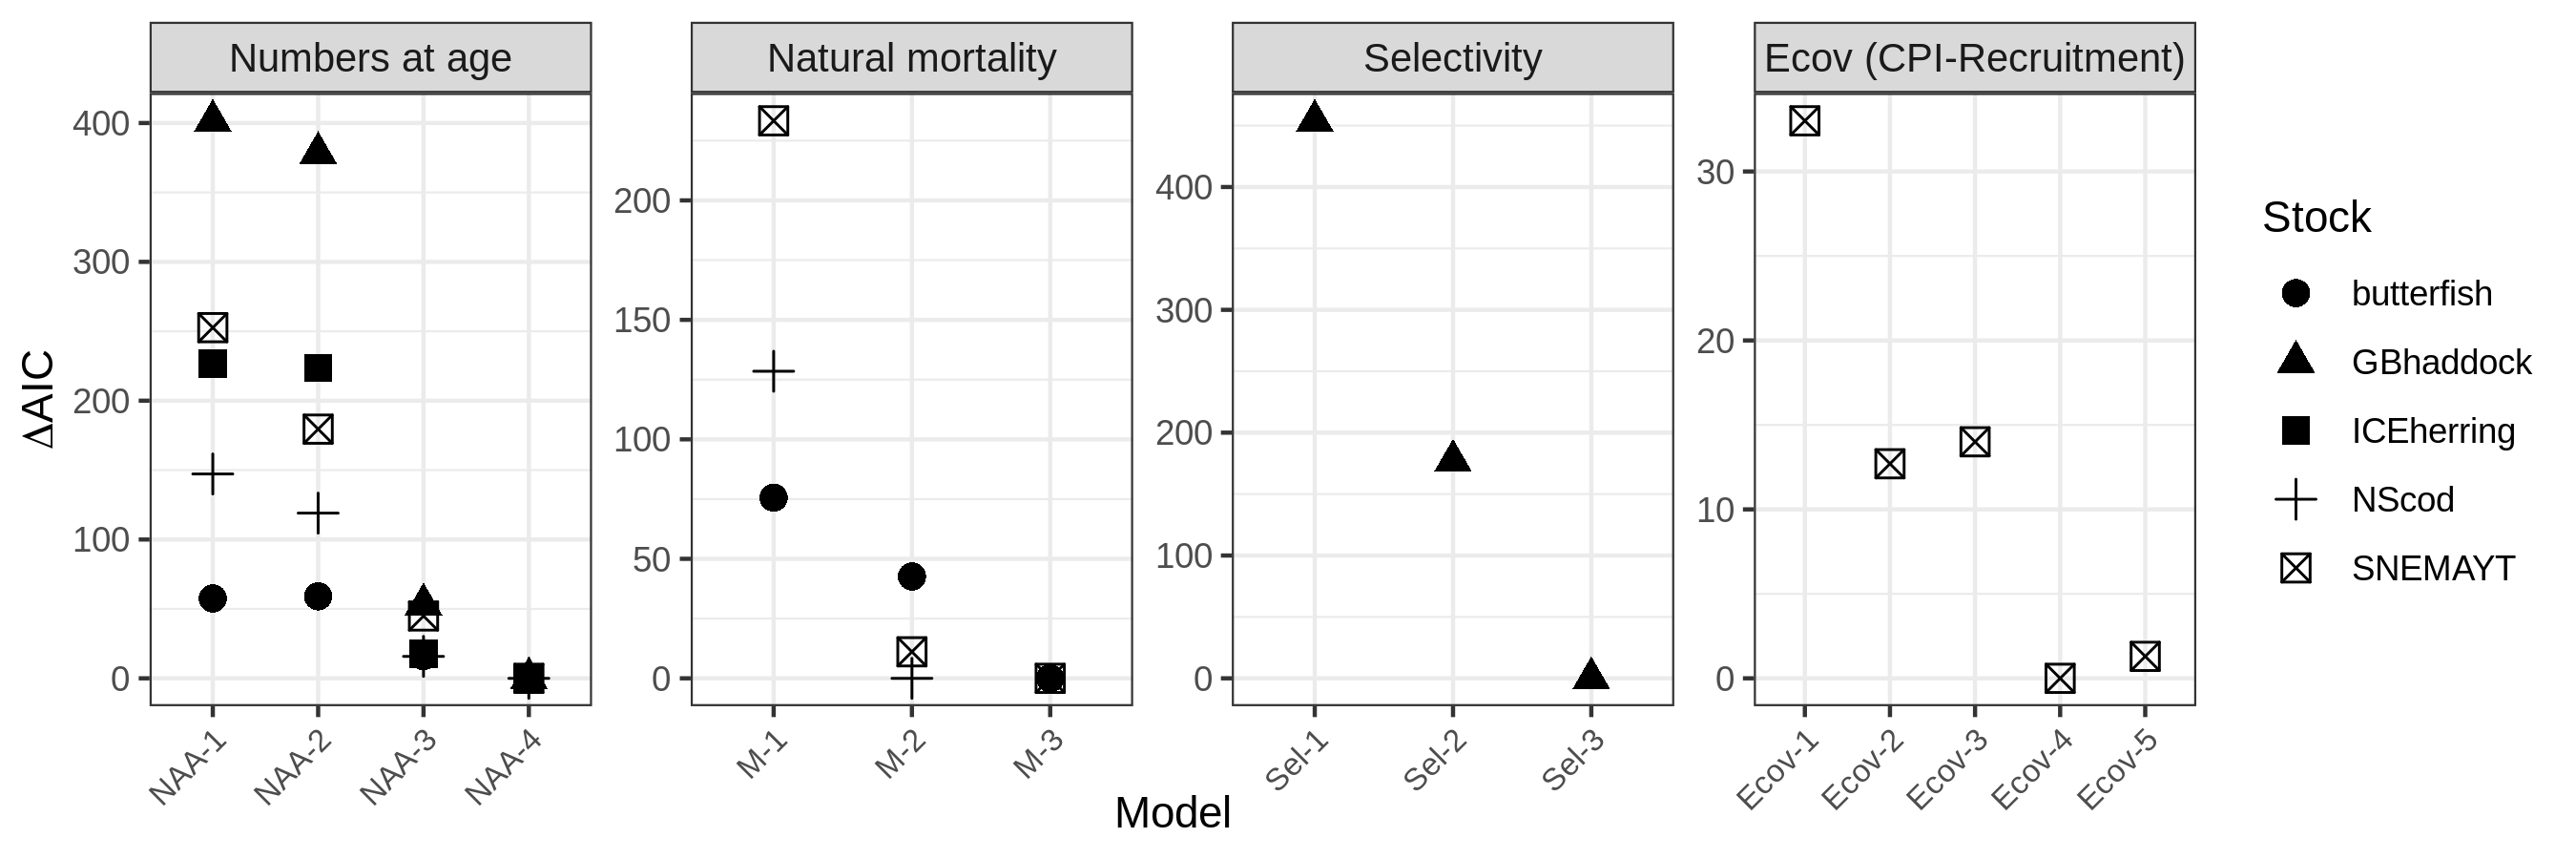
\includegraphics[width=8in]{/home/bstock/Documents/ms/wham-sim/plots/v2/daic} 

}

\caption{AIC differences by model and stock when fit to original datasets. Random effects were only used for one process at a time (numbers at age, natural mortality, selectivity, and recruitment linked to the Cold Pool Index, CPI). Stock abbreviations: SNEMA yellowtail flounder (SNEMAYT), North Sea cod (NScod), Icelandic herring (ICEherring), and Georges Bank haddock (GBhaddock).}\label{fig:daic}
\end{figure}
\end{landscape}

\pagebreak

\begin{figure}

{\centering 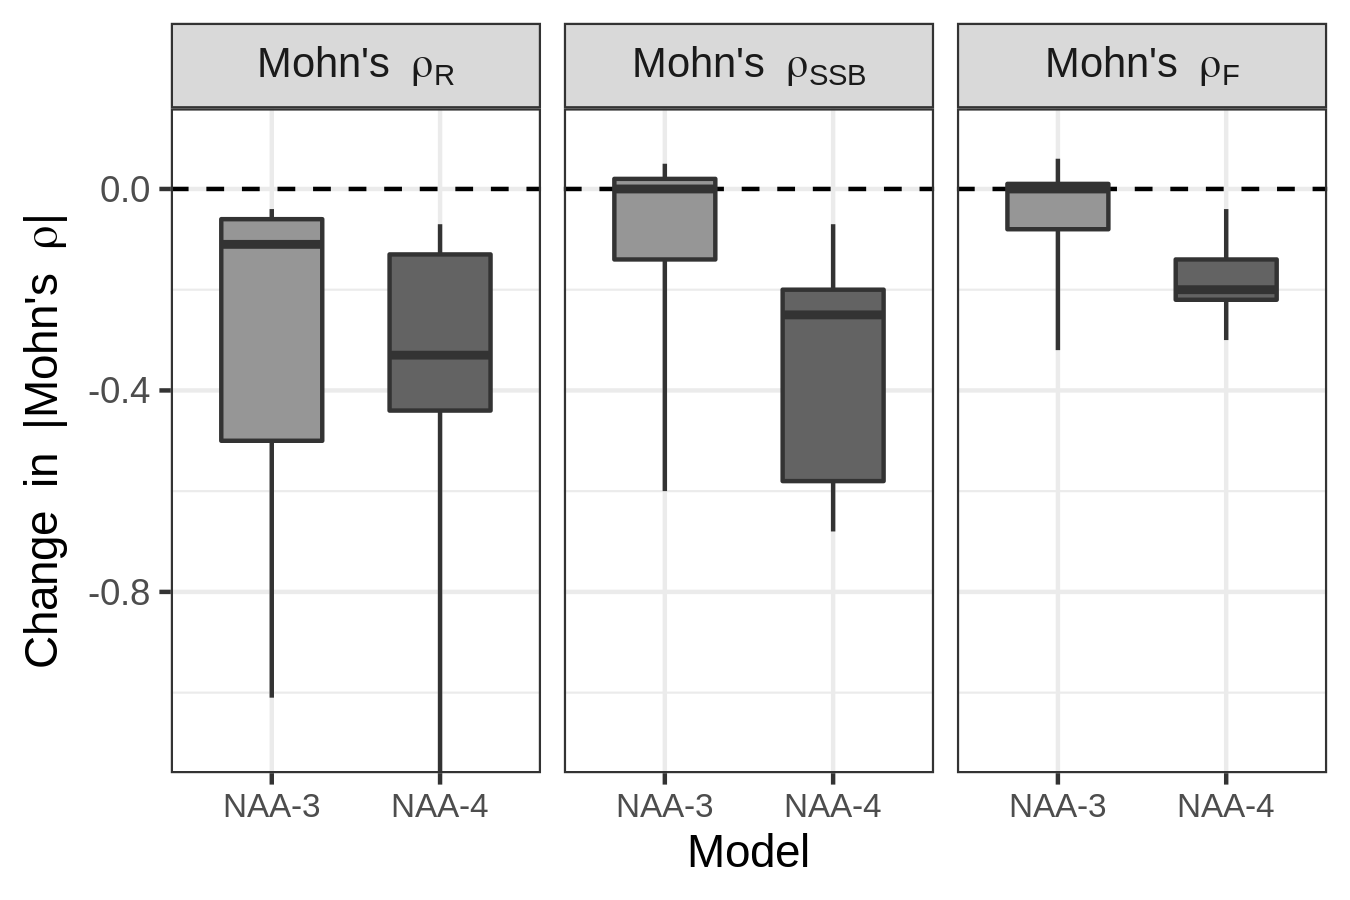
\includegraphics[width=4.5in]{/home/bstock/Documents/ms/wham-sim/plots/v2/mohns_rho_reduction_boxplot} 

}

\caption{Change in Mohn's $\rho$ relative to the statistical catch at age model (Base) for full state-space models (numbers at all ages are random effects, NAA-3 and NAA-4). Changes in Mohn's $\rho$ are shown for all five stocks (whisker and box ends and median line in boxplots). Reduction in Mohn's $\rho_R$ for SNEMA yellowtail flounder NAA-4 is off chart.}\label{fig:mohns}
\end{figure}

\pagebreak

\begin{figure}

{\centering 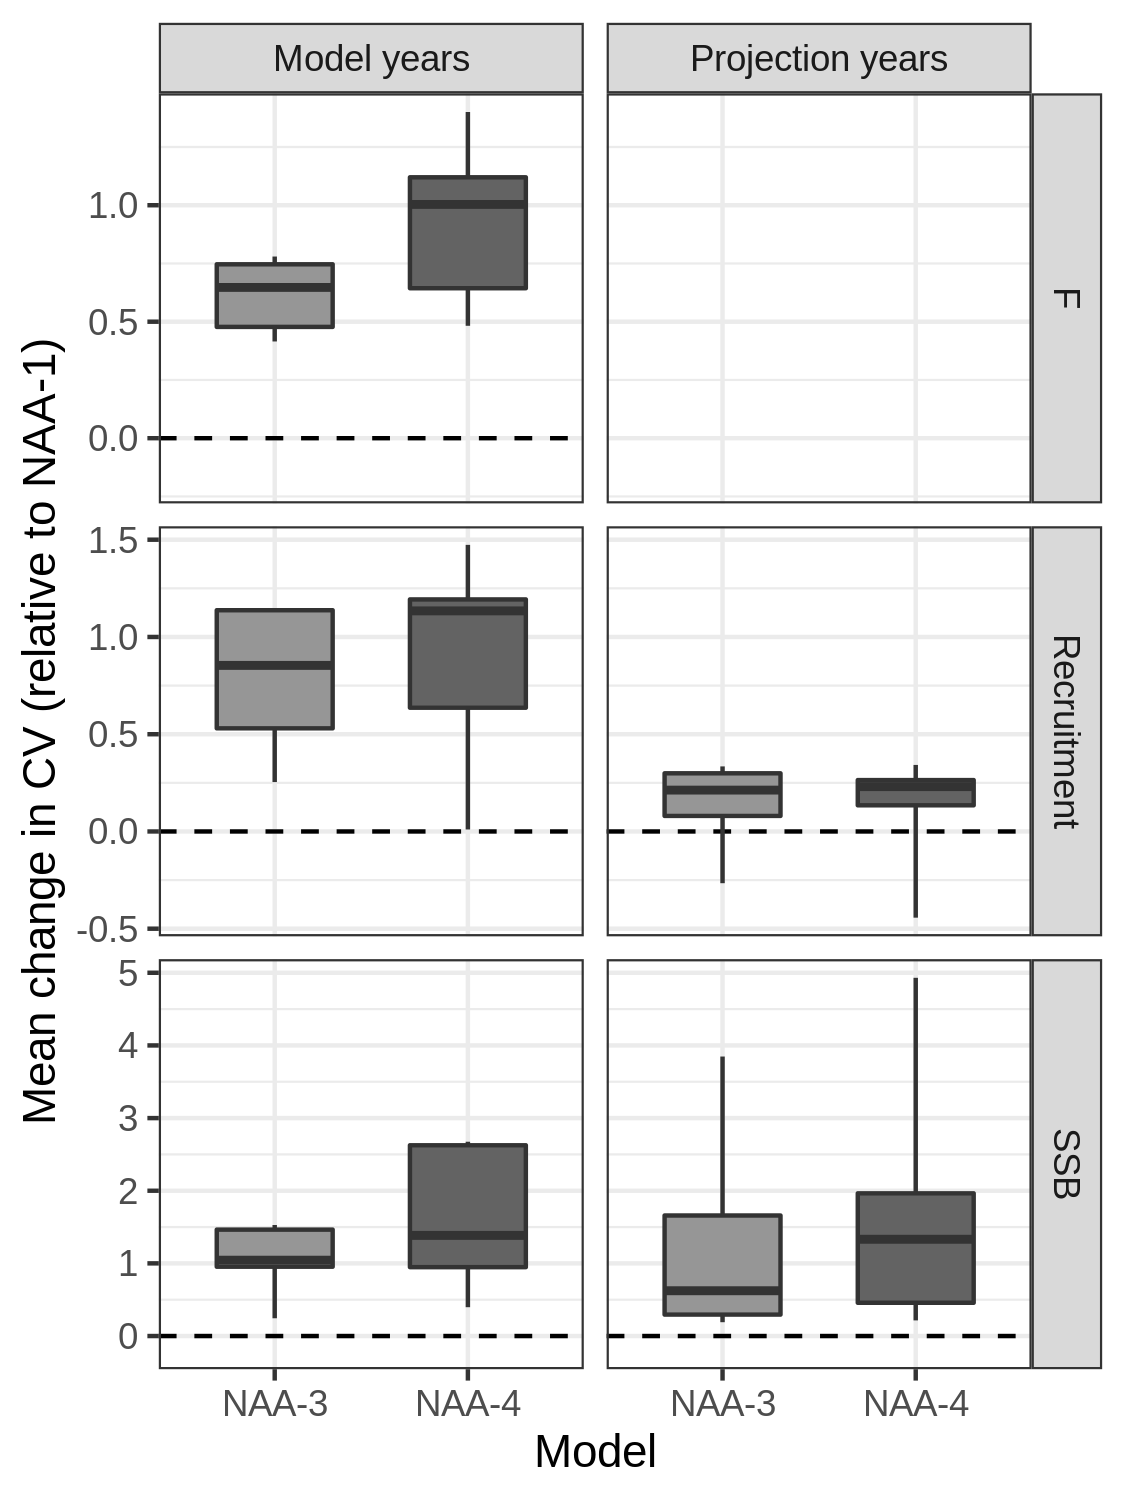
\includegraphics[width=3.75in]{/home/bstock/Documents/ms/wham-sim/plots/v2/rel_cv_naa_boxplot} 

}

\caption{Mean change in coefficient of variation (CV) for key quantities in model and projection years for full state-space models (numbers at all ages are random effects, NAA-3 and NAA-4) relative to NAA-1. Boxplots show mean change in CV across years for all five stocks (whisker and box ends, median line). $F$ was fixed at 0 in projection years.}\label{fig:cv}
\end{figure}

\pagebreak

\begin{figure}

{\centering 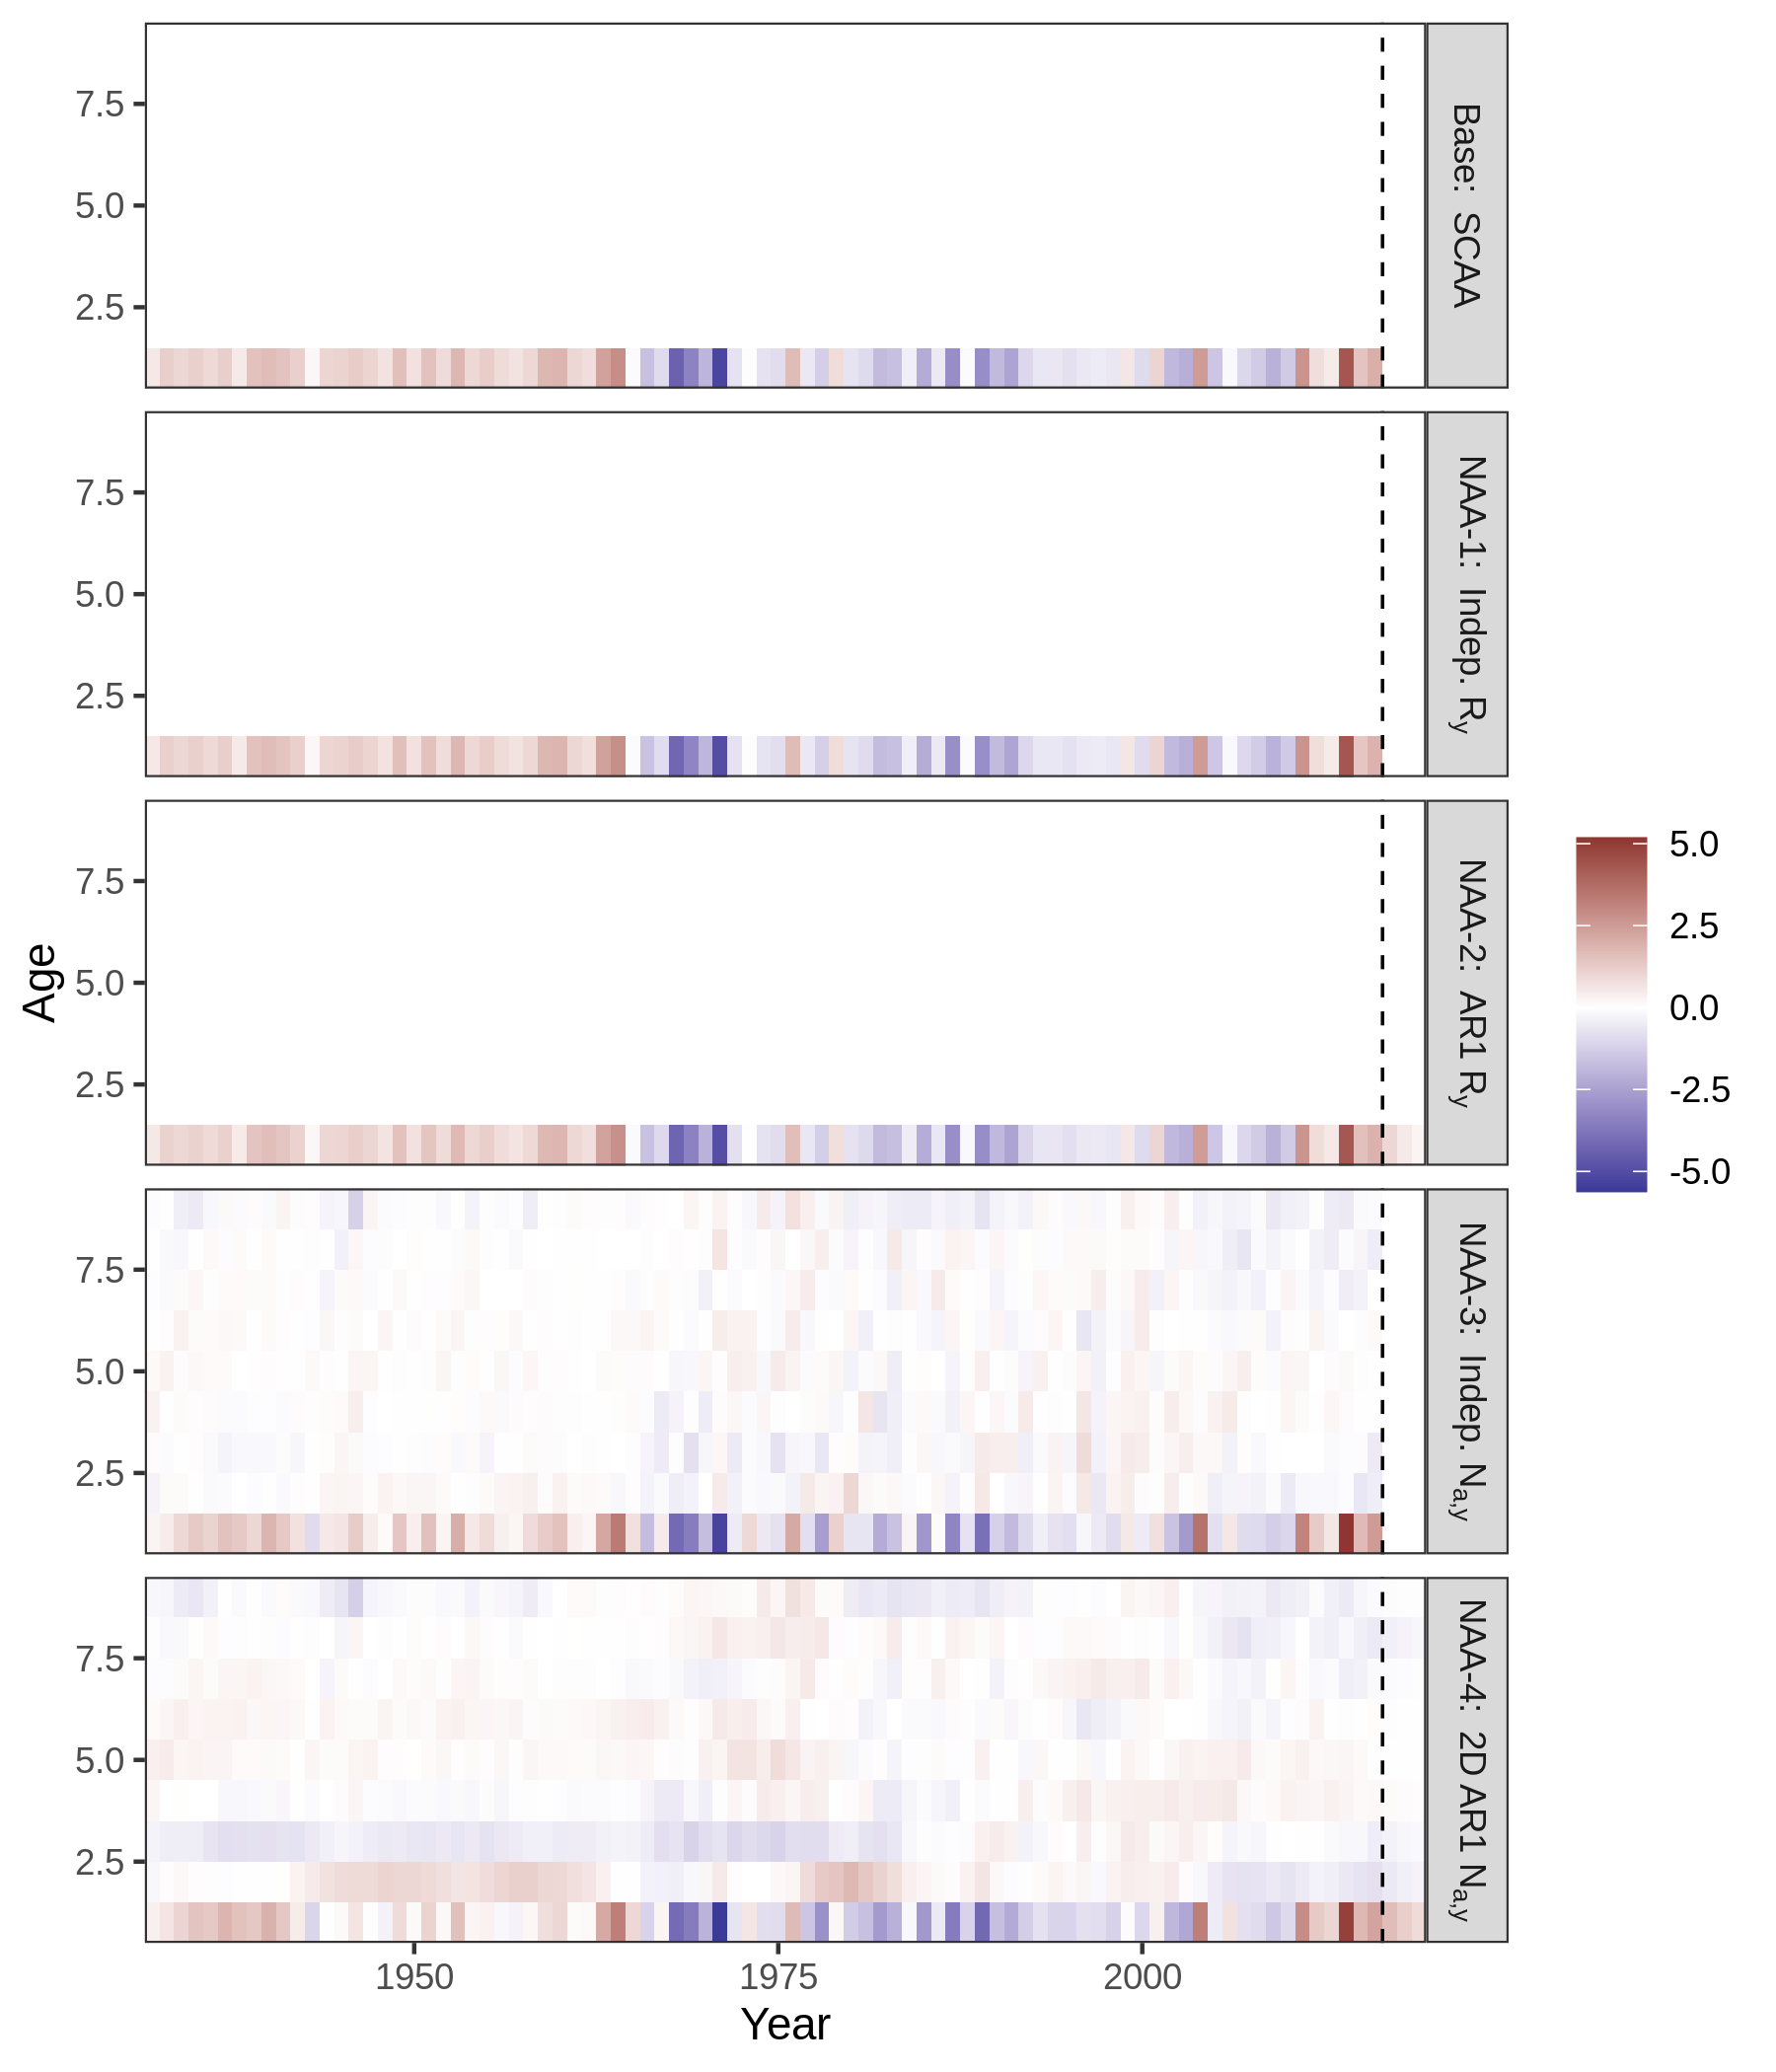
\includegraphics[width=6.5in]{/home/bstock/Documents/ms/wham-sim/plots/v2/NAAdevs_GBhaddock} 

}

\caption{Abundance-at-age deviations estimated for Georges Bank haddock using alternative models of numbers-at-age (NAA) random effects. Base = a traditional statistical catch-at-age (SCAA) model. NAA-1 = only recruitment deviations are independent random effects (most similar to Base). NAA-2 = as NAA-1, but with autocorrelated recruitment deviations, AR(1). NAA-3 = all NAA deviations are independent random effects. NAA-4 = as NAA-3, but deviations are correlated by age ($\rho_{age} = -0.12$, 95\% CI: -0.32-0.08) and year ($\rho_{year} = 0.73$, 95\% CI: 0.58-0.87). The vertical dashed line indicates the terminal year in the assessment.}\label{fig:devs-GBhaddock-naa}
\end{figure}

\pagebreak

\begin{figure}

{\centering 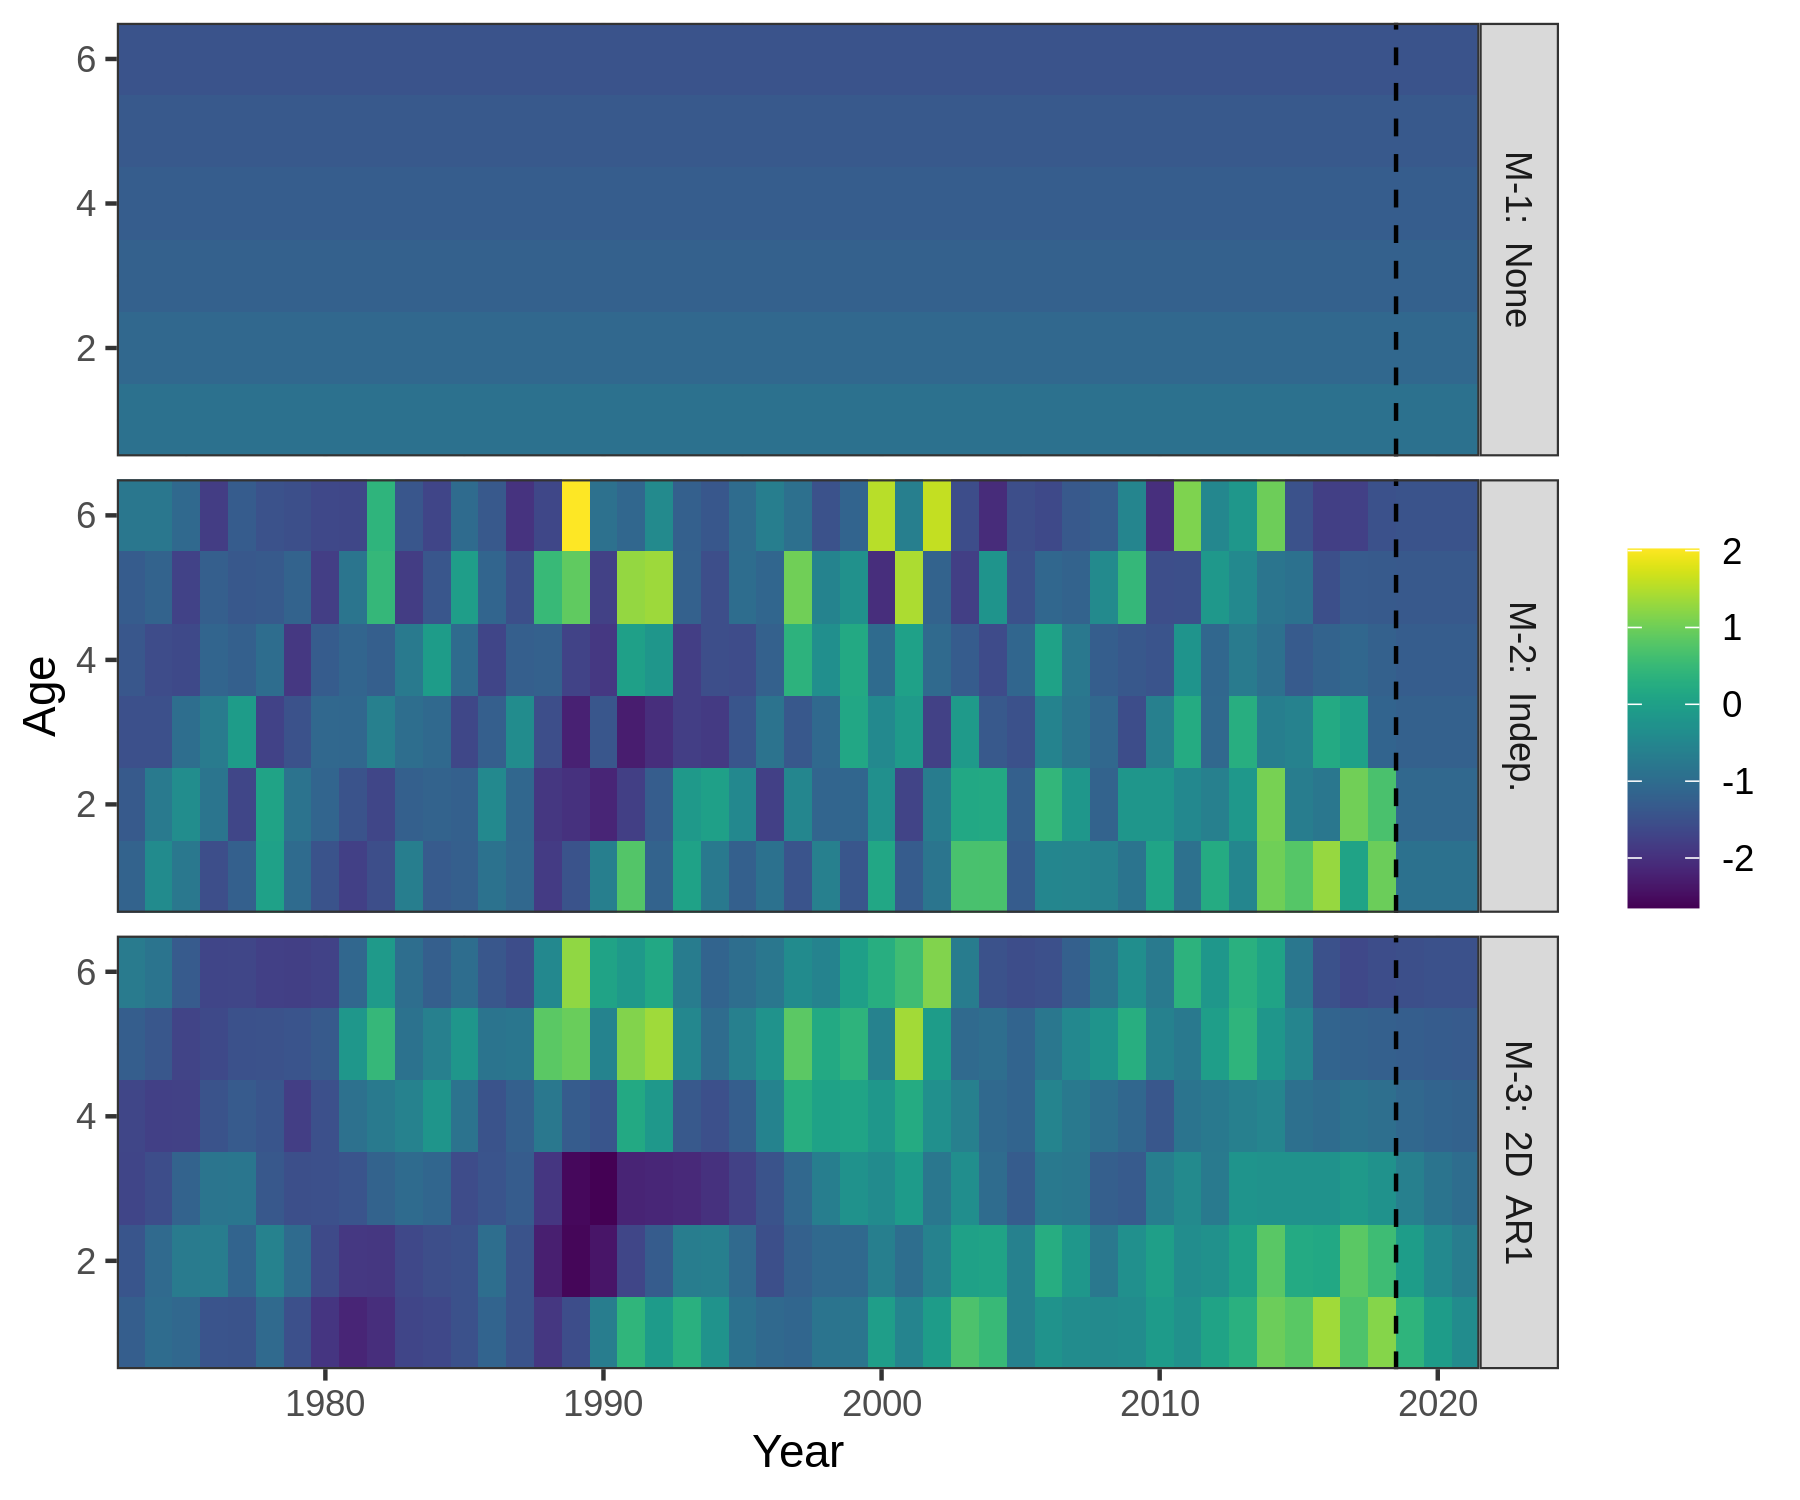
\includegraphics[width=6in]{/home/bstock/Documents/ms/wham-sim/plots/v2/logM_SNEMAYT} 

}

\caption{Natural mortality, log(\textit{M}), estimated for Southern New England-Mid Atlantic yellowtail flounder using three random effects models. M-1 = no random effects on \textit{M}. M-2 = independent \textit{M} deviations. M-3 = \textit{M} deviations are correlated by age ($\varphi_{age} = 0.40$, 95\% CI: 0.09-0.70) and year ($\varphi_{year} = 0.63$, 95\% CI: 0.31-0.94). The vertical dashed line indicates the terminal year in the assessment.}\label{fig:devs-snemayt-m}
\end{figure}

\pagebreak

\begin{figure}

{\centering 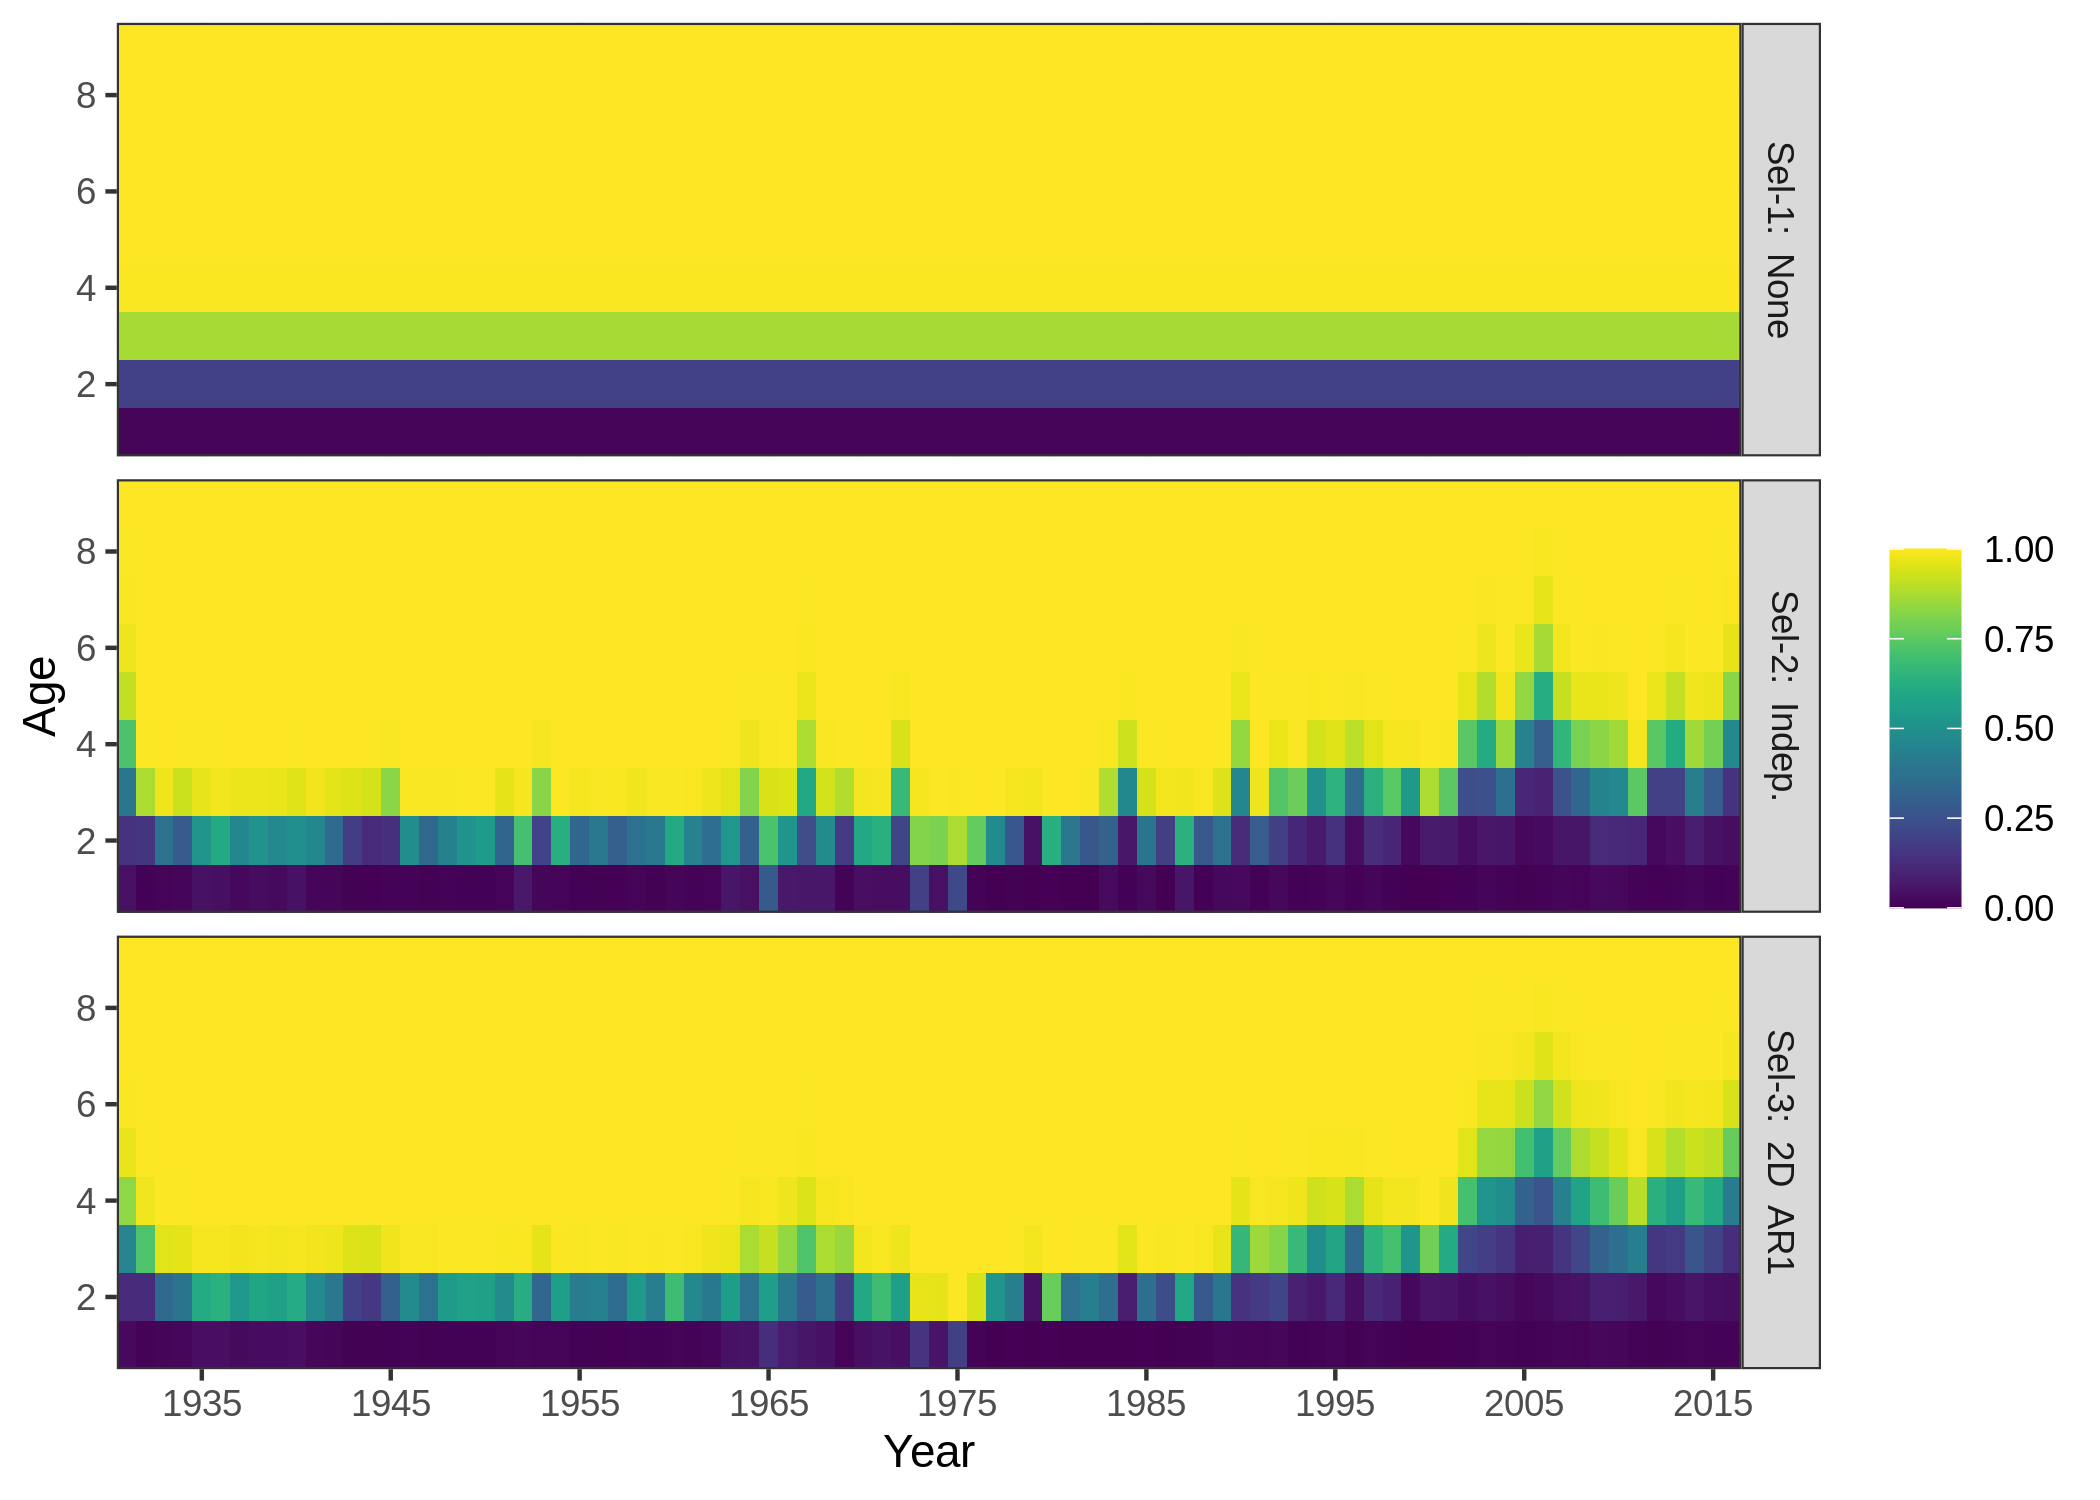
\includegraphics[width=6.5in]{/home/bstock/Documents/ms/wham-sim/plots/v2/Sel_GBhaddock} 

}

\caption{Selectivity estimated for Georges Bank haddock using three random effects models. Sel-1 = no random effects (constant logistic selectivity). Sel-2 = independent selectivity deviations. Sel-3 = selectivity deviations are correlated by parameter ($\phi_{par} = 0.60$, 95\% CI: 0.30-0.80) and year ($\phi_{year} = 0.87$, 95\% CI: 0.74-0.94).}\label{fig:devs-GBhaddock-sel}
\end{figure}

\pagebreak

\begin{figure}

{\centering 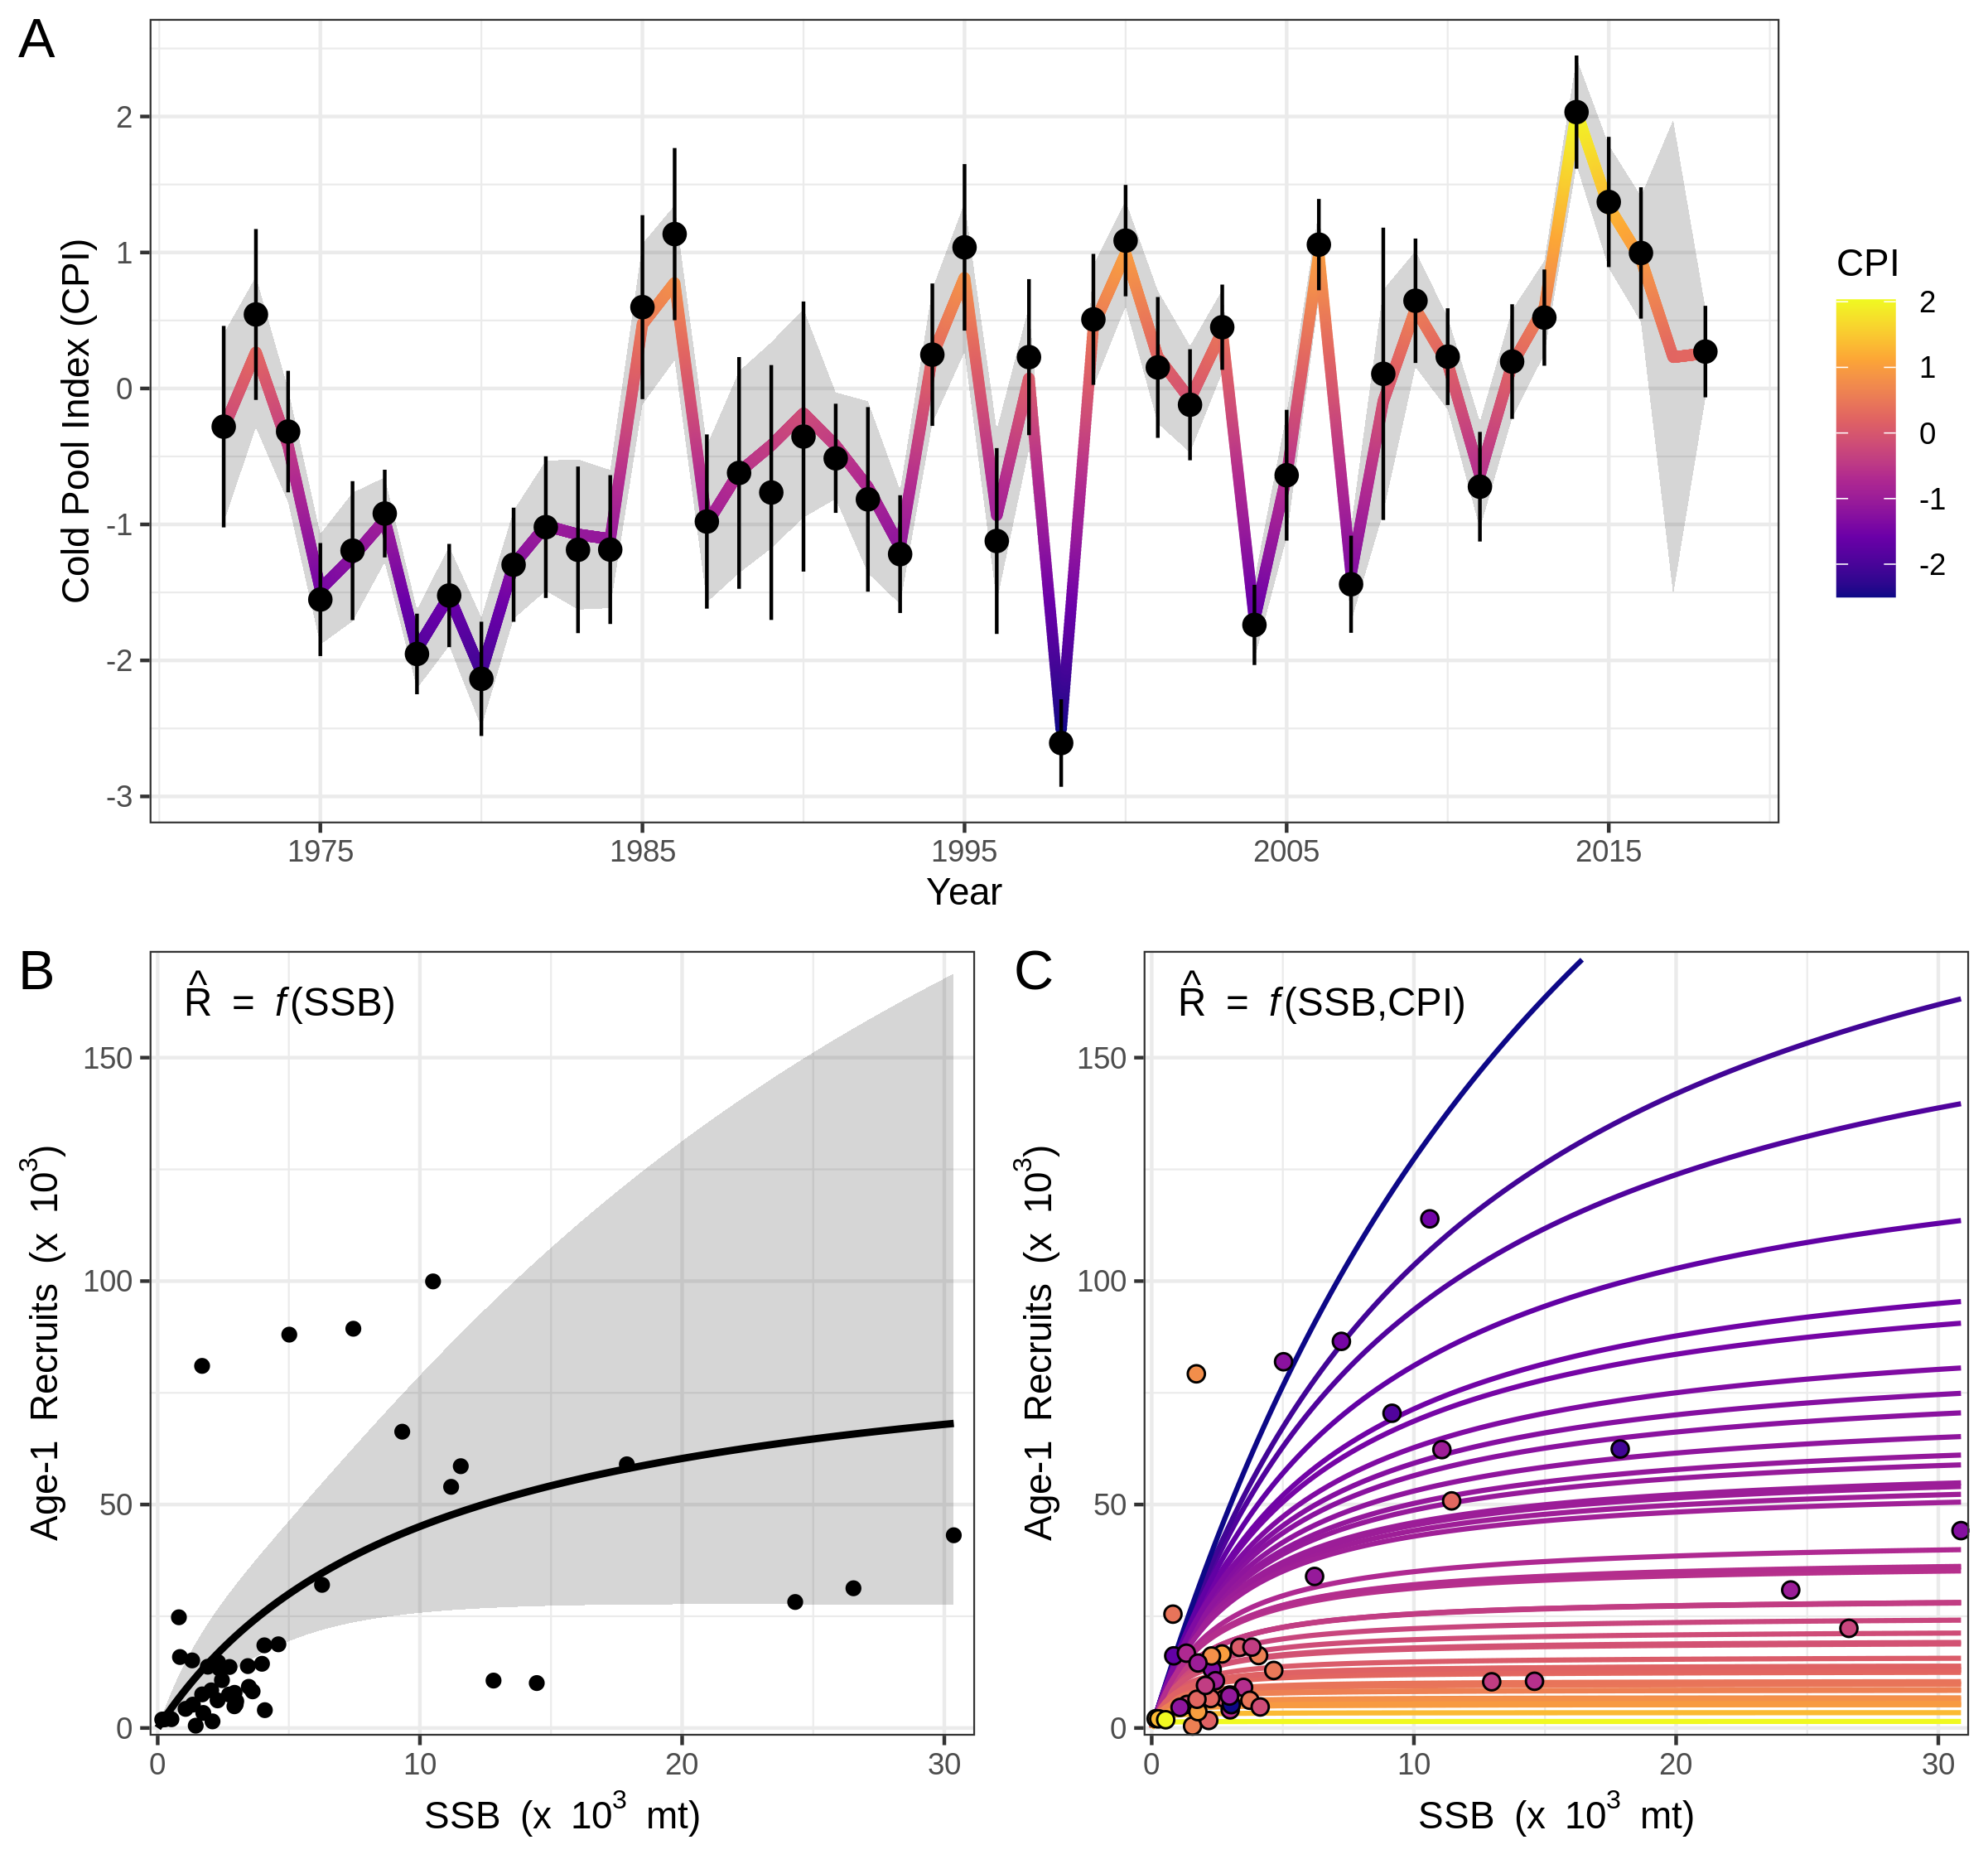
\includegraphics[width=6.5in]{/home/bstock/Documents/ms/wham-sim/plots/v2/CPI_Recruit_SNEMAYT} 

}

\caption{Beverton-Holt stock-recruit relationships fit for Southern New England-Mid Atlantic yellowtail flounder, with and without effects of the Cold Pool Index (CPI). A) CPI estimated from the model with lowest AIC (Ecov-4, AR(1)-linear). Points are observations with 95\% CI, and the line with shading is the model-estimated CPI with 95\% CI. Note the increased uncertainty surrounding the CPI estimate in 2017 (no observation). B) Estimates of spawning stock biomass (SSB), recruitment, and the stock-recruit function from the model without a CPI effect, Ecov-1. C) Estimates of SSB and recruitment from Ecov-4, with an effect of the CPI on $\beta$. Lines depict the expected stock-recruit relationship in each year $y$, given the CPI in year $y-1$ (color).}\label{fig:devs-SNEMAYT-ecov}
\end{figure}

\pagebreak

\begin{figure}

{\centering 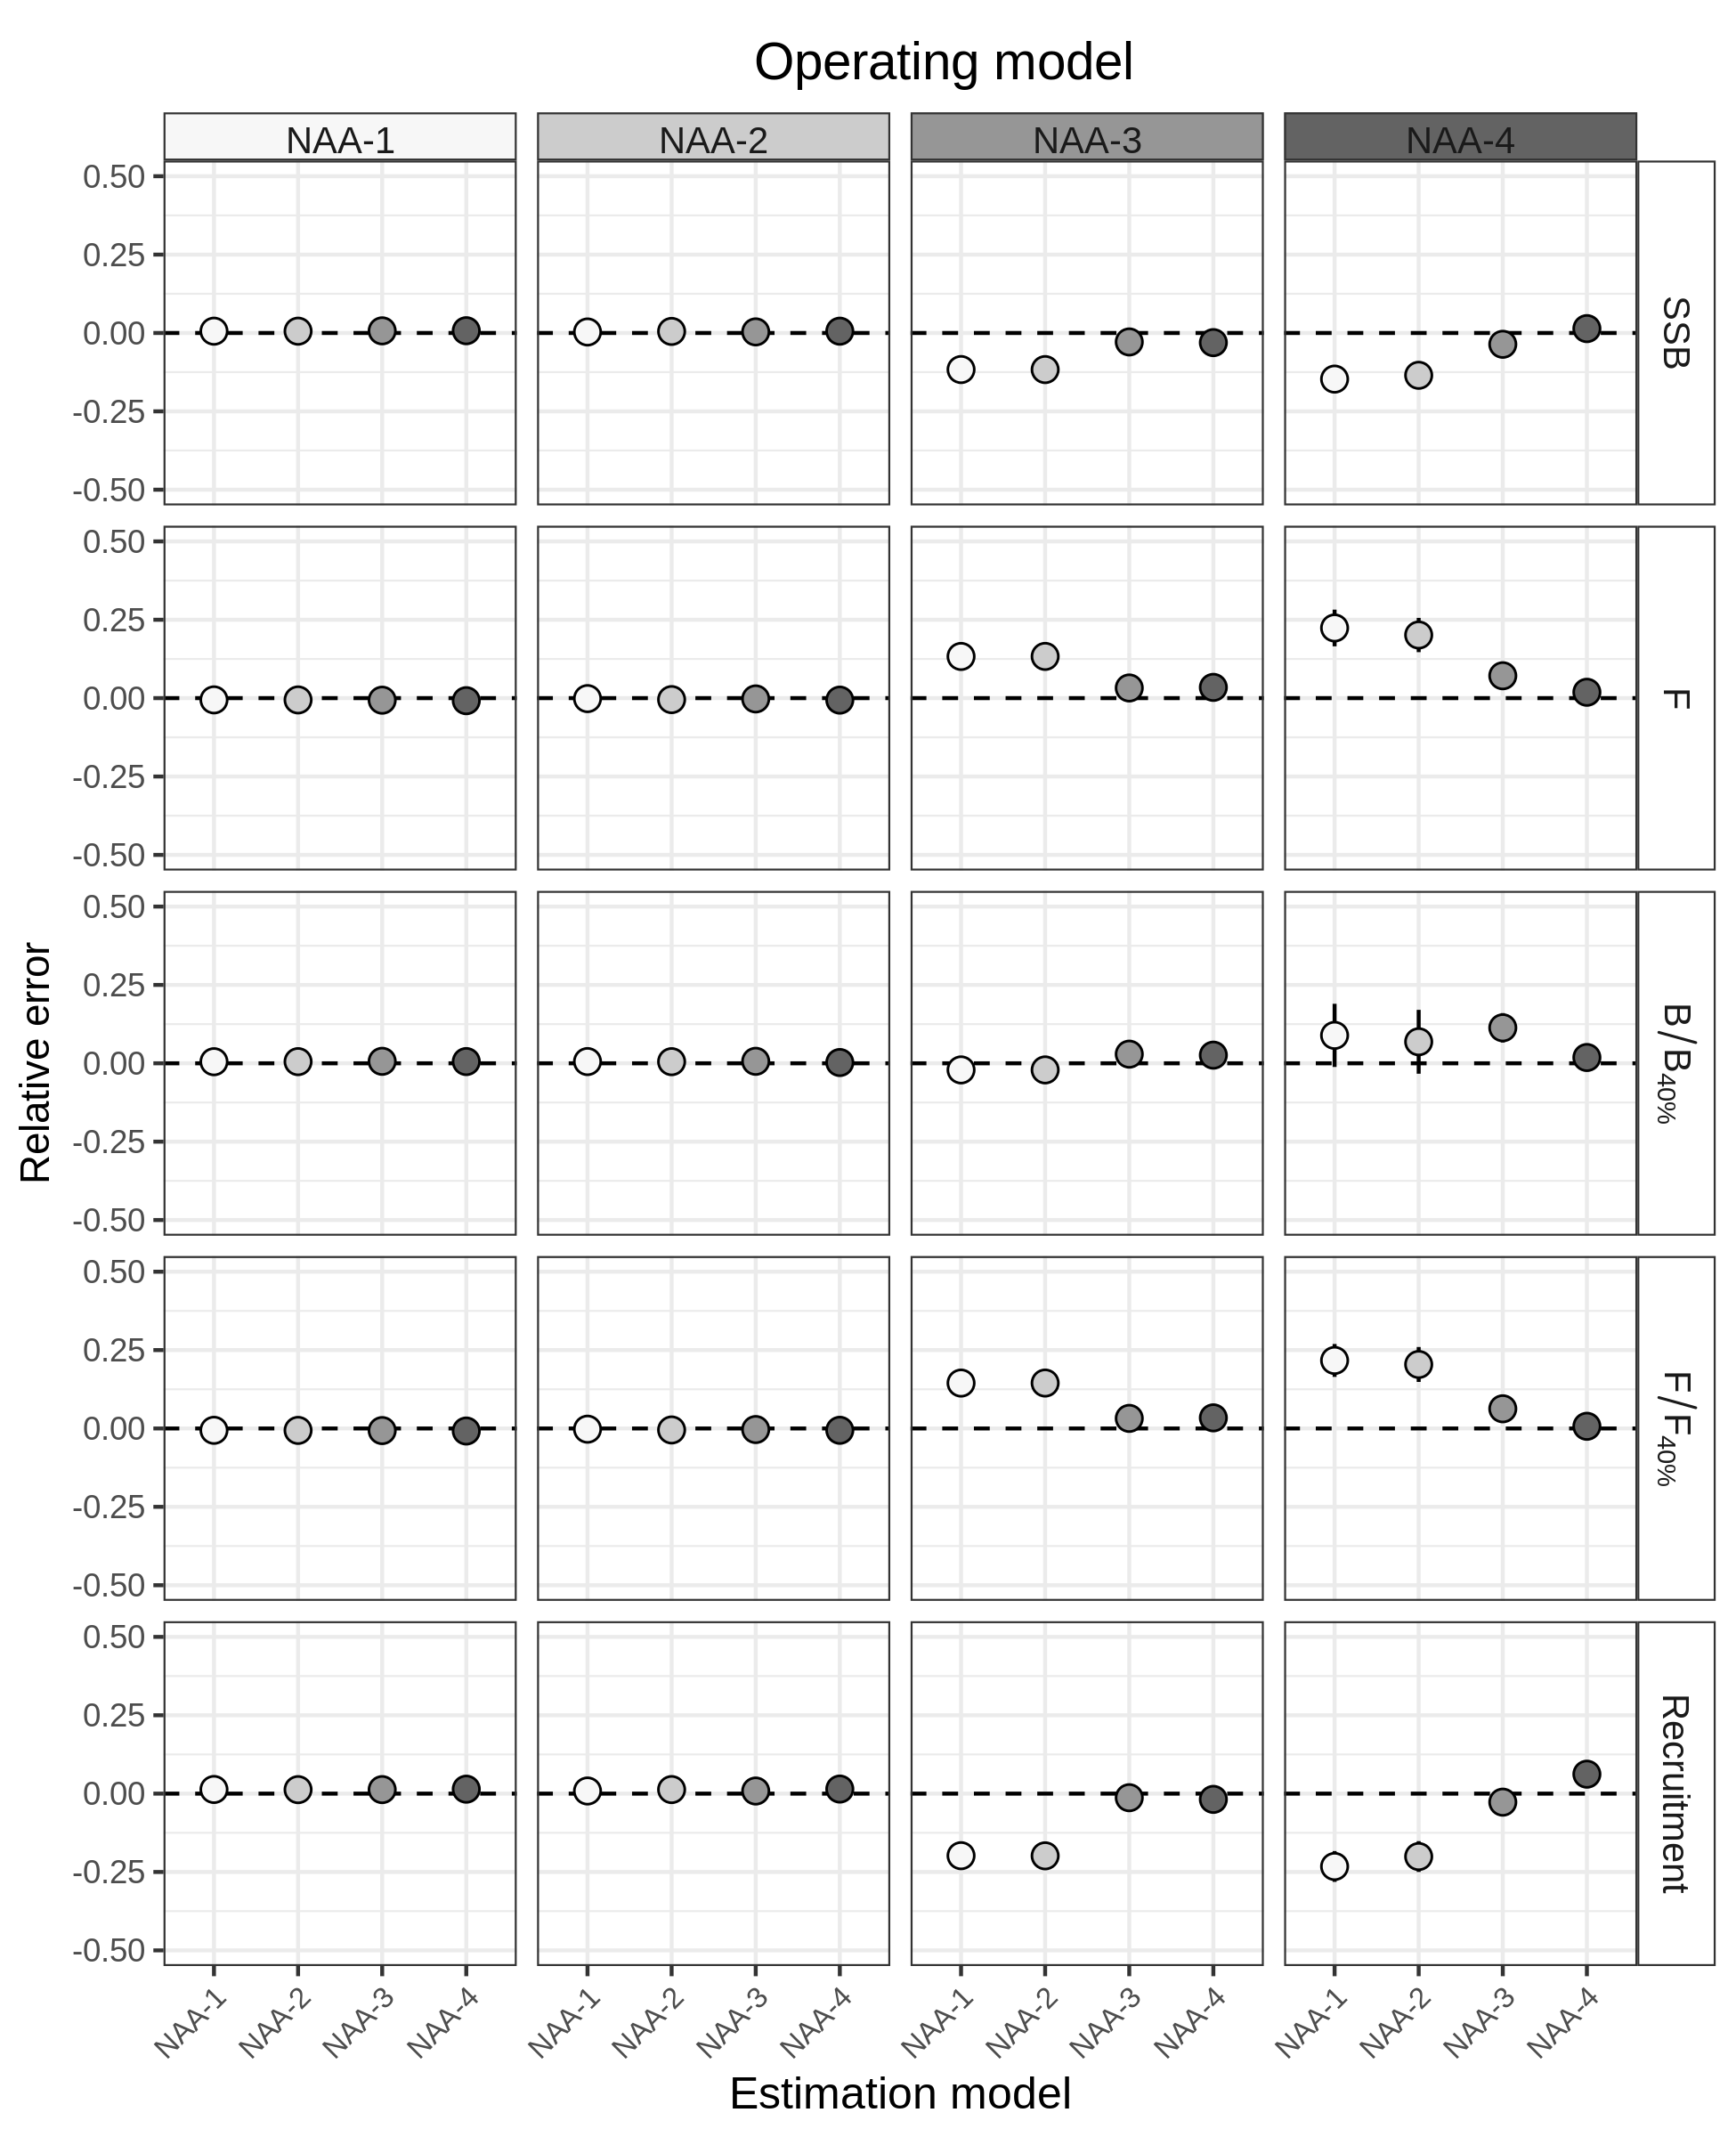
\includegraphics[width=6.5in]{/home/bstock/Documents/ms/wham-sim/plots/v2/GBhaddock_NAA_medianCI_OEPE} 

}

\caption{Relative error of key quantities estimated for Georges Bank haddock using four models of numbers-at-age (NAA) random effects. NAA-1 = only recruitment deviations are random effects (most similar to Base, a traditional statistical catch-at-age model), and deviations are independent. NAA-2 = as NAA-1, but with autocorrelated recruitment deviations. NAA-3 = all NAA deviations are independent random effects. NAA-4 = as NAA-3, but deviations are correlated by age and year. Points without lines indicate that 95\% CI are smaller than the points.}\label{fig:rel-error-GBhaddock-naa}
\end{figure}

\pagebreak

\begin{figure}

{\centering 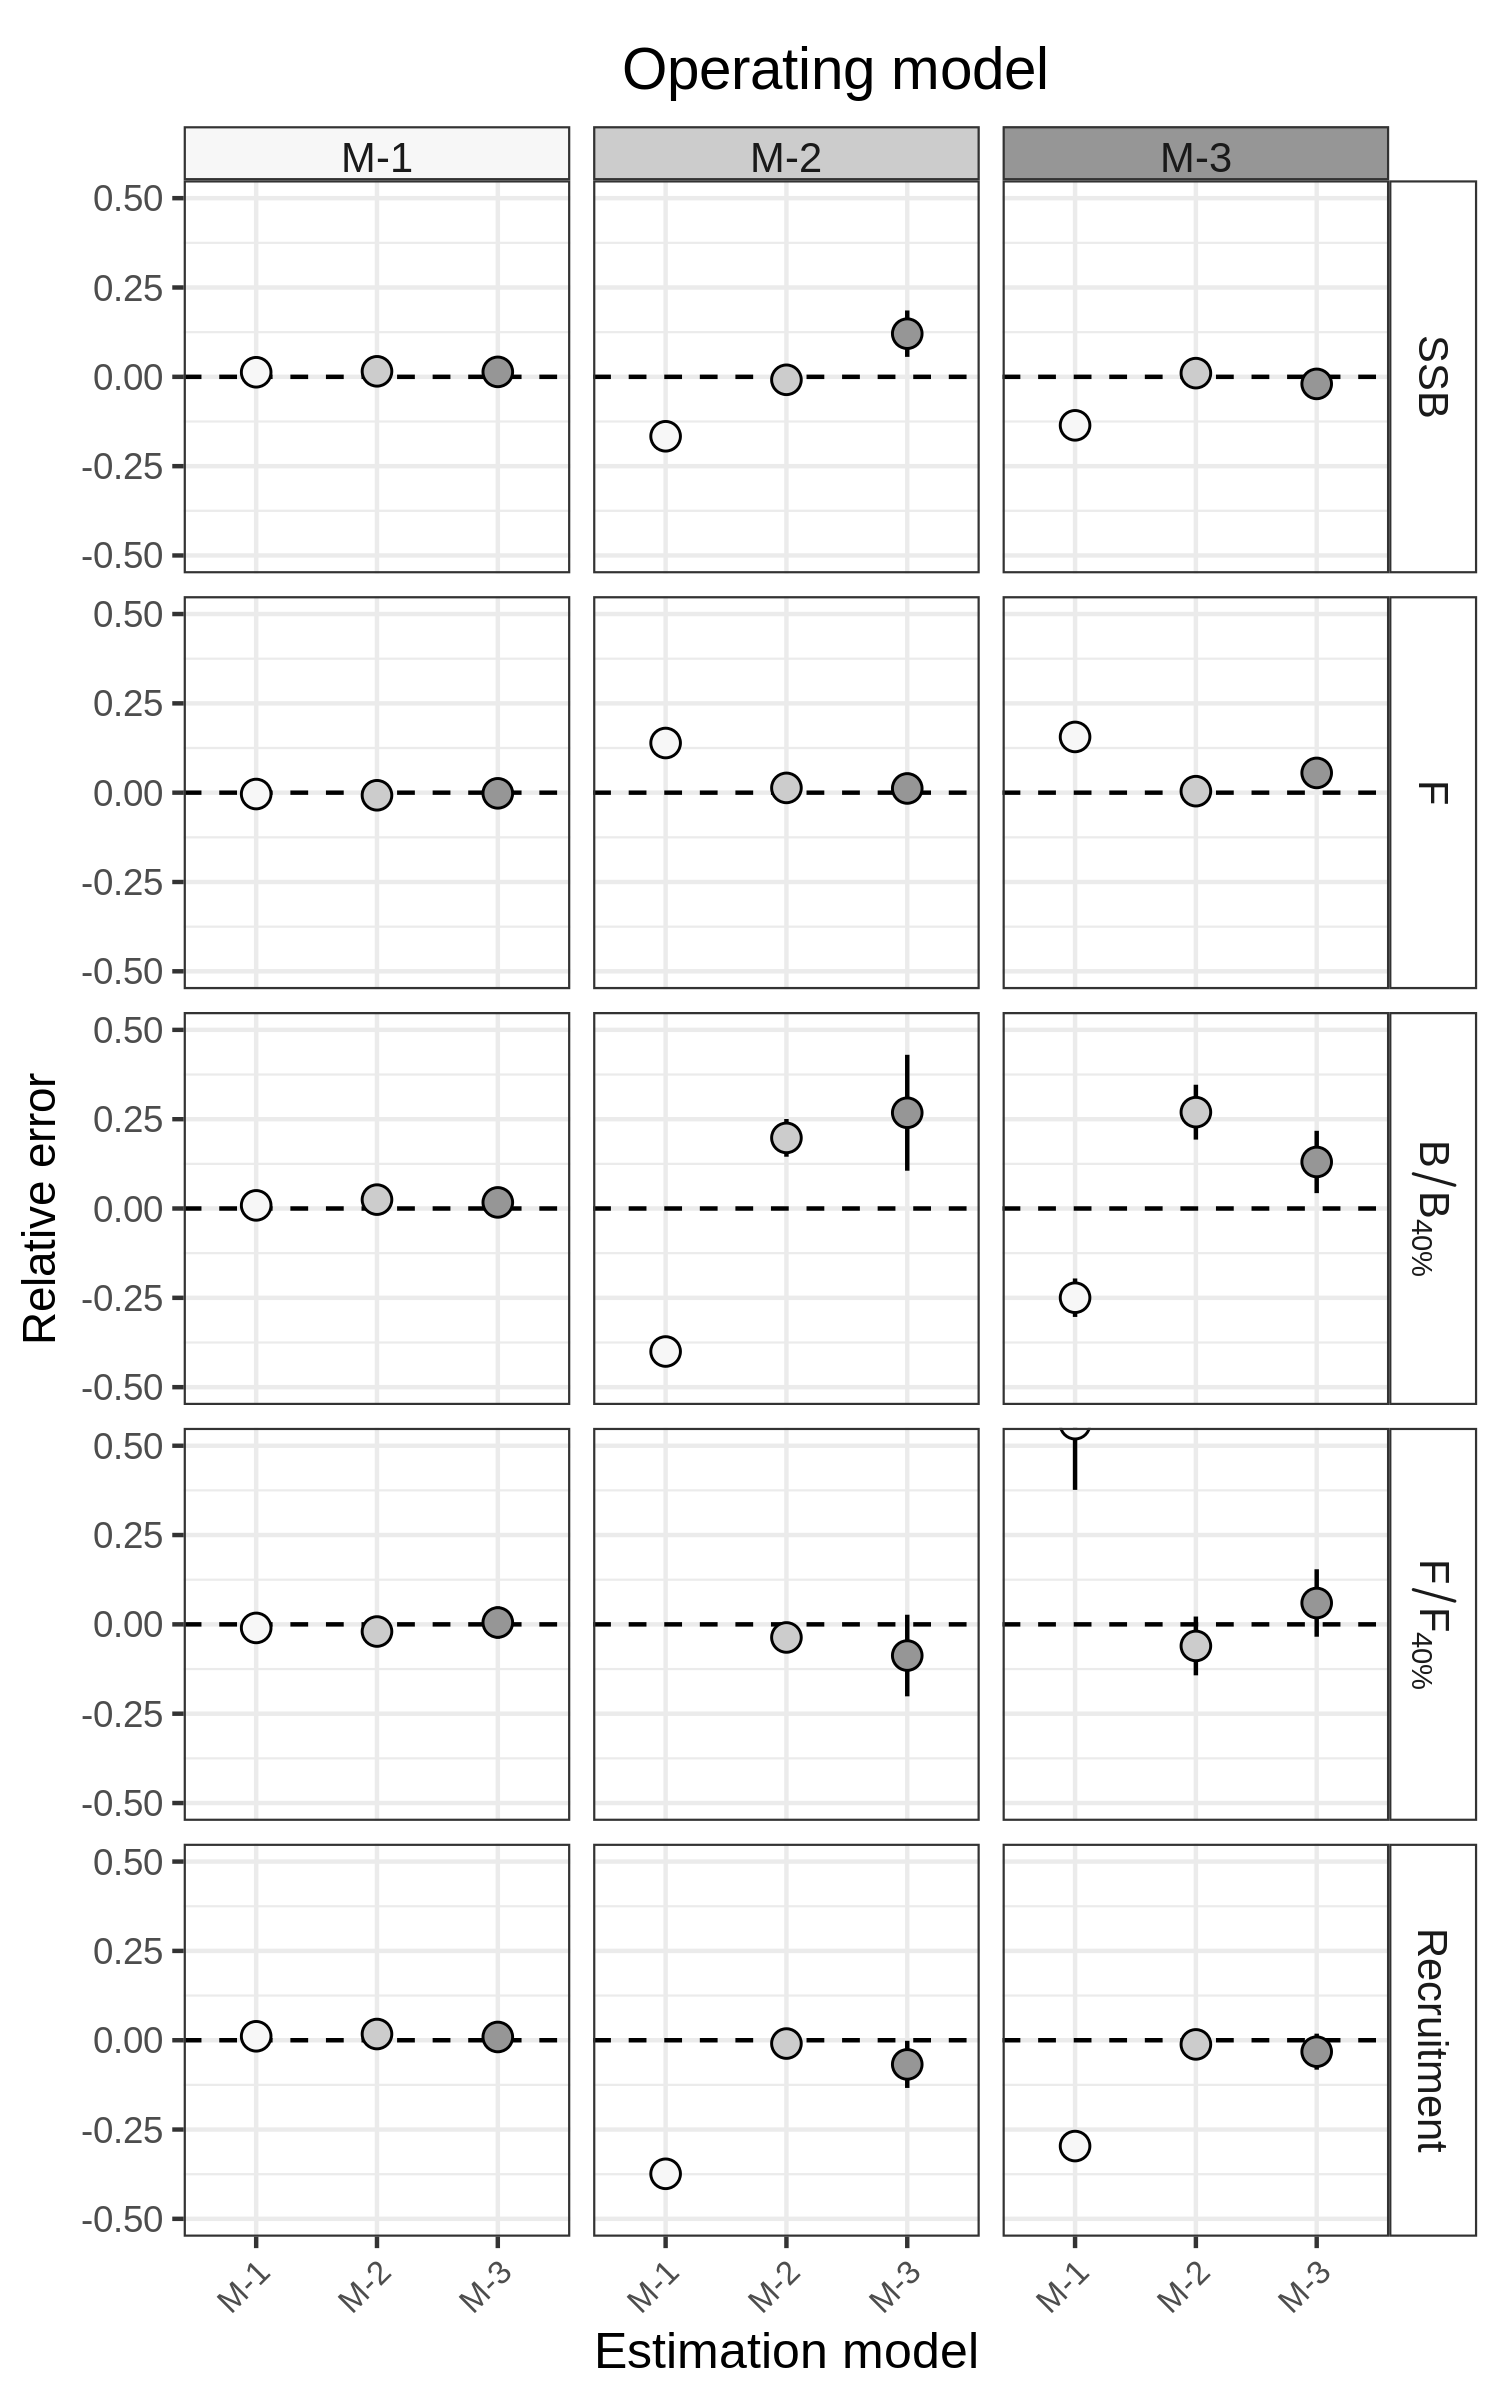
\includegraphics[width=5in]{/home/bstock/Documents/ms/wham-sim/plots/v2/SNEMAYT_M_medianCI_OEPE} 

}

\caption{Relative error of key quantities estimated for Southern New England-Mid Atlantic yellowtail flounder using three models of natural mortality (\textit{M}) random effects. M-1 = no random effects on \textit{M}. M-2 = independent \textit{M} deviations. M-3 = \textit{M} deviations are correlated by age and year. Points without lines indicate that 95\% CI are smaller than the points.}\label{fig:rel-error-snemayt-m}
\end{figure}

\pagebreak

\begin{figure}

{\centering 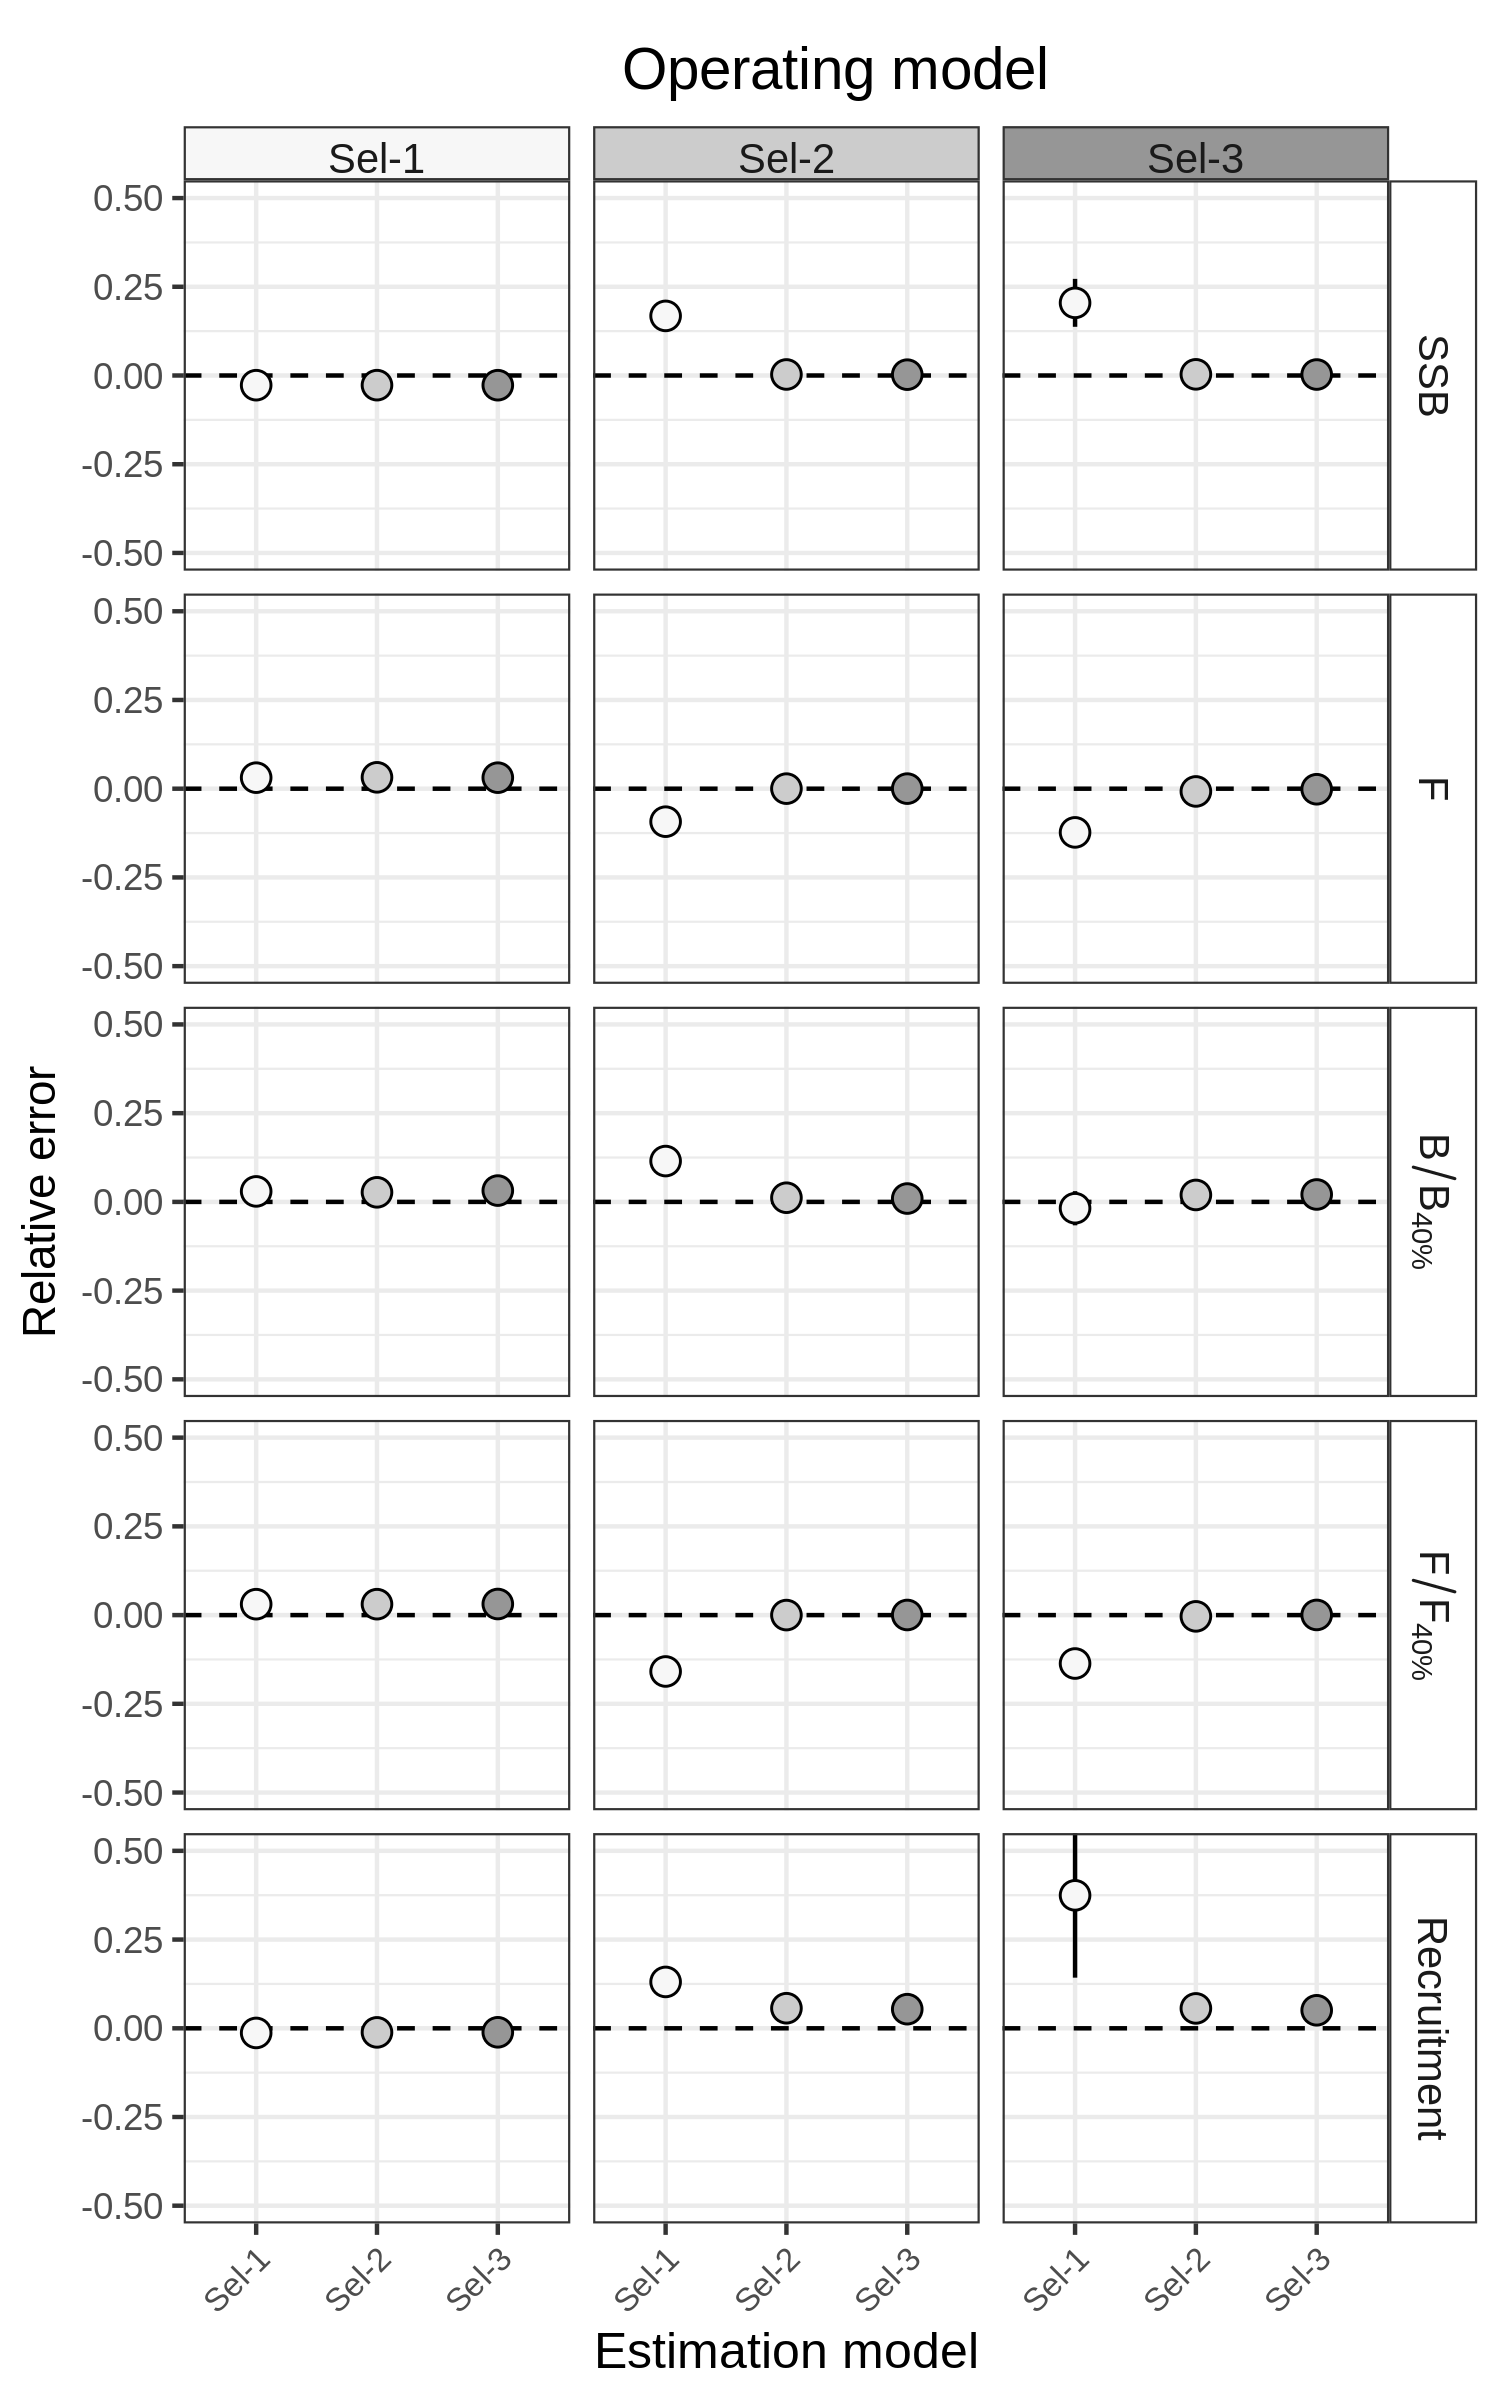
\includegraphics[width=5in]{/home/bstock/Documents/ms/wham-sim/plots/v2/GBhaddock_sel_medianCI_OEPE} 

}

\caption{Relative error of key quantities estimated for Georges Bank haddock using three models of selectivity random effects. Sel-1 = no random effects (constant logistic selectivity). Sel-2 = independent selectivity deviations. Sel-3 = selectivity deviations are correlated by parameter and year. Points without lines indicate that 95\% CI are smaller than the points.}\label{fig:rel-error-GBhaddock-sel}
\end{figure}

\pagebreak

\begin{figure}

{\centering 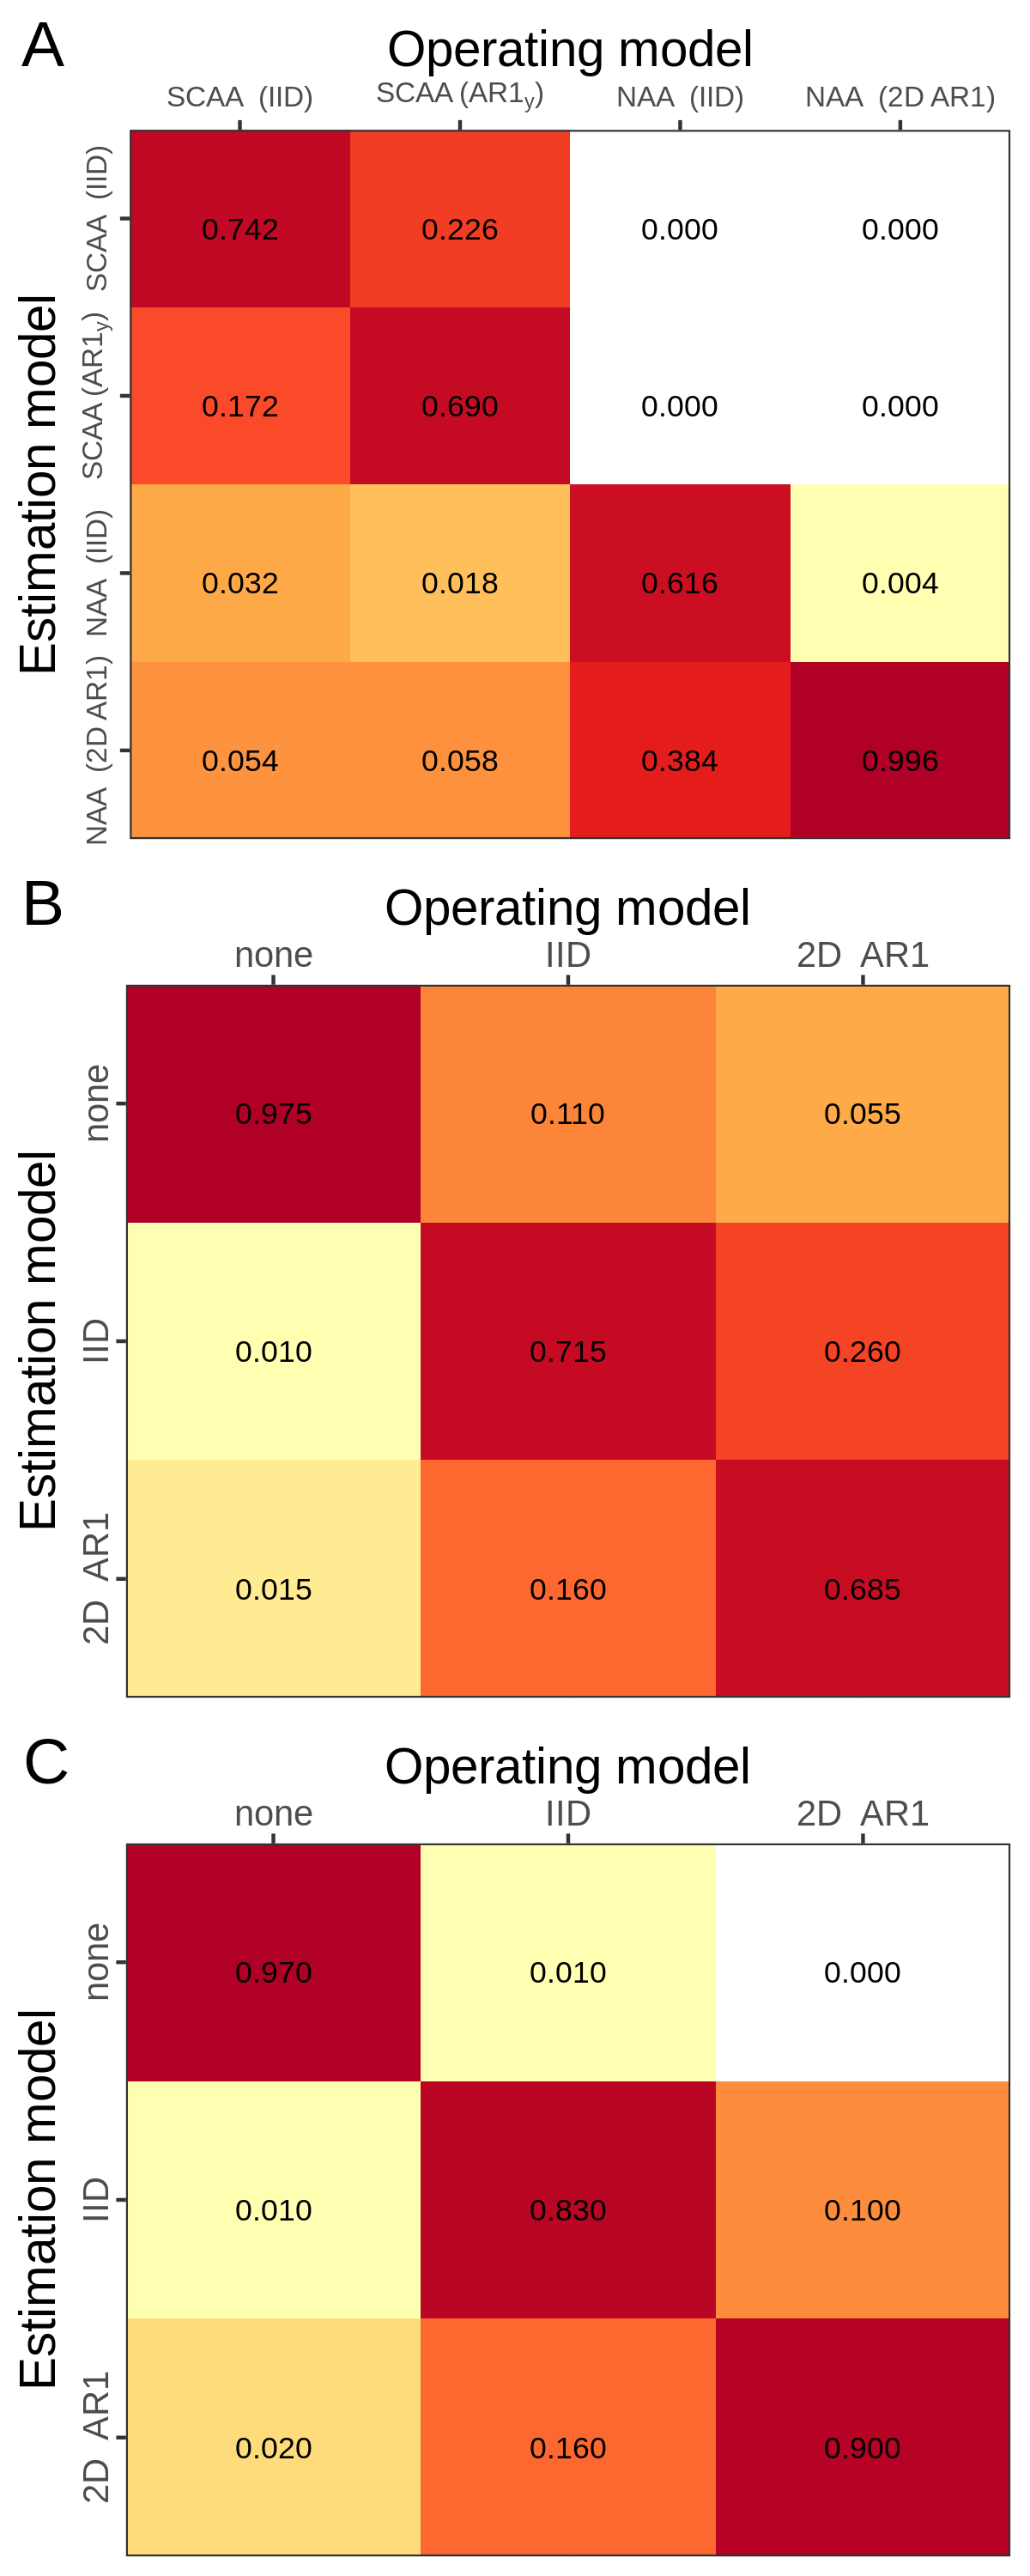
\includegraphics[width=3.5in]{/home/bstock/Documents/ms/wham-sim/plots/v1/into_paper/aic_cross_multipanel} 

}

\caption{Proportion of simulations in which each model had the lowest AIC. A) Numbers-at-age (NAA), aggregated across all five stocks. B) Natural mortality (\textit{M}), aggregated over two stocks (SNEMAYT and butterfish). C) Selectivity (GBhaddock). Not all estimation models converged for each simulation, even when the operating model matched.}\label{fig:aic-cross}
\end{figure}

\end{document}
